% Shared preamble for the Persian B.Sc. report.
% Compile with XeLaTeX + biber. See compile.ps1.

\documentclass[a4paper,14pt,oneside,openany]{extbook}

\usepackage{iftex}
\RequireXeTeX

\usepackage[
  a4paper,
  top=2.7cm,
  bottom=2.7cm,
  right=3.0cm,
  left=2.5cm,
  headheight=22pt
]{geometry}

\usepackage{amsmath,amssymb,amsthm}
\usepackage{mathtools}
\usepackage{bm}
\usepackage{graphicx}
\usepackage{xcolor}
\usepackage{booktabs}
\usepackage{array}
\usepackage{tabularx}
\usepackage{longtable}
\usepackage{multirow}
\usepackage{makecell}
\usepackage{adjustbox}
\renewcommand{\tabularxcolumn}[1]{>{\hspace{0pt}}p{#1}}
\usepackage{caption}
\usepackage{subcaption}
\usepackage{float}
\usepackage{setspace}
\usepackage{enumitem}
\usepackage{fancyhdr}
\usepackage{titlesec}
\makeatletter
\providecommand{\ttl@finishall}{}
\makeatother
\usepackage{csquotes}
\usepackage{xurl}
\usepackage{newunicodechar}
\usepackage{hyperref}
\usepackage[
  backend=biber,
  style=numeric,
  sorting=nyt,
  maxbibnames=8,
  minbibnames=6,
  giveninits=true,
  uniquename=init,
  isbn=false,
  doi=true,
  url=true
]{biblatex}

\addbibresource{references.bib}

\hypersetup{
  colorlinks=true,
  linkcolor=black,
  citecolor=black,
  urlcolor=black,
  pdfdisplaydoctitle=true,
  pdflang={fa}
}
\pdfstringdefDisableCommands{\def\lr#1{#1}\def\allowbreak{}\def\HeadNum#1{#1}\def\faarrow{\ensuremath{\to}}}

\graphicspath{{../../figures/}{../}{./}}

\captionsetup{font=small, labelfont=bf, skip=6pt}
\captionsetup[table]{position=top}

\onehalfspacing
\setlength{\parskip}{0.35em}
\setlength{\parindent}{0pt}
\setlength{\emergencystretch}{2em}
\setlist[itemize]{topsep=0.3em, itemsep=0.15em, leftmargin=1.6em, label={--}}
\setlist[enumerate]{topsep=0.3em, itemsep=0.15em, leftmargin=1.8em}

\numberwithin{equation}{chapter}

\usepackage{xepersian}

% TeX Live 2026 array.sty dropped this hook; bidi still calls it.
\providecommand{\UseMathForPositioningText}{}

\newcommand{\FontDir}{C:/Users/Aryou/AppData/Local/Microsoft/Windows/Fonts/}

% B Nazanin has no U+2013; TeX ligatures on -- would become a missing glyph.
\settextfont[
  Path = \FontDir,
  UprightFont = BNazanin.ttf,
  BoldFont = Nazaninb.ttf,
  ItalicFont = BNazanin.ttf,
  BoldItalicFont = Nazaninb.ttf,
  Ligatures = TeXOff,
  Script = Arabic,
  Language = Persian
]{BNazanin}

% Calibri ~12.5 pt at 14 pt body (about 1.5 pt smaller). Keep TeX ligatures for English.
\setlatintextfont[
  Ligatures = TeX,
  Scale = 0.893
]{Calibri}

\setmonofont[
  Scale = 0.82
]{Consolas}

\DefaultMathDigits

\defpersianfont\titrfont[
  Path = \FontDir,
  Ligatures = TeXOff
]{BTitrBd.ttf}

\defpersianfont\nastaliqfont[
  Path = \FontDir,
  Scale = 1.05
]{IranNastaliq.ttf}

% Combining hamza-above is missing in B Nazanin; drop leftovers.
\newunicodechar{ٔ}{}
% Glyphs missing from B Nazanin (Arabic thousands/decimal/percent).
\newunicodechar{٬}{,}
\newunicodechar{٫}{.}
\newunicodechar{٪}{\%}
\newunicodechar{★}{$\star$}

\DeclareRobustCommand{\pcode}[1]{\lr{\texttt{#1}}}
\newcommand{\pname}[1]{\lr{#1}}
% Prose arrows in RTL: \to points the wrong way because tokens are laid out
% right-to-left. Math formulas keep \to (LTR math).
\DeclareRobustCommand{\faarrow}{\ensuremath{\leftarrow}}

% Heading numbers: Persian digits (۰-۹), LTR order so ۶-۲ is not ۲-۶.
% \lr would otherwise switch to Calibri and keep Western 0-9.
\SepMark{-}
\makeatletter
\newcommand{\@fadigit}[1]{%
  \ifcase#1۰\or۱\or۲\or۳\or۴\or۵\or۶\or۷\or۸\or۹\else?\fi
}
\def\@fanum#1{%
  \ifnum#1<10 \@fadigit{#1}%
  \else
    \expandafter\@fanum\expandafter{\the\numexpr(#1)/10\relax}%
    \@fadigit{\the\numexpr(#1)-10*((#1)/10)\relax}%
  \fi
}
\newcommand{\fanum}[1]{\expandafter\@fanum\csname c@#1\endcsname}
% Numbers stay B Nazanin Bold inside \lr (otherwise Calibri, not bold).
\DeclareRobustCommand{\HeadNum}[1]{{\persianfont\bfseries #1}}
\newcommand{\FixRtlCounters}{%
  \SepMark{-}%
  \renewcommand{\thechapter}{\fanum{chapter}}%
  \renewcommand{\thesection}{\lr{\HeadNum{\fanum{chapter}\@SepMark\fanum{section}}}}%
  \renewcommand{\thesubsection}{\lr{\HeadNum{\fanum{chapter}\@SepMark\fanum{section}\@SepMark\fanum{subsection}}}}%
  \renewcommand{\thesubsubsection}{\lr{\HeadNum{\fanum{chapter}\@SepMark\fanum{section}\@SepMark\fanum{subsection}\@SepMark\fanum{subsubsection}}}}%
  \renewcommand{\thefigure}{\lr{\HeadNum{\fanum{chapter}\@SepMark\fanum{figure}}}}%
  \renewcommand{\thetable}{\lr{\HeadNum{\fanum{chapter}\@SepMark\fanum{table}}}}%
  \renewcommand{\theequation}{\lr{\fanum{chapter}\@SepMark\fanum{equation}}}%
}
\FixRtlCounters
\AtBeginDocument{\FixRtlCounters}
\renewcommand{\@pnumwidth}{2em}
\renewcommand{\@tocrmarg}{3.5em}
\makeatother

% Body is 14 pt. B Titr is optically larger than Nazanin; keep headings tight.
\titleformat{\section}
  {\titrfont\normalsize}
  {\thesection}
  {0.5em}
  {}
\titleformat{\subsection}
  {\bfseries\normalsize}
  {\thesubsection}
  {0.4em}
  {}
\titleformat{\subsubsection}
  {\bfseries\normalsize}
  {\thesubsubsection}
  {0.35em}
  {}

\titlespacing*{\section}{0pt}{1.1em}{0.4em}
\titlespacing*{\subsection}{0pt}{0.9em}{0.3em}
\titlespacing*{\subsubsection}{0pt}{0.75em}{0.22em}

\fancypagestyle{plain}{%
  \fancyhf{}%
  \renewcommand{\headrulewidth}{0pt}%
  \fancyfoot[C]{\thepage}%
}
\pagestyle{fancy}
\fancyhf{}
\renewcommand{\headrulewidth}{0.4pt}
\fancyhead[R]{\small\leftmark}
\fancyhead[L]{\small\thepage}
\fancyfoot{}
\renewcommand{\chaptermark}[1]{\markboth{فصل~\thechapter}{}}

\makeatletter
\renewcommand{\@makechapterhead}[1]{%
  \vspace*{8pt}%
  {\parindent \z@ \centering \normalfont
    \interlinepenalty\@M
    {\titrfont\normalsize فصل~\HeadNum{\thechapter}\par\nobreak\vspace{4pt}}
    {\titrfont\large #1\par\nobreak}
    \vskip 12pt
  }}
\renewcommand{\@makeschapterhead}[1]{%
  \vspace*{8pt}%
  {\parindent \z@ \centering \normalfont
    \interlinepenalty\@M
    {\if@RTL\titrfont\else\latinfont\bfseries\fi\large #1\par\nobreak}
    \vskip 12pt
  }}
\makeatother

\newcommand{\unilogo}{../Uni-logo.png}
\newcommand{\studentname}{امیررضا نعمتی}
\newcommand{\advisorname}{دکتر خدیجه آقاجانی}
\newcommand{\studentid}{40113160281830}
\newcommand{\university}{دانشگاه مازندران}
\newcommand{\faculty}{دانشکده مهندسی و فناوری}
\newcommand{\department}{گروه مهندسی کامپیوتر}
\newcommand{\degreefa}{پروژه کارشناسی مهندسی کامپیوتر}
\newcommand{\termfa}{نیم‌سال دوم سال تحصیلی ۱۴۰۴-۱۴۰۵}
\newcommand{\titlefa}{بازطراحی شبکه‌های عصبی گراف پرشی برای پیش‌بینی تعاملات زیست‌مولکولی}
\newcommand{\titleen}{Redesigning Skip-Graph Neural Networks for Predicting Biomolecular Interactions}


\begin{document}

\hypersetup{
  pdftitle={\titlefa},
  pdfauthor={\studentname},
  pdfsubject={\degreefa}
}

\frontmatter
\pagenumbering{harfi}
\pagestyle{empty}

\begin{titlepage}
\thispagestyle{empty}
\pagestyle{empty}
\singlespacing
\setlength{\parskip}{0pt}
\begin{center}

\vspace*{0.2cm}
\includegraphics[width=3.4cm]{\unilogo}

\vspace{0.35cm}
{\nastaliqfont\Huge \university\par}

\vspace{0.2cm}
{\large \faculty\par}
{\large \department\par}

\vspace{0.7cm}
{\color[RGB]{0,90,140}\rule{0.72\textwidth}{0.8pt}}

\vspace{0.55cm}
{\large \degreefa\par}

\vspace{0.55cm}
{\titrfont\large \titlefa\par}

\vspace{0.35cm}
{\normalsize\lr{\textit{\titleen}}\par}

\vspace{0.45cm}
{\color[RGB]{0,90,140}\rule{0.72\textwidth}{0.8pt}}

\vspace{0.8cm}
{\large
\begin{tabular}{rl}
\textbf{نگارنده:} & \studentname \\[0.4em]
\textbf{شماره دانشجویی:} & \lr{\studentid} \\[0.4em]
\textbf{استاد راهنما:} & \advisorname \\
\end{tabular}
}

\vspace{1.4cm}
{\large \termfa\par}

\end{center}
\end{titlepage}


\pagestyle{plain}
\chapter*{چکیده}
\addcontentsline{toc}{chapter}{چکیده}
\markboth{چکیده}{چکیده}

پیش‌بینی برهم‌کنش‌های زیست‌مولکولی  -  شامل تعاملات دارو-هدف، دارو-دارو، پروتئین-پروتئین و ژن-بیماری  -  یکی از چالش‌های بنیادین در زیست‌شناسی سامانه‌ها و کشف دارو است. مدل \lr{SkipGNN} (هوانگ و همکاران، ۲۰۲۰) با تزریق گراف پرش ۲-گام به شبکه‌های عصبی گراف، عملکرد قابل‌توجهی در بنچمارک‌های استاندارد گزارش کرد. با این حال، بازبینی دقیق تئوریک و تجربی در این پژوهش، چهار محدودیت بنیادین در این مدل شناسایی کرد: بن‌بست هندسی عملگر $A^2$ در گراف‌های دوقطبی، حذف اطلاعات چگالی بر اثر باینری‌سازی، تنگنای ظرفیت دیکودر خطی، و سوگیری ساختاری پروتکل ارزیابی یکنواخت.

برای رفع این محدودیت‌ها، چهار مدل در چارچوب یک پایپ‌لاین یکپارچه طراحی و پیاده‌سازی شدند: \lr{AMS-SkipGNN} (پرش پیوسته تخصیص منابع، گیتینگ تطبیقی، و دیکودر تانسوری ۴‌گانه)، \lr{SkipGATv2} (توجه پویا لبه‌ای تنک)، \lr{ThreeHopSkipGNN} (مسیرهای چندمقیاسی ۱/۲/۳-گام)، و \lr{ContrastiveSkipGNN} (هم‌ترازی خودنظارتی با زیان \lr{InfoNCE}). ارزیابی بر اساس پروتکل دوگانه  -  بانک یکنواخت و بانک سخت آگاه از درجه  -  روی چهار دیتاست استاندارد (\lr{DTI}، \lr{DDI}، \lr{PPI}، \lr{GDI}) با ۳ سید تصادفی انجام شد.

نتایج نشان می‌دهند که در بانک سخت، مدل‌های پیشنهادی بهبود قابل‌توجهی نسبت به \lr{SkipGNN} دارند: در \lr{DDI}، \lr{AMS} به $0.912$ در مقابل $0.724$ می‌رسد؛ در \lr{PPI}، \lr{SkipGATv2} به $0.778$ در مقابل $0.622$؛ و در \lr{DTI} و \lr{GDI}، بهبود در محدوده $+0.10$ تا $+0.12$ واحد درصد است. در دیتاست \lr{DTI}، سه مدل \lr{AMS}، \lr{SkipGATv2} و \lr{3-hop} از نظر آماری هم‌سطح هستند (بازه‌های انحراف معیار هم‌پوشان). در دیتاست \lr{GDI}، هوریستیک تحلیلی تخصیص منابع با $0.842$ بالاتر از تمام مدل‌های عصبی قرار می‌گیرد که به‌عنوان یک بینش مهم درباره محدودیت‌های ذاتی مدل‌های عصبی در گراف‌های بسیار بزرگ و تنک با ویژگی‌های هویتی بحث شده است.

\vspace{1em}
\noindent\textbf{واژگان کلیدی:} پیش‌بینی پیوند، شبکه‌های عصبی گراف، \lr{SkipGNN}، گراف‌های دوقطبی، تخصیص منابع، پروتکل ارزیابی دوگانه


\tableofcontents
\clearpage
\listoffigures
\clearpage
\listoftables
\clearpage

\mainmatter
\pagenumbering{arabic}
\pagestyle{fancy}

\chapter{مقدمه و کلیات پژوهش}
% Auto-generated from report/1.md — do not edit by hand.
\section{بستر پژوهش و ضرورت پیش‌بینی محاسباتی تعاملات زیست‌مولکولی}\label{sec:1-1}


شناخت و پیش‌بینی برهم‌کنش‌های میان موجودیت‌های زیست‌مولکولی\footnote{زیست‌مولکولی (\lr{Biomolecular})} یکی از ارکان بنیادین زیست‌شناسی سامانه‌ها\footnote{زیست‌شناسی سامانه‌ها (\lr{Systems Biology})} و فرایند کشف دارو\footnote{کشف و بازکاربردپذیری دارو (\lr{Drug Discovery \& Repurposing})} به شمار می‌رود. با گسترش فناوری‌های آزمایشگاهی با توان عملیاتی بالا\footnote{غربال‌گری با توان عملیاتی بالا (\lr{High-Throughput Screening})}، حجم قابل‌توجهی از داده‌های تعاملی در پایگاه‌های داده عمومی انباشته شده است. با این وجود، فضای برهم‌کنش‌های بالقوه به‌مراتب بزرگ‌تر از فضای مشاهده‌شده است و آزمون تجربی کامل آن با محدودیت‌های هزینه و زمان مواجه است\footnote{هزینه‌های بالای مراحل پیش‌بالینی و نرخ شکست در فازهای بالینی.}. در این راستا، روش‌های محاسباتی غربال‌گری مجازی\footnote{غربال‌گری مجازی (\lr{Virtual Screening})} به‌عنوان ابزار اولویت‌بندی و کاهش فضای جست‌وجو جایگاه ویژه‌ای یافته‌اند.

تعاملات زیست‌مولکولی مورد بررسی در این پژوهش در چهار دسته ساختاری طبقه‌بندی می‌شوند:

\begin{itemize}
\item \textbf{برهم‌کنش دارو-هدف (\lr{DTI}):} پیش‌بینی پیوند فیزیکی یا مهاری میان یک مولکول دارویی و یک پروتئین هدف. این تعاملات هسته اصلی فارماکودینامیک\footnote{فارماکودینامیک (\lr{Pharmacodynamics}): مطالعه اثرات بیوشیمیایی و فیزیولوژیکی دارو بر بدن.} و کشف اهداف درمانی را تشکیل می‌دهند.
\item \textbf{برهم‌کنش دارو-دارو (\lr{DDI}):} بررسی تداخلات فارماکوکینتیکی\footnote{فارماکوکینتیک (\lr{Pharmacokinetics}): مطالعه جذب، توزیع، متابولیسم و دفع دارو.} و فارماکودینامیکی ناشی از مصرف همزمان چند دارو (پلی‌فارماسی\footnote{پلی‌فارماسی (\lr{Polypharmacy}): مصرف همزمان چندین دارو توسط یک بیمار.}).
\item \textbf{برهم‌کنش پروتئین-پروتئین (\lr{PPI}):} نگاشت شبکه فیزیکی و عملکردی پروتئین‌ها در قالب اینتراکتوم سلولی\footnote{اینتراکتوم (\lr{Interactome}): مجموعه کامل برهم‌کنش‌های مولکولی در یک سلول یا ارگانیسم.}.
\item \textbf{برهم‌کنش ژن-بیماری (\lr{GDI}):} شناسایی همبستگی‌های میان دگرگونی‌های ژنتیکی و فنوتیپ‌های بیماری‌زا بر پایه مطالعات هم‌خوانی سراسر ژنوم\footnote{مطالعات هم‌خوانی سراسر ژنوم (\lr{Genome-Wide Association Studies}).}.
\end{itemize}

نمایش یکپارچه این تعاملات در قالب شبکه‌های پیچیده زیستی، زمینه را برای به‌کارگیری الگوریتم‌های یادگیری بازنمایی روی گراف\footnote{یادگیری بازنمایی روی گراف (\lr{Graph Representation Learning}).} فراهم می‌کند.

\section{صورت‌بندی مسئله: پیش‌بینی پیوند در گراف‌های زیستی}\label{sec:1-2}


از منظر علوم رایانه، پیش‌بینی تعاملات زیست‌مولکولی به‌صورت مسئله پیش‌بینی پیوند در شبکه‌ها\footnote{پیش‌بینی پیوند (\lr{Link Prediction}).} صورت‌بندی می‌شود. شبکه زیستی به‌صورت گراف $G = (\mathcal{V}, \mathcal{E})$ مدل می‌گردد که در آن $\mathcal{V}$ مجموعه گره‌ها با کاردینالیتی $|\mathcal{V}| = N$ و $\mathcal{E} \subseteq \mathcal{V} \times \mathcal{V}$ مجموعه یال‌های مشاهده‌شده است. ماتریس مجاورت $A \in \{0, 1\}^{N \times N}$ به‌گونه‌ای تعریف می‌شود که $A_{uv} = 1$ بیانگر وجود برهم‌کنش میان گره $u$ و گره $v$ است.

هدف، یادگیری تابع نگاشت پارامتری زیر است:


\begin{equation}
\label{eq:1.1}
f_\theta: \mathcal{V} \times \mathcal{V} \to [0, 1], \qquad \hat{y}_{uv} = f_\theta(u, v \mid G)
\end{equation}


مدل‌سازی این مسئله روی گراف‌های زیستی با سه چالش ساختاری مواجه است:

\textbf{چالش اول  -  تنک بودن شدید گراف:} نسبت یال‌های شناخته‌شده به کل جفت‌های ممکن بسیار ناچیز است ($|\mathcal{E}| \ll N^2$). مدل باید در غیاب بخش عمده اتصالات، روابط پنهان را تعمیم دهد.

\textbf{چالش دوم  -  توزیع دم‌سنگین درجه گره‌ها:} تعداد اندکی گره پرتراکم (هاب) و انبوهی گره کم‌ارتباط وجود دارد \cite{barabasi1999}. این توزیع نامتقارن می‌تواند مدل‌های ساده را به سمت بهره‌برداری از محبوبیت درجه (\lr{Degree Exploitation}) سوق دهد.

\textbf{چالش سوم  -  دوگانگی ساختاری گراف‌های همگن و دوقطبی:} در شبکه‌های همگن (مانند \lr{DDI} و \lr{PPI})، تمام گره‌ها از یک نوع هستند. در شبکه‌های دوقطبی (مانند \lr{DTI} و \lr{GDI})، گره‌ها به دو دسته مجزا افراز می‌شوند ($\mathcal{V} = \mathcal{V}_1 \cup \mathcal{V}_2$) و هر یال الزاماً یک گره از $\mathcal{V}_1$ را به گره‌ای از $\mathcal{V}_2$ متصل می‌کند. در این ساختار، مسیرهای با طول زوج صرفاً گره‌های هم‌نوع را به یکدیگر وصل می‌کنند و اولین مسیر بازگشت به موجودیت مخالف، از طول فرد ($A^3$) خواهد بود. این ویژگی هندسی، پیامدهای مهمی برای طراحی عملگرهای پرش توپولوژیک دارد که در فصل دوم به تفصیل اثبات خواهد شد.

\section{مدل مرجع و محدودیت‌های شناسایی‌شده}\label{sec:1-3}


با ظهور شبکه‌های عصبی گراف\footnote{شبکه‌های عصبی گراف (\lr{Graph Neural Networks}).}، به‌ویژه شبکه‌های پیچشی گراف\footnote{شبکه‌های پیچشی گراف (\lr{Graph Convolutional Networks}).}\cite{kipf2017gcn}، پیشرفت‌های قابل‌توجهی در استخراج بازنمایی‌های برداری گره‌ها حاصل شد. مدل‌های استاندارد پیام‌ها را صرفاً در امتداد یال‌های مستقیم (۱-گام) عبور می‌دهند:


\begin{equation}
\label{eq:1.2}
H^{(l+1)} = \sigma\left(\tilde{D}^{-1/2} \tilde{A} \tilde{D}^{-1/2} H^{(l)} W^{(l)}\right)
\end{equation}


در سال ۲۰۲۰، هوانگ و همکاران مدلی تحت عنوان \lr{SkipGNN} معرفی کردند \cite{huang2020skipgnn}. ایده محوری این مدل، تزریق «شباهت پرشی» از طریق ساخت گراف پرش ۲-گام بود:


\begin{equation}
\label{eq:1.3}
A_s = \mathrm{sign}(A A^T)
\end{equation}


\lr{SkipGNN} پیام‌ها را به‌صورت همزمان روی گراف اصلی $A$ و گراف پرش $A_s$ عبور داده و با دیکودر خطی جفت‌ها را امتیازدهی می‌کرد. این مدل با گزارش \lr{AUPRC} به میزان $0.928$ روی دیتاست \lr{DTI}، عملکرد قابل‌توجهی نسبت به روش‌های پیشین گزارش کرد.

بازبینی دقیق تئوریک و تجربی در این پژوهش، چهار محدودیت ساختاری و روش‌شناختی در \lr{SkipGNN} شناسایی کرد:

\textbf{محدودیت اول  -  بن‌بست هندسی در گراف‌های دوقطبی:} در گراف‌های دوقطبی \lr{DTI} و \lr{GDI}، ماتریس $A^2$ ساختاری بلوکی-قطری دارد. کانال پرش \lr{SkipGNN} پیام‌ها را فقط بین گره‌های هم‌نوع (دارو-دارو یا ژن-ژن) ردوبدل می‌کند و اطلاعاتی درباره تارگت‌های کاندید از نوع مخالف انتقال نمی‌دهد. اثبات کامل این موضوع در بخش ۲-۴-۱ ارائه می‌شود.

\textbf{محدودیت دوم  -  حذف اطلاعات چگالی بر اثر باینری‌سازی:} استفاده از تابع $\mathrm{sign}$ در ساخت گراف پرش، تمایز میان جفت‌هایی با تعداد متفاوت همسایه مشترک را از بین می‌برد. جفتی با ۵۰ همسایه مشترک و جفتی با ۱ همسایه مشترک، وزن یکسانی ($1.0$) دریافت می‌کنند.

\textbf{محدودیت سوم  -  تنگنای ظرفیت دیکودر:} دیکودر \lr{SkipGNN} صرفاً یک لایه خطی روی الحاق بردارها $[E_u \parallel E_v]$ است. این دیکودر فاقد مولفه‌های تعاملی ضربی و فاصله‌ای لازم برای بازنمایی برهم‌کنش‌های بیوشیمیایی متقارن است.

\textbf{محدودیت چهارم  -  سوگیری ساختاری در پروتکل ارزیابی:} پروتکل ارزیابی مقاله مرجع، جفت‌های منفی را به‌صورت تصادفی و یکنواخت انتخاب می‌کرد. با توجه به توزیع دم‌سنگین درجه در گراف‌های زیستی، بخش عمده منفی‌های تصادفی از گره‌های کم‌درجه تشکیل می‌شوند. این امر تمایز یال‌های واقعی از منفی‌ها را به‌طور مصنوعی ساده می‌کند و ارزیابی قدرت تعمیم ساختاری مدل را دشوار می‌سازد. شواهد تجربی این پژوهش (فصل پنجم) نشان می‌دهد که عملکرد \lr{SkipGNN} در آزمون یکنواخت ($0.929$ در \lr{DTI}) به‌طور قابل‌توجهی بالاتر از عملکرد آن در آزمون با منفی‌های هم‌درجه ($0.695$) است. این الگو با یافته‌های لی و همکاران \cite{li2023evaluating} درباره محدودیت بنچمارک‌های مبتنی بر منفی‌های تصادفی هم‌راستا است.

\section{پرسش‌ها و فرضیات پژوهش}\label{sec:1-4}


این پروژه حول پنج پرسش پژوهشی و فرضیات متناظر شکل گرفته است:

\textbf{پرسش اول (\lr{RQ1})  -  چگالی توپولوژیک پرش:} آیا باینری‌سازی گراف پرش توسط عملگر $\mathrm{sign}$ موجب حذف اطلاعات شدت تعاملات می‌شود؟

\emph{فرضیه ۱ (\lr{H1}):} جایگزینی ماتریس باینری با ماتریس پیوسته تخصیص منابع \cite{zhou2009predicting} به فرم $W = A D^{-1} A^T$، تمایز میان جفت‌های دارای مسیرهای غنی و ضعیف را حفظ کرده و از اشباع گرادیان در گره‌های هاب جلوگیری می‌کند.

\textbf{پرسش دوم (\lr{RQ2})  -  دوگانگی ساختار دوقطبی:} چگونه می‌توان در گراف‌های دوقطبی، پل اطلاعاتی میان موجودیت‌های ناهم‌نوع برقرار کرد؟

\emph{فرضیه ۲ (\lr{H2}):} تزریق صریح مسیرهای بازگشت ۳-گام به فرم $W_3 = W_2 D^{-1} A$ به‌عنوان کانال پیام‌رسانی، بن‌بست هندسی گام‌های زوج را جبران می‌نماید.

\textbf{پرسش سوم (\lr{RQ3})  -  ظرفیت دیکودر:} آیا دیکودرهای خطی مبتنی بر الحاق ساده در تفکیک منفی‌های سخت ناتوانند؟

\emph{فرضیه ۳ (\lr{H3}):} استفاده از دیکودر تانسوری تعاملی ۴‌گانه متشکل از الحاق، ضرب هادامارد و تفاضل قدرمطلقی $[E_u \parallel E_v \parallel E_u \odot E_v \parallel |E_u - E_v|]$ همراه با نرمال‌سازی دسته‌ای\footnote{نرمال‌سازی دسته‌ای (\lr{Batch Normalization}).}\cite{ioffe2015batch}، تقارن و غیرخطی بودن تعاملات را بازنمایی کرده و دقت تفکیک را بهبود می‌بخشد.

\textbf{پرسش چهارم (\lr{RQ4})  -  تنظیم‌سازی فضا و پایداری بازنمایی:} چگونه می‌توان از فروپاشی بازنمایی\footnote{فروپاشی بازنمایی (\lr{Representation Collapse}): پدیده‌ای که در آن امبدینگ‌های گره‌های مختلف به یک بردار یکسان همگرا می‌شوند.} و بیش‌برازش بر گره‌های هاب جلوگیری کرد؟

\emph{فرضیه ۴ (\lr{H4}):} اعمال قید خودنظارتی مقابله‌ای متقارن (\lr{InfoNCE}) میان نمای گراف اصلی و نمای گراف پرش، خاصیت یکنواختی در فضای بازنمایی\footnote{یکنواختی در فضای بازنمایی (\lr{Uniformity}).}\cite{wang2020uniformity} را ارتقا می‌دهد.

\textbf{پرسش پنجم (\lr{RQ5})  -  اعتبار پروتکل ارزیابی:} آیا عملکرد گزارش‌شده در معیارهای یکنواخت، بازتاب‌دهنده قدرت تعمیم ساختاری مدل است؟

\emph{فرضیه ۵ (\lr{H5}):} ارزیابی مدل‌ها روی بانک آزمون با منفی‌های هم‌درجه، سوگیری محبوبیت گره‌ها را حذف کرده و معیاری پایاتر برای سنجش تعمیم ساختاری ارائه می‌دهد.

\section{مدل‌های پیشنهادی و نوآوری‌های پژوهش}\label{sec:1-5}


برای پاسخ به پرسش‌های فوق، چهار مدل در چارچوب یک پایپ‌لاین یکپارچه طراحی و پیاده‌سازی شدند. هر یک از این مدل‌ها بر بُعد مشخصی از محدودیت‌های شناسایی‌شده تمرکز دارد:

\textbf{مدل ۱  -  \lr{AMS-SkipGNN} (\lr{Attentive Multi-Scale SkipGNN}):} مدل اصلی پژوهش که سه محدودیت اول را به‌طور همزمان هدف قرار می‌دهد. این مدل پرش باینری را با پرش پیوسته تخصیص منابع جایگزین می‌کند، جمع ساده لایه‌ای را با واحدهای گیتینگ تطبیقی باقی‌مانده تعویض می‌نماید و دیکودر خطی را با دیکودر تانسوری تعاملی ۴‌گانه جایگزین می‌سازد.

\textbf{مدل ۲  -  \lr{SkipGATv2}:} این مدل محدودیت انتشار ثابت لاپلاسی را هدف قرار می‌دهد. با جایگزینی کانوولوشن ثابت با مکانیزم توجه پویا لبه‌ای \cite{brody2022gatv2}، شبکه قادر است یال‌های کم‌اطلاع را به‌صورت خودکار کم‌اهمیت کند. این مدل در گراف همگن \lr{PPI} عملکرد قابل‌توجهی ثبت کرده و در بخش ۵-۲ تحلیل می‌شود.

\textbf{مدل ۳  -  \lr{ThreeHopSkipGNN}:} این مدل به‌طور اختصاصی بن‌بست هندسی گراف‌های دوقطبی (محدودیت اول) را هدف قرار می‌دهد. با ادغام موازی سه کانال ۱-گام، ۲-گام هم‌نوع و ۳-گام دوقطبی و ترکیب آن‌ها از طریق گیت سافت‌مکس یادگیرنده، دسترسی مستقیم انکودر به اهداف کاندید در گراف‌های دوقطبی فراهم می‌شود.

\textbf{مدل ۴  -  \lr{ContrastiveSkipGNN}:} این مدل محدودیت چهارم (پایداری فضای بازنمایی) را هدف قرار می‌دهد. با ترکیب یادگیری بانظارت پیش‌بینی پیوند و قید خودنظارتی مقابله‌ای متقارن، از انحراف و چسبندگی امبدینگ‌های هاب جلوگیری می‌شود.

\textbf{نکته شفاف‌سازی:} مدل \lr{AMS} عمیق‌ترین اعتبارسنجی ساختاری (نردبان ابلیشن کامل، بخش ۴-۷) را در میان چهار مدل دارد و در دیتاست \lr{DDI} به‌وضوح برترین مدل عصبی است. با این حال، از نظر امتیاز خام \lr{Hard AUPRC}، در سه دیتاست دیگر (\lr{DTI}، \lr{PPI}، \lr{GDI}) با \lr{SkipGATv2} هم‌سطح یا در محدوده انحراف معیار آن قرار دارد. مقایسه کامل و دقیق آماری در فصل پنجم و بحث در فصل ششم ارائه می‌شود.

\subsection{نوآوری‌های روش‌شناختی}\label{sec:1-5-1}


علاوه بر نوآوری‌های معماری، دو کمک روش‌شناختی در این پژوهش ارائه شده است:

\textbf{پروتکل ارزیابی دوگانه (\lr{Dual-Bank Protocol}):} ارزیابی همزمان بر روی بانک یکنواخت (برای بازتولید شرایط مقایسه با مقاله مرجع) و بانک سخت آگاه از نوع موجودیت با افراز چارک‌های درجه‌ای.

\textbf{پایپ‌لاین بدون نشت ترنسداکتیو:} جداسازی کامل ماتریس مجاورت آموزشی از یال‌های اعتبارسنجی و آزمون، انتخاب آستانه بهینه ($\tau^*$) صرفاً روی داده‌های اعتبارسنجی و انجماد آن روی آزمون\footnote{جلوگیری از نشت اطلاعات در انتخاب آستانه (\lr{Threshold Leakage Prevention}).}، و اصلاح ناسازگاری‌های فرمت تنک/متراکم در کد مرجع.

\subsection{انتخاب آگاهانه ویژگی‌های ورودی}\label{sec:1-5-2}


در این پژوهش، ویژگی‌های ورودی گره‌ها به بردارهای هویت تنک (\lr{One-Hot}) محدود شده‌اند. این انتخاب یک تصمیم روش‌شناختی آگاهانه است: هدف اصلی، سنجش ظرفیت خالص معماری‌های پیام‌رسانی در کشف الگوهای توپولوژیک پیوند است، نه ارزیابی قدرت مدل‌های زبانی پیش‌آموزش‌دیده در پردازش ویژگی‌های بیوشیمیایی. افزودن ویژگی‌های غنی (مانند اثرانگشت مورگان یا امبدینگ‌های \lr{ESM-2}) می‌تواند اثر معماری را با اثر ویژگی‌ها مخلوط کند و تفکیک سهم هر یک را دشوار سازد. این محدودیت به‌صراحت در فصل ششم به‌عنوان مسیر کار آینده ذکر شده است.

\section{دستاوردهای عددی شاخص}\label{sec:1-6}


نتایج تجربی کامل در فصل پنجم ارائه می‌شود. در اینجا، خلاصه‌ای از بهبودهای کلیدی نسبت به مدل مرجع \lr{SkipGNN} در آزمون سخت (\lr{Hard AUPRC}) گزارش می‌شود. مقادیر به فرم $\text{\lr{Mean}} \pm \text{\lr{SD}}$ در میان ۳ سید هستند. بهبود مطلق به واحد درصد (\lr{percentage points}) بیان شده است:


\begin{table}[htbp]
\centering
\footnotesize
\caption{بهبود مطلق نسبت به \lr{SkipGNN} در \lr{Hard AUPRC} (واحد درصد)}
\label{tab:1-1}
\begin{tabular}{lllll}
\toprule
دیتاست & \lr{SkipGNN} & مدل‌های پیشنهادی برتر & بهبود مطلق & وضعیت آماری \\
\midrule
\lr{DDI} & $0.724 \pm 0.005$ & \lr{AMS}: $0.912 \pm 0.003$ & $+0.188$ & برتری بدون هم‌پوشانی بازه‌ها \\
\lr{PPI} & $0.622 \pm 0.012$ & \lr{SkipGATv2}: $0.778 \pm 0.006$ & $+0.156$ & برتری بدون هم‌پوشانی بازه‌ها \\
\lr{GDI} & $0.720 \pm 0.012$ & \lr{SkipGATv2}: $0.837 \pm 0.003$ & $+0.117$ & برتری مرزی (بازه‌ها به‌سختی جدا) \\
\lr{DTI} & $0.695 \pm 0.012$ & \lr{AMS}، \lr{SkipGATv2} و \lr{3-hop} هم‌سطح & $+0.10$ تا $+0.11$ & هم‌سطح آماری (بازه‌های هم‌پوشان) \\
\bottomrule
\end{tabular}
\end{table}


\textbf{توضیح:} در دیتاست \lr{DTI}، سه مدل پیشنهادی  -  \lr{AMS} ($0.798 \pm 0.011$)، \lr{SkipGATv2} ($0.804 \pm 0.005$) و \lr{3-hop} ($0.803 \pm 0.015$)  -  بازه‌های انحراف معیار هم‌پوشانی دارند و طبق معیار عدم هم‌پوشانی بازه‌ها (بخش ۵-۱-۵)، از نظر آماری قابل تفکیک نیستند.

شایان ذکر است که در دیتاست \lr{GDI}، هوریستیک تحلیلی تخصیص منابع (بدون پارامتر یادگیرنده) به امتیاز $0.842 \pm 0.001$ دست یافته که بالاتر از تمام مدل‌های عصبی است. این یافته به‌عنوان یک بینش مهم درباره محدودیت‌های ذاتی مدل‌های عصبی در گراف‌های بسیار بزرگ و تنک با ویژگی‌های هویتی، در فصل ششم به تفصیل بحث می‌شود.

\section{ساختار فصول گزارش}\label{sec:1-7}


ادامه گزارش در پنج فصل به شرح زیر سازمان‌دهی شده است:

\textbf{فصل دوم} به مبانی نظری شبکه‌های عصبی گراف، پیش‌بینی پیوند و نقد ساختاری مدل مرجع \lr{SkipGNN} اختصاص دارد. اثبات ریاضی بن‌بست بلوکی ماتریس $A^2$ در گراف‌های دوقطبی در این فصل ارائه می‌شود.

\textbf{فصل سوم} مشخصات چهار دیتاست، پایپ‌لاین بدون نشت داده، فرمولاسیون عملگرهای پرش توپولوژیک و پروتکل ارزیابی دوگانه را تشریح می‌کند.

\textbf{فصل چهارم} فرمولاسیون ریاضی دقیق چهار مدل پیشنهادی (\lr{AMS}، \lr{SkipGATv2}، \lr{ThreeHop}، \lr{Contrastive}) و خطوط مبنا را ارائه می‌دهد.

\textbf{فصل پنجم} شامل پروتکل آموزش، ماتریس کامل نتایج عددی، تحلیل ده نمودار و بررسی فضاهای نهفته با \lr{t-SNE} است.

\textbf{فصل ششم} به بحث، تبیین چرایی نتایج، تحلیل محدودیت‌ها و موارد شکست، پاسخ به پرسش‌های پژوهش و ترسیم مسیرهای آینده می‌پردازد.


\chapter{مبانی نظری، ادبیات موضوع و نقد ساختاری مدل مرجع}
% Auto-generated from report/2.md — do not edit by hand.
\section{مبانی نظری یادگیری بازنمایی روی گراف}\label{sec:2-1}


\subsection{تعاریف پایه و نمادگذاری ریاضی}\label{sec:2-1-1}


یک شبکه تعاملی زیستی به‌صورت گراف بدون جهت $G = (\mathcal{V}, \mathcal{E})$ مدل‌سازی می‌شود:

\begin{itemize}
\item \textbf{مجموعه گره‌ها} $\mathcal{V}$: موجودیت‌های بیولوژیکی با کاردینالیتی $|\mathcal{V}| = N$.
\item \textbf{مجموعه یال‌ها} $\mathcal{E}$: برهم‌کنش‌های تجربی مشاهده‌شده با تعداد $|\mathcal{E}| = M$.
\item \textbf{ماتریس مجاورت} $A \in \{0, 1\}^{N \times N}$: ماتریسی متقارن که $A_{uv} = 1$ در صورت وجود یال $(u, v) \in \mathcal{E}$.
\item \textbf{ماتریس درجه} $D \in \mathbb{R}^{N \times N}$: ماتریس قطری با عناصر $D_{uu} = d_u = \sum_{v} A_{uv}$.
\item \textbf{ماتریس ویژگی‌های ورودی} $X \in \mathbb{R}^{N \times d_{in}}$: در این پژوهش، $X = I_N$ (ماتریس هویت تنک) انتخاب شده است (بخش ۱-۵-۲).
\end{itemize}

\subsection{پارادایم انتشار پیام (\lr{Message Passing})}\label{sec:2-1-2}


اکثریت قاطع شبکه‌های عصبی گراف مدرن از چارچوب شبکه‌های عصبی پیام‌رسان\footnote{شبکه‌های عصبی پیام‌رسان (\lr{Message Passing Neural Networks}).}\cite{gilmer2017mpnn} پیروی می‌کنند. در این رویکرد، بازنمایی هر گره $v$ در لایه $(l+1)$ از طریق چرخه «تجمیع» و «به‌روزرسانی» محاسبه می‌شود:


\begin{equation}
\label{eq:2.1}
m_v^{(l+1)} = \text{\lr{AGG}}^{(l+1)}\left( \left\{ \text{\lr{MSG}}^{(l+1)}\left(h_u^{(l)}, h_v^{(l)}\right) : u \in \mathcal{N}(v) \right\} \right)
\end{equation}



\begin{equation}
\label{eq:2.2}
h_v^{(l+1)} = \text{\lr{UPDATE}}^{(l+1)}\left( h_v^{(l)}, m_v^{(l+1)} \right)
\end{equation}


\subsection{شبکه‌های پیچشی گراف و نرمال‌سازی لاپلاسی}\label{sec:2-1-3}


کیپف و ولینگ\cite{kipf2017gcn} معماری \lr{GCN} را بر پایه نرمال‌سازی متقارن لاپلاسی فرموله کردند:


\begin{equation}
\label{eq:2.3}
\tilde{A} = A + I_N, \qquad \tilde{D}_{uu} = d_u + 1
\end{equation}



\begin{equation}
\label{eq:2.4}
F = \tilde{D}^{-1/2} \tilde{A} \tilde{D}^{-1/2}
\end{equation}



\begin{equation}
\label{eq:2.5}
H^{(l+1)} = \sigma\left( F H^{(l)} W^{(l)} \right)
\end{equation}


در پیاده‌سازی این پژوهش (تابع \pcode{laplacian\_normalize} در \pcode{src/data/normalization.py})، برای گره‌های منزوی به‌جای افزودن $\epsilon$ مصنوعی، مقدار صفر منظور می‌شود:


\begin{equation}
\label{eq:2.6}
(D^{-1/2})_{ii} = \begin{cases} d_i^{-0.5} & \text{\lr{if }} d_i > 0 \\ 0 & \text{\lr{otherwise}} \end{cases}
\end{equation}


این انتخاب از تقویت مصنوعی گره‌های منزوی جلوگیری می‌کند و در آزمون واحد \pcode{test\_laplacian\_isolated\_nodes\_are\_zero} اعتبارسنجی شده است.

\subsection{چالش بیش‌هموارسازی}\label{sec:2-1-4}


با افزایش عمق لایه‌ها، عملگر انتشار $F$ به‌عنوان فیلتر پایین‌گذر عمل کرده و بازنمایی گره‌ها به سمت همگرایی میل می‌کند\footnote{بیش‌هموارسازی (\lr{Over-smoothing}).}\cite{li2018deeper}:


\begin{equation}
\label{eq:2.7}
\lim_{l \to \infty} H^{(l)} \propto \mathbf{1} \cdot \pi^T
\end{equation}


در شبکه‌های زیستی تنک با قطر کوچک\footnote{خاصیت جهان‌کوچک (\lr{Small-World Property}).}\cite{watts1998smallworld}، این پدیده تشدید می‌شود. این چالش یکی از انگیزه‌های طراحی عملگرهای پرش توپولوژیک در این پژوهش است.

\section{پیش‌بینی پیوند و خطوط مبنای هوریستیک}\label{sec:2-2}


\subsection{صورت‌بندی مسئله}\label{sec:2-2-1}


اگر امبدینگ نهایی گره‌ها $E = H^{(L)} \in \mathbb{R}^{N \times d}$ باشد، احتمال یال میان $u$ و $v$ توسط دیکودر تخمین زده می‌شود:


\begin{equation}
\label{eq:2.8}
\hat{y}_{uv} = \text{\lr{Decoder}}(E_u, E_v)
\end{equation}


\subsection{شاخص‌های هوریستیک غیرپارامتری}\label{sec:2-2-2}


پیش از \lr{GNN}ها، پیش‌بینی پیوند با شاخص‌های ساختاری انجام می‌گرفت. جدول ۲-۱ چهار شاخص اصلی را خلاصه می‌کند:


\begin{table}[htbp]
\centering
\footnotesize
\caption{فرمولاسیون شاخص‌های هوریستیک کلاسیک}
\label{tab:2-1}
\begin{tabular}{lll}
\toprule
شاخص & فرمول & ویژگی \\
\midrule
همسایگان مشترک (\lr{CN}) & $|\mathcal{N}(u) \cap \mathcal{N}(v)|$ & شمارش ساده بدون جریمه درجه \\
ضریب جاکارد & $\frac{|\mathcal{N}(u) \cap \mathcal{N}(v)|}{|\mathcal{N}(u) \cup \mathcal{N}(v)|}$ & نرمال‌سازی با اجتماع \\
آدامیک-آدار (\lr{AA}) & $\sum_{k} \frac{1}{\log(\max(2, d_k))}$ & جریمه لگاریتمی هاب‌ها \\
تخصیص منابع (\lr{RA}) & $\sum_{k} \frac{1}{\max(1, d_k)}$ & جریمه خطی هاب‌ها \\
\bottomrule
\end{tabular}
\end{table}


شاخص تخصیص منابع\cite{zhou2009predicting} در این پژوهش هم به‌عنوان عملگر پرش پیوسته (بخش ۳-۳-۲) و هم به‌عنوان خط مبنای غیرپارامتری (\pcode{src/models/heuristics.py}) به‌کار رفته است. در گراف‌های همگن، امتیاز بر پایه همسایگان مشترک وزن‌دار محاسبه می‌شود. در گراف‌های دوقطبی، از آنجا که همسایگان مشترک ۱-گام تهی هستند، از ضرب ماتریسی ۳-گام استفاده می‌شود:


\begin{equation}
\label{eq:2.9}
\text{\lr{Score}}(u, v) = \left( A D^{-1} A^T D^{-1} A \right)_{uv}
\end{equation}


این فرمولاسیون در تابع \pcode{\_bipartite\_three\_walk\_scores} پیاده‌سازی شده و در آزمون \pcode{test\_bipartite\_heuristics\_are\_nonzero} صحت‌سنجی گردیده است.

\section{تشریح مدل مرجع \lr{SkipGNN}}\label{sec:2-3}


مدل \lr{SkipGNN}\cite{huang2020skipgnn} با فرض «شباهت پرشی» معرفی شد: موجودیت‌هایی که مستقیماً متصل نیستند اما همسایگان مشترک دارند، شباهت ساختاری دارند.

\subsection{ساخت گراف پرش باینری}\label{sec:2-3-1}



\begin{equation}
\label{eq:2.10}
A_s = \text{\lr{sign}}(A A^T)
\end{equation}


\subsection{معماری ادغام دوکاناله}\label{sec:2-3-2}


لایه اول انکودر:


\begin{equation}
\label{eq:2.11}
H^{(1)} = \text{\lr{ReLU}}\left( F X W_o + F_s X W_{so} \right)
\end{equation}



\begin{equation}
\label{eq:2.12}
S^{(1)} = \text{\lr{ReLU}}\left( F_s X W_s + F H^{(1)} W_{os} \right)
\end{equation}


لایه دوم و تجمیع نهایی:


\begin{equation}
\label{eq:2.13}
E = F \hat{H}^{(1)} W_o^{(1)} + F_s \hat{S}^{(1)} W_{s2o}^{(1)}
\end{equation}


\subsection{دیکودر خطی}\label{sec:2-3-3}



\begin{equation}
\label{eq:2.14}
\text{\lr{feat}}_{uv} = [E_u \parallel E_v] \in \mathbb{R}^{2d_2}
\end{equation}



\begin{equation}
\label{eq:2.15}
\text{\lr{Logit}}_{uv} = W_{d2} \cdot \text{\lr{ReLU}}(W_{d1} \text{\lr{feat}}_{uv} + b_{d1}) + b_{d2}
\end{equation}


این مدل در کد این پژوهش به‌صورت \pcode{SkipGNNBaseline} (\pcode{src/models/skipgnn.py}) بازپیاده‌سازی شده است.

\section{نقد ساختاری و ریاضی \lr{SkipGNN}}\label{sec:2-4}


تحلیل ریاضی و تجربی در این پژوهش، سه محدودیت بنیادین در معماری \lr{SkipGNN} شناسایی کرده است.

\subsection{بن‌بست هندسی در گراف‌های دوقطبی (اثبات ریاضی)}\label{sec:2-4-1}


\textbf{قضیه:} در گراف دوقطبی با افراز $\mathcal{V} = \mathcal{V}_1 \cup \mathcal{V}_2$، ماتریس $A^2$ ساختاری بلوکی-قطری دارد و بلوک‌های غیرقطری آن صفر هستند.

\textbf{اثبات:} ماتریس مجاورت گراف دوقطبی به فرم بلوکی زیر است:


\begin{equation}
\label{eq:2.16}
A = \begin{bmatrix} \mathbf{0} & B \\ B^T & \mathbf{0} \end{bmatrix}
\end{equation}


محاسبه $A^2$:


\begin{equation}
\label{eq:2.17}
A^2 = \begin{bmatrix} \mathbf{0} & B \\ B^T & \mathbf{0} \end{bmatrix} \begin{bmatrix} \mathbf{0} & B \\ B^T & \mathbf{0} \end{bmatrix} = \begin{bmatrix} BB^T & \mathbf{0} \\ \mathbf{0} & B^TB \end{bmatrix}
\end{equation}


بلوک‌های غیرقطری صفر مطلق هستند. بنابراین، گراف پرش $A_s = \text{\lr{sign}}(A^2)$ هیچ یالی میان $\mathcal{V}_1$ و $\mathcal{V}_2$ ایجاد نمی‌کند. $\blacksquare$

\textbf{نتیجه:} در مسئله پیش‌بینی \lr{DTI}، کانال پرش \lr{SkipGNN} پیام‌ها را فقط میان دارو-دارو و پروتئین-پروتئین منتقل می‌کند و اطلاعاتی درباره تارگت‌های کاندید از نوع مخالف ارائه نمی‌دهد.

\textbf{مسیر ۳-گام به‌عنوان اولین پل:} محاسبه $A^3$ نشان می‌دهد که بلوک‌های غیرقطری فعال می‌شوند:


\begin{equation}
\label{eq:2.18}
A^3 = \begin{bmatrix} \mathbf{0} & BB^TB \\ B^TBB^T & \mathbf{0} \end{bmatrix}
\end{equation}


بنابراین، مسیر $d \to p' \to d' \to p$ (دارو \faarrow{} پروتئین واسط \faarrow{} داروی واسط \faarrow{} پروتئین هدف) اولین مسیر توپولوژیک غیرمستقیم برای دسترسی به تارگت کاندید است. این بینش، انگیزه طراحی عملگر ۳-گام در مدل‌های \pcode{ThreeHopSkipGNN} و هوریستیک دوقطبی است.

\subsection{حذف اطلاعات چگالی بر اثر باینری‌سازی}\label{sec:2-4-2}


عملگر $\text{\lr{sign}}$ در معادله (۲-۱۰)، تمایز میان جفت‌هایی با تعداد متفاوت همسایه مشترک را حذف می‌کند:


\begin{equation}
\label{eq:2.19}
(A_s)_{uv} = \text{\lr{sign}}\left(|\mathcal{N}(u) \cap \mathcal{N}(v)|\right) \in \{0, 1\}
\end{equation}


جفتی با ۵۰ همسایه مشترک و جفتی با ۱ همسایه مشترک، وزن یکسانی دریافت می‌کنند. در گراف متراکم \lr{DDI} (میانگین درجه ۶۴)، این باینری‌سازی گراف پرش را به گرافی نزدیک به کامل تبدیل می‌کند.

\textbf{راه‌حل پیشنهادی:} عملگر تخصیص منابع (بخش ۳-۳-۲):


\begin{equation}
\label{eq:2.20}
W_2 = A D^{-1} A^T, \qquad (W_2)_{uv} = \sum_{k \in \mathcal{N}(u) \cap \mathcal{N}(v)} \frac{1}{d_k}
\end{equation}


\subsection{تنگنای ظرفیت دیکودر خطی}\label{sec:2-4-3}


دیکودر معادله (۲-۱۵) فاقد مؤلفه‌های تعاملی ضربی و فاصله‌ای است. در گراف‌های بدون‌جهت، تقارن پیش‌بینی ($\hat{y}_{uv} = \hat{y}_{vu}$) تضمین نمی‌شود.

\textbf{راه‌حل پیشنهادی:} دیکودر تانسوری ۴‌گانه (بخش ۴-۲-۴):


\begin{equation}
\label{eq:2.21}
Z_{uv} = [E_u \parallel E_v \parallel E_u \odot E_v \parallel |E_u - E_v|]
\end{equation}


\section{نقد روش‌شناختی پروتکل ارزیابی}\label{sec:2-5}


\subsection{سوگیری درجه در نمونه‌برداری منفی یکنواخت}\label{sec:2-5-1}


در پروتکل ارزیابی مقاله مرجع، منفی‌ها به‌صورت تصادفی یکنواخت انتخاب می‌شدند. با توجه به توزیع دم‌سنگین درجه در گراف‌های زیستی\cite{barabasi1999}، بخش عمده منفی‌های تصادفی از گره‌های کم‌درجه تشکیل می‌شوند. شواهد تجربی این پژوهش (جدول~\ref{tab:5-3}) نشان می‌دهد که عملکرد \lr{SkipGNN} در آزمون یکنواخت ($0.929$ در \lr{DTI}) به‌طور قابل‌توجهی بالاتر از آزمون با منفی‌های هم‌درجه ($0.695$) است.

این یافته با نقد لی و همکاران\cite{li2023evaluating} درباره محدودیت‌های بنچمارک‌های مبتنی بر منفی‌های تصادفی هم‌راستا است.

\subsection{ناسازگاری‌های پیاده‌سازی در کد مرجع}\label{sec:2-5-2}


بازبینی کد رسمی \lr{SkipGNN}\footnote{مخزن کد مرجع: \pcode{github.com/kexinhuang12345/SkipGNN}}\cite{huang2020skipgnncode}، چند ناسازگاری نرم‌افزاری شناسایی کرد که در این پژوهش اصلاح شدند:

\textbf{ناسازگاری اول  -  آستانه‌گذاری روی لاجیت خام:} در تابع ارزیابی کد مرجع، شرط $\text{\lr{Logit}} \ge 0.5$ اعمال می‌شد، معادل احتمال $\sigma(0.5) \approx 0.622$. این پروژه آستانه $\tau^*$ را صرفاً روی اعتبارسنجی و با پویش ۹۱ نقطه‌ای محاسبه می‌کند (\pcode{src/eval/metrics.py}).

\textbf{ناسازگاری دوم  -  فرمت تنک/متراکم:} در لودر \lr{DDI} کد مرجع، ماتریس مجاورت به فرمت متراکم تبدیل می‌شد، در حالی که لایه \lr{GCN} انتظار تنسور تنک داشت. این پروژه تمام ماتریس‌ها را در فرمت \pcode{torch.sparse\_coo\_tensor} کوالس‌شده نگه می‌دارد.

\textbf{ناسازگاری سوم  -  نرمال‌سازی ویژگی‌ها:} نرمال‌سازی سطری $L_1$ روی امبدینگ‌های \lr{Node2Vec} (که شامل مقادیر منفی هستند) می‌توانست اعوجاج ایجاد کند. این پروژه از استانداردسازی ستونی \lr{Z-Score} استفاده می‌کند.

\section{جمع‌بندی: شکاف پژوهشی و ضرورت مدل‌های پیشنهادی}\label{sec:2-6}


جدول ۲-۲ خلاصه‌ای از محدودیت‌های شناسایی‌شده و راه‌حل‌های ارائه‌شده در این پژوهش را نشان می‌دهد:


\begin{table}[htbp]
\centering
\footnotesize
\caption{مقایسه محدودیت‌های \lr{SkipGNN} و راه‌حل‌های پیشنهادی}
\label{tab:2-2}
\begin{tabularx}{\textwidth}{>{\hspace{0pt}}p{0.22\textwidth}>{\hspace{0pt}}X>{\hspace{0pt}}X}
\toprule
مؤلفه & وضعیت در \lr{SkipGNN} & راه‌حل در این پژوهش \\
\midrule
عملگر پرش & باینری $\text{\lr{sign}}(AA^T)$ & پیوسته تخصیص منابع $AD^{-1}A^T$ \\
گراف دوقطبی & بن‌بست گام زوج $A^2$ & مسیرهای ۳-گام ($W_2D^{-1}A$) \\
ادغام لایه‌ای & جمع ثابت & گیتینگ تطبیقی سیگموئیدی \\
دیکودر & الحاق خطی $[E_u \parallel E_v]$ & تانسوری ۴‌گانه + \lr{BatchNorm} \\
پایداری فضا & فاقد قید & زیان متقارن \lr{InfoNCE} \\
پروتکل ارزیابی & یکنواخت & دوگانه (یکنواخت + سخت هم‌درجه) \\
\bottomrule
\end{tabularx}
\end{table}


فصول بعدی به تشریح داده‌ها (فصل ۳)، فرمولاسیون ریاضی چهار مدل پیشنهادی (فصل ۴)، نتایج تجربی (فصل ۵) و بحث (فصل ۶) اختصاص دارند.


\chapter{داده‌ها، توپولوژی گراف‌های زیستی و پروتکل ارزیابی دوگانه}
% Auto-generated from report/3.md — do not edit by hand.
\section{مجموعه‌های داده معیار و تحلیل ساختاری آن‌ها}\label{sec:3-1}


برای ارزیابی مدل‌های پیشنهادی و مقایسه با خطوط مبنا، از چهار پایگاه داده استاندارد زیست‌مولکولی استفاده شده است. این داده‌ها طیف کاملی از ساختارهای شبکه‌ای را پوشش می‌دهند: گراف‌های همگن و دوقطبی، گراف‌های متراکم و تنک، و مقیاس‌های مختلف از ۱,۵۱۴ تا ۱۹,۷۸۳ گره. تمامی داده‌ها از پوشه \pcode{fold1} مخزن رسمی \lr{SkipGNN} \cite{huang2020skipgnn} استخراج شده‌اند و بدون هیچ تغییری در تقسیم‌بندی استفاده می‌شوند.


\begin{table}[htbp]
\centering
\footnotesize
\caption{مشخصات آماری و توپولوژیک چهار بنچمارک استاندارد}
\label{tab:3-1}
\begin{adjustbox}{max width=\textwidth}
\begin{tabular}{lllllllll}
\toprule
مجموعه داده & نوع شبکه & نود مبدا & نود مقصد & کل نودها ($N$) & یال آموزش & یال اعتبارسنجی & یال آزمون & میانگین درجه \\
\midrule
\lr{DDI} & همگن & ۱,۵۱۴ (دارو) &  -  & ۱,۵۱۴ & ۶۷,۹۱۹ & ۹,۷۰۳ & ۱۹,۴۰۶ & ۶۴.۰۹ \\
\lr{PPI} & همگن & ۵,۶۰۴ (پروتئین) &  -  & ۵,۶۰۴ & ۳۲,۶۵۱ & ۴,۶۶۴ & ۹,۳۲۹ & ۸.۳۲ \\
\lr{DTI} & دوقطبی & ۵,۰۱۸ (دارو) & ۲,۳۲۵ (پروتئین) & ۷,۳۴۳ & ۲۱,۱۹۴ & ۳,۰۲۸ & ۶,۰۵۶ & ۴.۱۲ \\
\lr{GDI} & دوقطبی & ۹,۴۱۳ (ژن) & ۱۰,۳۷۰ (بیماری) & ۱۹,۷۸۳ & ۱۱۴,۴۴۵ & ۱۶,۳۴۹ & ۳۲,۶۹۸ & ۸.۲۶ \\
\bottomrule
\end{tabular}
\end{adjustbox}
\end{table}


\subsection{پایگاه داده برهم‌کنش دارو-دارو (\lr{BioSNAP-DDI})}\label{sec:3-1-1}


این شبکه شامل تداخلات فارماکوکینتیکی و فارماکودینامیکی بین داروهای تأییدشده توسط \lr{FDA} است که از پایگاه داده \lr{DrugBank} استخراج و توسط مجموعه \lr{BioSNAP} استنفورد توزیع شده است \cite{bionsnap}.

\textbf{ویژگی‌های ساختاری:}
\begin{itemize}
\item گراف همگن متقارن با $N = 1{,}514$ دارو و $67{,}919$ یال آموزشی مثبت.
\item میانگین درجه بسیار بالا ($\bar{d} = 64.09$): متراکم‌ترین گراف در بنچمارک.
\item ساختار جوامع هم‌پوشان غالب است. در چنین ساختاری، مسیرهای ۲-گام هم‌نوع دارای غنای اطلاعاتی فراوانی هستند.
\end{itemize}

\subsection{پایگاه داده برهم‌کنش پروتئین-پروتئین (\lr{HuRI-PPI})}\label{sec:3-1-2}


اینتراکتوم مرجع پروتئینی انسان \cite{luck2020huri} که از طریق آزمایش‌های غربال‌گری دو رگه‌ای مخمری با توان بالا به دست آمده است.

\textbf{ویژگی‌های ساختاری:}
\begin{itemize}
\item گراف همگن متقارن با $N = 5{,}604$ پروتئین و $32{,}651$ یال آموزشی مثبت.
\item میانگین درجه تنک ($\bar{d} = 8.32$).
\item ساختار مدولار زیستی با ضریب خوشه‌بندی محلی بالا، بازتاب‌دهنده کمپلکس‌های پروتئینی سلولی.
\end{itemize}

\subsection{پایگاه داده برهم‌کنش دارو-هدف (\lr{BioSNAP-DTI})}\label{sec:3-1-3}


تعاملات مهاری و اتصالی مولکول‌های دارو به پروتئین‌های هدف انسانی، استخراج‌شده از داده‌های \lr{ChG-Miner} و \lr{DrugBank}.

\textbf{ویژگی‌های ساختاری:}
\begin{itemize}
\item گراف دوقطبی با $N = 7{,}343$ موجودیت: $N_{\text{\lr{drug}}} = 5{,}018$ دارو ($\mathcal{V}_1$) و $N_{\text{\lr{protein}}} = 2{,}325$ پروتئین ($\mathcal{V}_2$).
\item $21{,}194$ یال آموزشی مثبت با میانگین درجه بسیار تنک ($\bar{d} = 4.12$).
\item نسبت داروها به پروتئین‌ها حدود $2.15$ است.
\end{itemize}

\subsection{پایگاه داده برهم‌کنش ژن-بیماری (\lr{DisGeNET-GDI})}\label{sec:3-1-4}


پایگاه داده جامع \lr{DisGeNET} \cite{pinero2020disgenet} که همبستگی‌های تجربی میان ژن‌های انسانی و فنوتیپ‌های بیماری را بر پایه شواهد بالینی و ژنتیکی گردآوری می‌کند.

\textbf{ویژگی‌های ساختاری:}
\begin{itemize}
\item گراف دوقطبی کلان با $N = 19{,}783$ موجودیت: $N_{\text{\lr{gene}}} = 9{,}413$ ژن و $N_{\text{\lr{disease}}} = 10{,}370$ بیماری.
\item $114{,}445$ یال آموزشی مثبت با میانگین درجه $8.26$.
\item بزرگ‌ترین چالش محاسباتی و حافظه‌ای را به دلیل ابعاد ماتریس مجاورت ایجاد می‌کند.
\end{itemize}

\section{پایپ‌لاین بدون نشت داده (\lr{Leak-Free Pipeline})}\label{sec:3-2}


یکی از مهم‌ترین نیازمندی‌های روش‌شناختی در پیش‌بینی پیوند، تضمین عدم نشت اطلاعات از مجموعه‌های اعتبارسنجی و آزمون به ساختار گراف آموزشی است. پایپ‌لاین پیاده‌سازی‌شده در تابع \pcode{load\_dataset\_splits} (ماژول \pcode{src/data/loader.py}) این تضمین را در پنج مرحله فراهم می‌کند:

\textbf{مرحله ۱  -  نگاشت شناسه‌ها:} رشته‌های شناسایی موجودیت‌ها به اندیس‌های صحیح پیوسته نگاشت می‌شوند. در گراف‌های دوقطبی، تابع \pcode{\_build\_idx\_map} با استفاده از هیوریستیک نوع‌شناسی (پیشوند \pcode{DB} برای داروها در \lr{DTI}، شناسه عددی برای ژن‌ها در \lr{GDI})، منابع و اهداف را به‌طور قطعی تفکیک می‌کند. در صورت انحراف بیش از یک واحد از تعداد مورد انتظار منابع، لودر خطا صادر می‌کند.

\textbf{مرحله ۲  -  جهت‌یابی دوقطبی:} در گراف‌های \lr{DTI} و \lr{GDI}، تابع \pcode{\_orient\_bipartite} تضمین می‌کند که ستون اول همواره مبدا و ستون دوم همواره مقصد باشد:


\begin{equation}
\label{eq:3.1}
\text{\lr{if }} u \ge N_{\text{\lr{src}}} \land v < N_{\text{\lr{src}}} \implies \text{\lr{swap}}(u, v)
\end{equation}


\textbf{مرحله ۳  -  ساخت ماتریس مجاورت آموزشی:} ماتریس $A_{\text{\lr{train}}}$ صرفاً از یال‌های مثبت آموزشی ساخته می‌شود:


\begin{equation}
\label{eq:3.2}
\mathcal{E}_{\text{\lr{train}}} = \{(u, v) \in \mathcal{D}_{\text{\lr{train}}} : y_{uv} = 1\}
\end{equation}



\begin{equation}
\label{eq:3.3}
A_{\text{\lr{train}}} = \text{\lr{SymmetricClosure}}(\mathcal{E}_{\text{\lr{train}}})
\end{equation}


\textbf{مرحله ۴  -  ساخت عملگرهای پرش:} تمام ماتریس‌های پرش ($F_s$, $W_2$, $W_3$) مستقیماً از $A_{\text{\lr{train}}}$ ساخته می‌شوند. هیچ ردی از یال‌های اعتبارسنجی یا آزمون در آن‌ها وجود ندارد.

\textbf{مرحله ۵  -  ثبت مثبت‌های شناخته‌شده:} یال‌های مثبت اعتبارسنجی و آزمون در یک مجموعه هش (\pcode{known\_positives}) نگهداری می‌شوند تا در مرحله نمونه‌برداری منفی، از انتخاب تصادفی یال‌های واقعی جلوگیری شود. این یال‌ها \textbf{هرگز} وارد $A_{\text{\lr{train}}}$ نمی‌شوند. صحت این تضمین در آزمون‌های واحد \pcode{test\_ddi\_shapes\_and\_no\_leakage} و \pcode{test\_dti\_bipartite\_ranges} اعتبارسنجی شده است.

\subsection{انتخاب آگاهانه ویژگی‌های ورودی}\label{sec:3-2-1}


در این پژوهش، ویژگی‌های ورودی گره‌ها به ماتریس هویت تنک ($X = I_N$) محدود شده‌اند. این یک تصمیم روش‌شناختی آگاهانه است:

\textbf{هدف:} سنجش ظرفیت خالص معماری‌های پیام‌رسانی در کشف الگوهای توپولوژیک پیوند، بدون دخالت ویژگی‌های بیوشیمیایی.

\textbf{توجیه:} افزودن ویژگی‌های غنی (مانند اثرانگشت مورگان یا امبدینگ‌های \lr{ESM-2}) می‌تواند اثر معماری را با اثر ویژگی‌ها مخلوط کند و تفکیک سهم هر یک را دشوار سازد. این محدودیت به‌صراحت در فصل ششم به‌عنوان مسیر کار آینده ذکر شده است.

\subsection{ساخت تنسورهای تنک کوالس‌شده}\label{sec:3-2-2}


تمام ماتریس‌های مجاورت ابتدا به فرمت تنک فشرده سطری (\pcode{scipy.sparse.csr\_matrix}) ساخته شده و پس از اعمال عملگرهای ریاضی، به فرمت مختصات تنک ۳۲ بیتی تبدیل می‌شوند. تابع \pcode{scipy\_to\_torch\_sparse} تنسور تنک ادغام‌شده (\pcode{torch.sparse\_coo\_tensor().coalesce()}) را مستقیماً روی حافظه \lr{GPU} بارگذاری می‌کند.

\section{عملگرهای پرش توپولوژیک (\lr{Topological Skip Operators})}\label{sec:3-3}


سه دسته عملگر پرش توپولوژیک به صورت ماتریس‌های تنک بهینه‌شده طراحی و پیاده‌سازی شده‌اند (ماژول \pcode{src/data/normalization.py}):

\subsection{عملگر پرش باینری بدون سلف‌لوپ (\lr{Binary Skip})}\label{sec:3-3-1}


بازتولید ساختار پرش مقاله مرجع \cite{huang2020skipgnn} با یک اصلاح ساختاری: قطر اصلی صراحتاً صفر می‌شود:


\begin{equation}
\label{eq:3.4}
A_s^{\text{\lr{bin}}} = \text{\lr{sign}}(A_{\text{\lr{train}}} \cdot A_{\text{\lr{train}}}^T), \quad (A_s^{\text{\lr{bin}}})_{uu} = 0 \quad \forall u
\end{equation}


\subsection{عملگر پرش پیوسته تخصیص منابع (\lr{Resource Allocation Skip})}\label{sec:3-3-2}


برای حفظ اطلاعات شدت پیوند و چگالی همسایگان مشترک، عملگر تخصیص منابع \cite{zhou2009predicting} جایگزین عملگر علامت می‌شود:


\begin{equation}
\label{eq:3.5}
(D^{-1})_{kk} = \begin{cases} \frac{1}{d_k} & \text{\lr{if }} d_k > 0 \\ 0 & \text{\lr{if }} d_k = 0 \end{cases}
\end{equation}



\begin{equation}
\label{eq:3.6}
W_2 = A_{\text{\lr{train}}} \cdot D^{-1} \cdot A_{\text{\lr{train}}}^T, \quad (W_2)_{uu} = 0 \quad \forall u
\end{equation}


عنصر $(W_2)_{uv}$ بیانگر مجموع وزن‌های اشتراک میان دو گره $u$ و $v$ است:


\begin{equation}
\label{eq:3.7}
(W_2)_{uv} = \sum_{k \in \mathcal{N}(u) \cap \mathcal{N}(v)} \frac{1}{d_k}
\end{equation}


\textbf{تحلیل رفتار:} اگر دو دارو از طریق یک پروتئین اختصاصی با درجه پایین ($d_k = 2$) متصل باشند، وزن پرش $0.5$ خواهد بود؛ در حالی که اگر از طریق یک پروتئین هاب غیراختصاصی ($d_k = 100$) متصل باشند، وزن پرش به $0.01$ کاهش می‌یابد. این فرمولاسیون به طور خودکار نویز هاب‌ها را مهار می‌کند.

\textbf{نکته پیاده‌سازی:} در کد (\pcode{build\_weighted\_skip})، برای جلوگیری از تقسیم بر صفر، از $\max(1, d_k)$ استفاده شده است. این معادل همان رفتار ریاضی معادله (۳-۵) است، زیرا گره‌های با درجه صفر در $A_{\text{\lr{train}}}$ هیچ همسایه‌ای ندارند و در مجموع ظاهر نمی‌شوند.

\subsection{عملگر مسیر بازگشت ۳-گام (\lr{Bipartite 3-Walk Return})}\label{sec:3-3-3}


همان‌طور که در بخش ۲-۴-۱ اثبات شد، در گراف‌های دوقطبی، ماتریس $W_2$ اتصالات درون‌نوعی را برقرار می‌کند. برای انتقال پیام به موجودیت هدف کاندید، یک گام انتشار اضافی لازم است:


\begin{equation}
\label{eq:3.8}
W_3 = W_2 \cdot D^{-1} \cdot A_{\text{\lr{train}}}
\end{equation}


\textbf{مفهوم زیستی:} در گراف \lr{DTI}، مقدار $(W_3)_{dp}$ نشان‌دهنده امتیاز انتقال پیام از داروی $d$ به پروتئین $p$ از طریق تمام مسیرهای طول ۳ ($d \to p' \to d' \to p$) است.

\subsection{نرمال‌سازی لاپلاسی متقارن ایمن (\lr{Safe Laplacian Normalization})}\label{sec:3-3-4}


در پیاده‌سازی‌های رایج، برای جلوگیری از تقسیم بر صفر، مقدار کوچک $\epsilon$ اضافه می‌شود. اشکال ریاضی: اگر نودی ایزوله باشد ($d = 0$)، اضافه کردن $\epsilon = 10^{-5}$ باعث می‌شود مقدار نرمال‌شده $\frac{1}{\sqrt{10^{-5}}} \approx 316$ شود.

\textbf{راهکار پیاده‌سازی‌شده} (تابع \pcode{laplacian\_normalize}):


\begin{equation}
\label{eq:3.9}
(D^{-1/2})_{ii} = \begin{cases} d_i^{-0.5} & \text{\lr{if }} d_i > 0 \\ 0 & \text{\lr{otherwise}} \end{cases}
\end{equation}



\begin{equation}
\label{eq:3.10}
F = D^{-1/2} A D^{-1/2}
\end{equation}


برای گراف اصلی، ابتدا سلف‌لوپ اضافه می‌شود ($A + I_N$). برای گراف‌های پرش، بدون سلف‌لوپ محاسبه می‌گردد. این رفتار در آزمون واحد \pcode{test\_laplacian\_isolated\_nodes\_are\_zero} اعتبارسنجی شده است.


\begin{table}[htbp]
\centering
\footnotesize
\caption{خلاصه عملگرهای توپولوژیک و مدل‌های مصرف‌کننده}
\label{tab:3-2}
\begin{tabular}{llll}
\toprule
تنسور در کد & عملگر پایه & فرمولاسیون لاپلاسی & مدل‌های مصرف‌کننده \\
\midrule
\pcode{f\_orig} & $A + I_N$ & $\tilde{D}^{-1/2}(A+I)\tilde{D}^{-1/2}$ & تمام مدل‌های عصبی \\
\pcode{f\_skip\_bin} & $\text{\lr{sign}}(AA^T) - \text{\lr{diag}}$ & $\tilde{D}_s^{-1/2} A_s^{\text{\lr{bin}}} \tilde{D}_s^{-1/2}$ & \lr{SkipGNNBaseline} \\
\pcode{f\_skip\_weighted} & $AD^{-1}A^T - \text{\lr{diag}}$ & $\tilde{D}_s^{-1/2} W_2 \tilde{D}_s^{-1/2}$ & \lr{AMS}, \lr{GAT}, \lr{Contrastive}, \lr{3-hop} \\
\pcode{f\_3hop} & $W_2 D^{-1} A$ & $\tilde{D}_3^{-1/2} W_3 \tilde{D}_3^{-1/2}$ & \lr{ThreeHopSkipGNN} \\
\bottomrule
\end{tabular}
\end{table}


\section{پروتکل ارزیابی دوگانه (\lr{Dual-Bank Evaluation Protocol})}\label{sec:3-4}


برای سنجش عادلانه و فاقد سوگیری کارایی مدل‌ها، ارزیابی تحت پروتکل دوگانه صورت می‌پذیرد. این پروتکل رفتار مدل را هم در شرایط استاندارد و هم در سخت‌ترین سناریوهای آزمون تنش ارزیابی می‌کند.

\subsection{بانک آزمون یکنواخت (\lr{Uniform Test Bank})}\label{sec:3-4-1}


در این بانک، مجموعه آزمون رسمی (\pcode{test.csv}) بدون تغییر استفاده می‌شود. هدف: ایجاد شرایط کاملاً یکسان با آزمون‌های مقاله مرجع \cite{huang2020skipgnn} به منظور مقایسه مستقیم.

\subsection{بانک آزمون سخت آگاه از نوع موجودیت (\lr{Hard Test Bank})}\label{sec:3-4-2}


هدف: حذف امکان بهره‌برداری مدل از محبوبیت درجه گره‌ها و اجبار شبکه به یادگیری ساختار واقعی پیوند. این رویکرد با توصیه‌های لی و همکاران \cite{li2023evaluating} درباره محدودیت‌های منفی‌های تصادفی هم‌راستا است.

\textbf{الگوریتم} (تابع \pcode{generate\_bipartite\_aware\_hard\_negatives} در \pcode{src/data/samplers.py}):

\textbf{گام ۱  -  محاسبه درجات:} درجات گره‌های تارگت در گراف آموزش محاسبه می‌شود:


\begin{equation}
\label{eq:3.11}
d_v = \sum_u (A_{\text{\lr{train}}})_{uv}
\end{equation}


\textbf{گام ۲  -  افراز چارک‌های درجه‌ای:} گره‌های تارگت بر اساس صدک‌های ۲۵، ۵۰ و ۷۵ درجات به ۴ باکت تقسیم می‌شوند:


\begin{equation}
\label{eq:3.12}
\mathcal{B}_0 = \{v : d_v \le q_{25}\}, \quad \mathcal{B}_1 = \{v : q_{25} < d_v \le q_{50}\}
\end{equation}



\begin{equation}
\label{eq:3.13}
\mathcal{B}_2 = \{v : q_{50} < d_v \le q_{75}\}, \quad \mathcal{B}_3 = \{v : d_v > q_{75}\}
\end{equation}


\textbf{گام ۳  -  نمونه‌برداری هم‌چارک:} به ازای هر یال مثبت آزمون $(u, v)$:
\begin{itemize}
\item چارک درجه‌ای تارگت واقعی $v$ تعیین می‌شود: $b = \text{\lr{Bucket}}(v)$.
\item کاندید منفی $v^-$ از همان چارک انتخاب می‌شود: $v^- \in \mathcal{B}_b$.
\item شروط اعتبار بررسی می‌شوند:
\item در گراف دوقطبی: $(u, v^-) \notin \mathcal{E}_{\text{\lr{known}}}$ و $u \ne v^-$ و $v^-$ از نوع تارگت باشد.
\item در گراف همگن: $(u, v^-) \notin \mathcal{E}_{\text{\lr{known}}}$ و $(v^-, u) \notin \mathcal{E}_{\text{\lr{known}}}$ و $u \ne v^-$.
\end{itemize}

\textbf{گام ۴  -  مکانیزم فال‌بک:} در صورت عدم یافتن کاندید معتبر پس از ۱۰۰ تلاش در همان چارک، فال‌بک با سقف ۱,۰۰۰ تلاش در فضای کل تارگت‌ها اعمال می‌شود. این مکانیزم برای جلوگیری از حلقه‌های بی‌پایان در نودهایی با درجه اشباع طراحی شده است. صحت رفتار این الگوریتم در آزمون واحد \pcode{test\_hard\_negatives\_respect\_bipartite\_types} اعتبارسنجی شده است.

\subsection{اصول حاکم بر پروتکل سخت}\label{sec:3-4-3}


\textbf{پایستگی برش دوقطبی (\lr{Bipartite Cut Invariance}):} در گراف‌های \lr{DTI} و \lr{GDI}، دارو هرگز با داروی دیگر جفت نمی‌شود. نوع موجودیت‌ها حفظ می‌گردد.

\textbf{بررسی تقارن در گراف‌های همگن:} در \lr{DDI} و \lr{PPI}، چون گراف بدون جهت است، باید اطمینان حاصل شود که نه $(u, v^-)$ و نه $(v^-, u)$ در مجموعه تعاملات واقعی قرار ندارند.

\textbf{عدم نشت آستانه:} آستانه تصمیم‌گیری $\tau^*$ صرفاً روی داده‌های اعتبارسنجی محاسبه و سپس منجمد می‌شود (بخش ۵-۱-۳).

\section{معیارهای ارزیابی و انتخاب آستانه}\label{sec:3-5}


ارزیابی نهایی توسط تابع \pcode{evaluate\_dual\_bank} (ماژول \pcode{src/eval/metrics.py}) انجام می‌شود:

\textbf{انتخاب آستانه بهینه:}


\begin{equation}
\label{eq:3.14}
\tau^* = \arg\max_{\tau \in [0.05, 0.95]} \text{\lr{F1}}\left(y_{\text{\lr{val}}}, \mathbb{I}(p_{\text{\lr{val}}} \ge \tau)\right)
\end{equation}


پویش ۹۱ نقطه‌ای در بازه $[0.05, 0.95]$ صرفاً روی احتمالات مجموعه اعتبارسنجی انجام می‌شود. سپس $\tau^*$ برای هر دو بانک آزمون منجمد می‌گردد. صحت این جداسازی در آزمون واحد \pcode{test\_threshold\_is\_validation\_only} تضمین شده است.

\textbf{معیارهای گزارش‌شده:}
\begin{itemize}
\item \textbf{\lr{AUROC}:} مساحت زیر منحنی مشخصه عملکرد گیرنده.
\item \textbf{\lr{AUPRC}:} مساحت زیر منحنی دقت-بازخوانی  -  معیار اصلی رتبه‌بندی در این گراف‌های نامتوازن.
\item \textbf{\lr{F1}:} شاخص تعادلی دقت و بازخوانی در آستانه $\tau^*$.
\item \textbf{\lr{Brier Score}:} میانگین خطای مربعی احتمالات.
\end{itemize}


\chapter{فرمولاسیون ریاضی و معماری روش‌های پیشنهادی}
% Auto-generated from report/4.md — do not edit by hand.
\section{چارچوب مفهومی یکپارچه}\label{sec:4-1}


تمامی مدل‌های این پژوهش بر پایه یک چارچوب محاسباتی انتها-به-انتها طراحی شده‌اند که شامل سه رکن اصلی است:

\textbf{رکن اول  -  انکودر ساختاری:} دریافت ویژگی‌های گره $X$ و ماتریس‌های فیلتر توپولوژیک تنک ($F$, $F_s$, $F_3$) و استخراج ماتریس امبدینگ نهفته $E \in \mathbb{R}^{N \times d_2}$.

\textbf{رکن دوم  -  استخراج روابط جفتی:} نگاشت غیرخطی امبدینگ گره‌های مبدا و مقصد به فضای تعاملی.

\textbf{رکن سوم  -  دیکودر و طبقه‌بندی پیوند:} برآورد لاجیت خام $\text{\lr{Logit}}(u, v) \in \mathbb{R}$ جهت ارزیابی در تابع زیان کراس‌انتروپی باینری.

چهار مدل پیشنهادی این پژوهش هر یک بر بُعد مشخصی از محدودیت‌های شناسایی‌شده در فصل دوم تمرکز دارند:


\begin{table}[htbp]
\centering
\footnotesize
\caption{خلاصه چهار مدل پیشنهادی و محدودیت هدف‌گذاری‌شده}
\label{tab:4-1}
\begin{tabular}{lllll}
\toprule
مدل & کلید در کد & نوع پرش & محدودیت هدف & مکانیزم کلیدی \\
\midrule
\lr{AMS-SkipGNN} & \pcode{ams} & پیوسته (وزن‌دار) & پرش باینری + دیکودر خطی + ادغام ثابت & گیتینگ سیگموئیدی + دیکودر ۴گانه \\
\lr{SkipGATv2} & \pcode{gat} & پیوسته (وزن‌دار) & انتشار ثابت لاپلاسی & توجه پویا لبه‌ای + ادغام گیتینگ \\
\lr{ThreeHopSkipGNN} & \pcode{3hop} & پیوسته + ۳-گام & بن‌بست دوقطبی & سه کانال موازی + گیت سافت‌مکس \\
\lr{ContrastiveSkipGNN} & \pcode{contrastive} & پیوسته (وزن‌دار) & پایداری فضای بازنمایی & دو برج مستقل + \lr{InfoNCE} متقارن \\
\bottomrule
\end{tabular}
\end{table}


\section{مدل پیشنهادی ۱: \lr{AMS-SkipGNN}}\label{sec:4-2}


مدل \lr{AMS-SkipGNN} (\lr{Attentive Multi-Scale SkipGNN}) سه محدودیت اول شناسایی‌شده در فصل دوم را به‌طور همزمان هدف قرار می‌دهد. این مدل در کلاس \pcode{AMSSkipGNN} (فایل \pcode{src/models/ams\_skipgnn.py}) پیاده‌سازی شده و \pcode{skip\_kind = "weighted"} اعلام می‌کند.

\subsection{معادلات انتشار پیام در لایه اول انکودر}\label{sec:4-2-1}


در لایه اول، پیام‌ها به‌صورت موازی در دو نمای مستقیم و پرش وزن‌دار منتشر می‌شوند:

\textbf{کانال مستقیم اصلی:}


\begin{equation}
\label{eq:4.1}
H_{\text{\lr{orig}}}^{(1)} = F X W_o^{(0)} \in \mathbb{R}^{N \times d_1}
\end{equation}


\textbf{کانال متقاطع پرش-به-اصلی:}


\begin{equation}
\label{eq:4.2}
H_{\text{\lr{skip-cross}}}^{(1)} = F_s X W_{so}^{(0)} \in \mathbb{R}^{N \times d_1}
\end{equation}


که در آن $W_o^{(0)}, W_{so}^{(0)} \in \mathbb{R}^{d_{\text{\lr{in}}} \times d_1}$ ماتریس‌های تبدیل خطی هستند و $d_1 = 64$.

\subsection{واحد گیتینگ تطبیقی باقی‌مانده}\label{sec:4-2-2}


به‌جای جمع بدون وزن ($H_{\text{\lr{orig}}} + H_{\text{\lr{skip-cross}}}$) که در \lr{SkipGNN} استفاده می‌شد، مدل یک بردار گیت وابسته به داده برای تک‌تک گره‌ها یاد می‌گیرد. در کد، این عمل در تابع \pcode{\_fuse} پیاده‌سازی شده است:


\begin{equation}
\label{eq:4.3}
g_1 = \sigma\left( [H_{\text{\lr{orig}}}^{(1)} \parallel H_{\text{\lr{skip-cross}}}^{(1)}] w_{g1} + b_{g1} \right) \in \mathbb{R}^{N \times 1}
\end{equation}


که در آن $w_{g1} \in \mathbb{R}^{2d_1}$ بردار وزن گیت و $\sigma(\cdot)$ تابع سیگموئید است. خروجی نمای مستقیم با ترکیب محدب زیر محاسبه می‌شود:


\begin{equation}
\label{eq:4.4}
O^{(1)} = \text{\lr{ReLU}}\left( g_1 \odot H_{\text{\lr{orig}}}^{(1)} + (1 - g_1) \odot H_{\text{\lr{skip-cross}}}^{(1)} \right)
\end{equation}


سپس نمای پرش لایه اول با دریافت پیام متقاطع از $O^{(1)}$ به‌روزرسانی می‌گردد:


\begin{equation}
\label{eq:4.5}
S^{(1)} = \text{\lr{ReLU}}\left( F_s X W_s^{(0)} + F O^{(1)} W_{os}^{(0)} \right)
\end{equation}


\subsection{معادلات انتشار پیام در لایه دوم انکودر}\label{sec:4-2-3}


امبدینگ‌های میانی لایه اول پس از اعمال خاموشی تصادفی ($\text{\lr{Dropout}}$ با احتمال $p = 0.5$) وارد لایه دوم می‌شوند:


\begin{equation}
\label{eq:4.6}
H_{\text{\lr{orig}}}^{(2)} = F \hat{O}^{(1)} W_o^{(1)} \in \mathbb{R}^{N \times d_2}
\end{equation}



\begin{equation}
\label{eq:4.7}
H_{\text{\lr{skip}}}^{(2)} = F_s \hat{S}^{(1)} W_{s2o}^{(1)} \in \mathbb{R}^{N \times d_2}
\end{equation}


ترکیب نهایی امبدینگ‌های لایه دوم توسط گیت تطبیقی دوم صورت می‌پذیرد:


\begin{equation}
\label{eq:4.8}
g_2 = \sigma\left( [H_{\text{\lr{orig}}}^{(2)} \parallel H_{\text{\lr{skip}}}^{(2)}] w_{g2} + b_{g2} \right)
\end{equation}



\begin{equation}
\label{eq:4.9}
E = g_2 \odot H_{\text{\lr{orig}}}^{(2)} + (1 - g_2) \odot H_{\text{\lr{skip}}}^{(2)} \in \mathbb{R}^{N \times d_2}
\end{equation}


\subsection{دیکودر تانسوری تعاملی ۴گانه}\label{sec:4-2-4}


برای هر جفت کاندید $(u, v)$، بردارهای امبدینگ $E_u, E_v \in \mathbb{R}^{d_2}$ استخراج شده و تانسور تعاملی زیر با ابعاد $4d_2$ تشکیل می‌شود:


\begin{equation}
\label{eq:4.10}
Z_{uv} = \left[ E_u \parallel E_v \parallel (E_u \odot E_v) \parallel |E_u - E_v| \right] \in \mathbb{R}^{4d_2}
\end{equation}


لاجیت نهایی از طریق یک لایه غیرخطی با نرمال‌سازی دسته‌ای به دست می‌آید:


\begin{equation}
\label{eq:4.11}
H_{\text{\lr{dec}}} = \text{\lr{Dropout}}\left( \text{\lr{ReLU}}\left( \text{\lr{BatchNorm1d}}(Z_{uv} W_{d1} + b_{d1}) \right), p \right)
\end{equation}



\begin{equation}
\label{eq:4.12}
\text{\lr{Logit}}(u, v) = H_{\text{\lr{dec}}} W_{d2} + b_{d2} \in \mathbb{R}
\end{equation}


که در آن $W_{d1} \in \mathbb{R}^{4d_2 \times d_{\text{\lr{dec}}}}$ ($d_{\text{\lr{dec}}} = 64$) و $W_{d2} \in \mathbb{R}^{d_{\text{\lr{dec}}} \times 1}$ است. استفاده از \pcode{BatchNorm1d} مقیاس چهار مولفه ناهمگن تانسور تعاملی را پیش از ورود به پرسپترون متعادل می‌سازد.

\section{مدل پیشنهادی ۲: \lr{SkipGATv2}}\label{sec:4-3}


مدل \lr{SkipGATv2} محدودیت انتشار ثابت لاپلاسی را هدف قرار می‌دهد. با جایگزینی کانوولوشن ثابت با مکانیزم توجه پویا لبه‌ای، شبکه قادر است یال‌های کم‌اطلاع را به‌صورت خودکار کم‌اهمیت کند \cite{brody2022gatv2}. این مدل در کلاس \pcode{SkipGATv2} (فایل \pcode{src/models/skip\_gat.py}) پیاده‌سازی شده است.

\subsection{لایه توجه تنک \pcode{SparseGATv2Layer}}\label{sec:4-3-1}


برای یک لایه با $K$ سر توجه ($K = 4$ و بعد هر سر $d_k = 16$، به‌طوری‌که $d_{\text{\lr{out}}} = K \cdot d_k = 64$):

\textbf{نگاشت خطی ویژگی‌های مبدا و مقصد:}


\begin{equation}
\label{eq:4.13}
h^{\text{\lr{src}}} = X W_{\text{\lr{src}}}, \quad h^{\text{\lr{dst}}} = X W_{\text{\lr{dst}}} \in \mathbb{R}^{N \times (K \cdot d_k)}
\end{equation}


\textbf{امتیازدهی پویا به ازای یال‌های موجود $(i, j) \in \mathcal{E}$ در سر $k$:}


\begin{equation}
\label{eq:4.14}
e_{ij}^k = \left(\mathbf{a}_k\right)^T \text{\lr{LeakyReLU}}\left( h_{i,k}^{\text{\lr{src}}} + h_{j,k}^{\text{\lr{dst}}}, \alpha = 0.2 \right)
\end{equation}


که در آن $\mathbf{a}_k \in \mathbb{R}^{d_k}$ بردار توجه یادگیرنده است. توجه داشته باشید که برخلاف \lr{GAT} نسخه اول، در \lr{GATv2} غیرخطی‌سازی \textbf{پیش از} ضرب با بردار توجه اعمال می‌شود. این ترتیب، مشکل توجه ایستا را برطرف می‌سازد \cite{brody2022gatv2}.

\textbf{سافت‌مکس تنک پایدار عددی:}


\begin{equation}
\label{eq:4.15}
\text{\lr{score}}_{ij}^k = e_{ij}^k - \max_{m \in \mathcal{N}(i)} e_{im}^k
\end{equation}



\begin{equation}
\label{eq:4.16}
\alpha_{ij}^k = \frac{\exp(\text{\lr{score}}_{ij}^k)}{\sum_{m \in \mathcal{N}(i)} \exp(\text{\lr{score}}_{im}^k) + 10^{-12}}
\end{equation}


\textbf{تجمیع پیام‌ها:}


\begin{equation}
\label{eq:4.17}
h_i^{(l+1)} = \left\|_{k=1}^{K} \left( \sum_{j \in \mathcal{N}(i)} \alpha_{ij}^k \cdot h_{j,k}^{\text{\lr{dst}}} \right) + \text{\lr{bias}} \right.
\end{equation}


\subsection{معماری انکودر متقابل دوکاناله}\label{sec:4-3-2}


در این مدل، تمام عملگرهای انتشار با لایه‌های \pcode{SparseGATv2Layer} جایگزین شده‌اند و تابع فعال‌ساز $\text{\lr{ELU}}$ به‌جای $\text{\lr{ReLU}}$ استفاده می‌شود:

\textbf{لایه اول:}


\begin{equation}
\label{eq:4.18}
H_{\text{\lr{orig}}}^{(1)} = \text{\lr{GATv2}}_o(X, F), \quad H_{\text{\lr{skip-cross}}}^{(1)} = \text{\lr{GATv2}}_{so}(X, F_s)
\end{equation}



\begin{equation}
\label{eq:4.19}
O^{(1)} = \text{\lr{ELU}}\left( g_1 \odot H_{\text{\lr{orig}}}^{(1)} + (1 - g_1) \odot H_{\text{\lr{skip-cross}}}^{(1)} \right)
\end{equation}



\begin{equation}
\label{eq:4.20}
S^{(1)} = \text{\lr{ELU}}\left( \text{\lr{GATv2}}_s(X, F_s) + \text{\lr{GATv2}}_{os}(O^{(1)}, F) \right)
\end{equation}


\textbf{لایه دوم:}


\begin{equation}
\label{eq:4.21}
E = g_2 \odot \text{\lr{GATv2}}_{o2}(O^{(1)}, F) + (1 - g_2) \odot \text{\lr{GATv2}}_{s2o}(S^{(1)}, F_s)
\end{equation}


\subsection{الگوریتم توجه تکه‌ای برای گراف‌های کلان}\label{sec:4-3-3}


در گراف‌های بسیار بزرگ (مانند \lr{GDI} با ۱۹,۷۸۳ نود)، ساخت همزمان تانسورهای میانی $(|\mathcal{E}|, K, d_k)$ ممکن است از حافظه \lr{GPU} فراتر رود. راهکار پیاده‌سازی‌شده، عملگر مشتق‌پذیر سفارشی \pcode{\_ChunkedSparseGATv2} ذیل \pcode{torch.autograd.Function} است.

\textbf{شرط انتخاب مسیر:}


\begin{equation}
\label{eq:4.22}
\text{\lr{path}} = \begin{cases} \text{\lr{vectorized}} & \text{\lr{if }} |\mathcal{E}| \cdot K \cdot d_k \cdot s \le 384 \text{ \lr{MB}} \\ \text{\lr{chunked}} & \text{\lr{otherwise}} \end{cases}
\end{equation}


که در آن $s$ اندازه هر عنصر (۴ بایت برای \pcode{float32}) است. در مسیر تکه‌ای، یال‌ها در تکه‌های $1{,}048{,}576$ تایی پردازش می‌شوند و قله مصرف حافظه از $O(|\mathcal{E}|)$ به $O(\text{\lr{chunk}})$ کاهش می‌یابد. صحت این پیاده‌سازی در آزمون واحد \pcode{test\_chunked\_gat\_matches\_large\_chunk} اعتبارسنجی شده است.

\section{مدل پیشنهادی ۳: \lr{ThreeHopSkipGNN}}\label{sec:4-4}


مدل \lr{ThreeHopSkipGNN} به‌طور اختصاصی بن‌بست هندسی گراف‌های دوقطبی (محدودیت اول در فصل دوم) را هدف قرار می‌دهد. این مدل در کلاس \pcode{ThreeHopSkipGNN} (فایل \pcode{src/models/three\_hop\_skipgnn.py}) پیاده‌سازی شده و \pcode{skip\_kind = "three\_hop\_bundle"} اعلام می‌کند.

\subsection{انکودر سه‌شاخه چندمقیاسی}\label{sec:4-4-1}


این مدل در هر لایه دارای سه عملگر کانوولوشن گراف موازی است که به‌طور همزمان روی فیلترهای لاپلاسی $F_1$ (گراف اصلی)، $F_2$ (پرش ۲-گام) و $F_3$ (مسیر بازگشت ۳-گام) عمل می‌کنند:

\textbf{انتشار لایه اول:}


\begin{equation}
\label{eq:4.23}
H_1^{(1)} = \text{\lr{ReLU}}\left( F_1 X W_1^{(0)} \right) \in \mathbb{R}^{N \times d_1}
\end{equation}



\begin{equation}
\label{eq:4.24}
H_2^{(1)} = \text{\lr{ReLU}}\left( F_2 X W_2^{(0)} \right) \in \mathbb{R}^{N \times d_1}
\end{equation}



\begin{equation}
\label{eq:4.25}
H_3^{(1)} = \text{\lr{ReLU}}\left( F_3 X W_3^{(0)} \right) \in \mathbb{R}^{N \times d_1}
\end{equation}


\subsection{گیتینگ برداری سه‌کاناله با سافت‌مکس}\label{sec:4-4-2}


برای ترکیب امبدینگ‌های سه‌گانه، یک مکانیزم توجه مسیر یادگیرنده طراحی شده است. برای هر شاخه $m \in \{1, 2, 3\}$، یک بردار توجه $\mathbf{v}_m \in \mathbb{R}^{d_1}$ تعریف می‌شود:

\textbf{محاسبه امتیاز هر مسیر:}


\begin{equation}
\label{eq:4.26}
s_m(i) = H_{m,i}^{(1)} \cdot \mathbf{v}_m^{(1)} \in \mathbb{R}
\end{equation}


\textbf{نرمال‌سازی وزن‌ها با سافت‌مکس:}


\begin{equation}
\label{eq:4.27}
\gamma_m(i) = \frac{\exp(s_m(i))}{\sum_{k=1}^{3} \exp(s_k(i))}, \quad \sum_{m=1}^{3} \gamma_m(i) = 1
\end{equation}


\textbf{تجمیع محدب:}


\begin{equation}
\label{eq:4.28}
H_{\text{\lr{fused}},i}^{(1)} = \gamma_1(i) H_{1,i}^{(1)} + \gamma_2(i) H_{2,i}^{(1)} + \gamma_3(i) H_{3,i}^{(1)}
\end{equation}


\textbf{انتشار لایه دوم:}


\begin{equation}
\label{eq:4.29}
E_i = \sum_{m=1}^{3} \gamma_m^{(2)}(i) \cdot F_m H_{\text{\lr{fused}}}^{(1)} W_m^{(1)}
\end{equation}


امبدینگ نهایی $E$ وارد دیکودر تانسوری تعاملی ۴گانه (معادلات ۴-۱۰ تا ۴-۱۲) می‌شود.

\section{مدل پیشنهادی ۴: \lr{ContrastiveSkipGNN}}\label{sec:4-5}


مدل \lr{ContrastiveSkipGNN} محدودیت پایداری فضای بازنمایی را هدف قرار می‌دهد. این مدل در کلاس \pcode{ContrastiveSkipGNN} (فایل \pcode{src/models/contrastive\_skipgnn.py}) پیاده‌سازی شده و \pcode{skip\_kind = "weighted"} اعلام می‌کند.

\subsection{انکودر دو نمایی مستقل}\label{sec:4-5-1}


شبکه به‌طور همزمان دو نمای ساختاری از گراف را پردازش می‌کند:

\textbf{نمای مستقیم:}


\begin{equation}
\label{eq:4.30}
H^{(1)} = \text{\lr{Dropout}}(\text{\lr{ReLU}}(\text{\lr{GCN}}_{o1}(X, F)), p), \quad H^{(2)} = \text{\lr{GCN}}_{o2}(H^{(1)}, F)
\end{equation}


\textbf{نمای پرش:}


\begin{equation}
\label{eq:4.31}
S^{(1)} = \text{\lr{Dropout}}(\text{\lr{ReLU}}(\text{\lr{GCN}}_{s1}(X, F_s)), p), \quad S^{(2)} = \text{\lr{GCN}}_{s2}(S^{(1)}, F_s)
\end{equation}


\textbf{ادغام دو نما:}


\begin{equation}
\label{eq:4.32}
g = \sigma\left( [H^{(2)} \parallel S^{(2)}] w_{\text{\lr{fuse}}} + b_{\text{\lr{fuse}}} \right)
\end{equation}



\begin{equation}
\label{eq:4.33}
E = g \odot H^{(2)} + (1 - g) \odot S^{(2)}
\end{equation}


\subsection{سرهای تصویر غیرخطی}\label{sec:4-5-2}


امبدینگ‌های لایه دوم دو نما وارد دو پرسپترون دولایه مجزا شده و روی کره واحد نرمال‌سازی می‌شوند:


\begin{equation}
\label{eq:4.34}
z_i = \frac{\text{\lr{MLP}}_o(H_i^{(2)})}{\|\text{\lr{MLP}}_o(H_i^{(2)})\|_2}, \quad \tilde{z}_i = \frac{\text{\lr{MLP}}_s(S_i^{(2)})}{\|\text{\lr{MLP}}_s(S_i^{(2)})\|_2} \in \mathbb{R}^{d_{\text{\lr{proj}}}}
\end{equation}


که در آن $d_{\text{\lr{proj}}} = 32$ و $\text{\lr{MLP}}(h) = W_2 \cdot \text{\lr{ReLU}}(W_1 h + b_1) + b_2$.

\subsection{تابع زیان تقارنی \lr{InfoNCE}}\label{sec:4-5-3}


در هر بچ آموزشی، برای مجموعه گره‌های فعال، زوج $(z_i, \tilde{z}_i)$ به‌عنوان نمونه مثبت و جفت‌های $(z_i, \tilde{z}_j)$ به‌ازای $j \ne i$ به‌عنوان نمونه منفی تعریف می‌شوند:


\begin{equation}
\label{eq:4.35}
\mathcal{L}_{o \to s} = -\frac{1}{|\mathcal{B}|} \sum_{i \in \mathcal{B}} \log \frac{\exp(z_i^T \tilde{z}_i / \tau)}{\sum_{j \in \mathcal{B}} \exp(z_i^T \tilde{z}_j / \tau)}
\end{equation}



\begin{equation}
\label{eq:4.36}
\mathcal{L}_{s \to o} = -\frac{1}{|\mathcal{B}|} \sum_{i \in \mathcal{B}} \log \frac{\exp(\tilde{z}_i^T z_i / \tau)}{\sum_{j \in \mathcal{B}} \exp(\tilde{z}_i^T z_j / \tau)}
\end{equation}



\begin{equation}
\label{eq:4.37}
\mathcal{L}_{\text{\lr{CL}}} = \frac{1}{2}(\mathcal{L}_{o \to s} + \mathcal{L}_{s \to o})
\end{equation}


\textbf{تابع زیان نهایی:}


\begin{equation}
\label{eq:4.38}
\mathcal{L}_{\text{\lr{total}}} = \mathcal{L}_{\text{\lr{BCE}}} + \lambda \cdot \mathcal{L}_{\text{\lr{CL}}}
\end{equation}


که در آن پارامترهای تنظیمی $\tau = 0.2$ و $\lambda = 0.1$ هستند. در پیاده‌سازی، زیان مقابله‌ای تنها در حالت آموزش (\pcode{model.training == True}) محاسبه و به تابع زیان اصلی افزوده می‌شود. در حالت ارزیابی، خروجی مدل صرفاً دو مقداره \pcode{(logits, embeddings)} است.

\section{مدل‌های خط مبنا}\label{sec:4-6}


برای سنجش میزان بهبود ناشی از هر یک از نوآوری‌ها، سه خط مبنا در پایپ‌لاین بازپیاده‌سازی شدند:


\begin{table}[htbp]
\centering
\footnotesize
\caption{مشخصات فنی خطوط مبنای پیاده‌سازی‌شده}
\label{tab:4-2}
\begin{adjustbox}{max width=\textwidth}
\begin{tabular}{llllll}
\toprule
مدل & کلاس در کد & ماتریس‌های پیام‌رسانی & ادغام & دیکودر & \pcode{skip\_kind} \\
\midrule
\lr{GCN} & \pcode{StandardGCN} & فقط $F$ &  -  & الحاق خطی $[E_u \parallel E_v]$ & \pcode{"none"} \\
\lr{SkipGNN} & \pcode{SkipGNNBaseline} & $F$ و $F_s^{\text{\lr{bin}}}$ & جمع ساده & الحاق خطی $[E_u \parallel E_v]$ & \pcode{"binary"} \\
\lr{Heuristic} (\lr{RA}) &  -  & $A_{\text{\lr{train}}}$ & غیرپارامتری & ضرب ماتریسی ۳-گام (دوقطبی) &  -  \\
\bottomrule
\end{tabular}
\end{adjustbox}
\end{table}


\textbf{نکته درباره هوریستیک:} در گراف‌های همگن، امتیاز بر پایه همسایگان مشترک وزن‌دار محاسبه می‌شود. در گراف‌های دوقطبی، از آنجا که همسایگان مشترک ۱-گام تهی هستند، از ضرب ماتریسی ۳-گام استفاده می‌شود (تابع \pcode{\_bipartite\_three\_walk\_scores} در \pcode{src/models/heuristics.py}).

\section{نردبان ابلیشن مدولار}\label{sec:4-7}


به‌منظور تفکیک سهم مستقل هر یک از اجزای معماری در افزایش کارایی، یک نردبان ابلیشن ۴ مرحله‌ای طراحی شده است. این نردبان در تابع \pcode{make\_ablation} (فایل \pcode{src/models/ams\_skipgnn.py}) و اسکریپت \pcode{scripts/run\_ablation.py} پیاده‌سازی شده است:


\begin{table}[htbp]
\centering
\footnotesize
\caption{ساختار گام‌های چهارگانه مطالعه ابلیشن}
\label{tab:4-3}
\begin{tabular}{lllll}
\toprule
گام & شناسه & نوع پرش & ادغام & دیکودر \\
\midrule
۰ & \pcode{0\_skipgnn} & باینری $\text{\lr{sign}}(AA^T)$ & جمع ساده & الحاق خطی \\
۱ & \pcode{1\_weighted} & پیوسته تخصیص منابع & جمع ساده & الحاق خطی \\
۲ & \pcode{2\_gated} & پیوسته تخصیص منابع & گیتینگ سیگموئیدی & الحاق خطی \\
۳ & \pcode{3\_full} & پیوسته تخصیص منابع & گیتینگ سیگموئیدی & تانسوری ۴گانه + \lr{BatchNorm} \\
\bottomrule
\end{tabular}
\end{table}


این نردبان ابلیشن به‌طور شفاف مشخص می‌کند که آیا بهبود دقت ناشی از اصلاح فیلتر پرش بوده، یا گیتینگ تطبیقی، یا استخراج تعاملات غیرخطی در دیکودر تانسوری. نتایج عددی این ابلیشن در فصل پنجم گزارش می‌شود.


\chapter{پروتکل آموزش، آزمایش‌های تجربی و تحلیل جامع نتایج}
% Auto-generated from report/5.md — do not edit by hand.
\section{پروتکل آموزش و تنظیمات آزمایشگاهی}\label{sec:5-1}


\subsection{زیرساخت محاسباتی و استراتژی آموزش}\label{sec:5-1-1}


تمامی آزمایش‌های گزارش‌شده در این فصل بر روی پردازنده گرافیکی \lr{NVIDIA Tesla T4} (با ۱۶ گیگابایت حافظه \lr{VRAM}) در بستر ابری \lr{Kaggle} اجرا شده‌اند. پایپ‌لاین آموزش بر پایه یک استراتژی دو مرحله‌ای طراحی شده است:

\textbf{مرحله انکودینگ (\lr{Full-Graph Forward}):} کل ماتریس ویژگی $X$ و ماتریس‌های تنک مجاورت ($F$, $F_s$, $F_3$) در هر فراخوانی در حافظه \lr{GPU} پردازش شده و امبدینگ تمام $N$ گره تولید می‌شود.

\textbf{مرحله دیکودینگ دسته‌ای (\lr{Decoder-Only Batching}):} دسته‌بندی صرفاً روی جفت‌یال‌های دیکودر اعمال می‌شود.

\textbf{نکته روش‌شناختی مهم:} در پروتکل گزارش‌شده، انکودر در هر بچ دیکودر مجدداً فراخوانی می‌شود (\lr{Encode Every Batch}). این بدان معناست که به ازای هر بچ آموزشی، یک گام کامل بهینه‌سازی \lr{Adam} انجام می‌شود. این پروتکل با مدل مرجع \lr{SkipGNN} هم‌خوان است و از کم‌برازش جلوگیری می‌کند. پرچم \pcode{--encode-once} (که انکودر را فقط یک بار در هر اپاک فراخوانی می‌کند) صرفاً یک بهینه‌سازی سرعت است و برای نتایج گزارش‌شده استفاده \textbf{نشده} است.

\subsection{هایپرپارامترهای مشترک}\label{sec:5-1-2}


جدول ۵-۱ تنظیمات مشترک تمامی مدل‌های عصبی را نشان می‌دهد:


\begin{table}[htbp]
\centering
\footnotesize
\caption{هایپرپارامترهای مشترک آموزش}
\label{tab:5-1}
\begin{tabularx}{\textwidth}{>{\hspace{0pt}}p{0.22\textwidth}>{\hspace{0pt}}X>{\hspace{0pt}}X}
\toprule
پارامتر & مقدار & منبع در کد \\
\midrule
بعد فضای نهفته ($d_1 = d_2$) & ۶۴ & \pcode{configs/default.yaml}: \pcode{hidden\_dim} \\
بعد دیکودر ($d_{\text{\lr{dec}}}$) & ۶۴ & \pcode{configs/default.yaml}: \pcode{decoder\_hidden} \\
احتمال خاموشی تصادفی (\lr{Dropout}) & ۰.۵ & \pcode{configs/default.yaml}: \pcode{dropout} \\
نرخ یادگیری (\lr{Adam}) & $10^{-3}$ & \pcode{configs/default.yaml}: \pcode{lr} \\
جریمه وزن (\lr{Weight Decay}) & $5 \times 10^{-4}$ & \pcode{configs/default.yaml}: \pcode{weight\_decay} \\
حد برش گرادیان (\lr{Gradient Clip}) & ۵.۰ & \pcode{configs/default.yaml}: \pcode{grad\_clip} \\
ویژگی‌های ورودی & وان-هات تنک ($I_N$) & \pcode{configs/default.yaml}: \pcode{input\_type} \\
سیدهای تصادفی & ۴۲، ۱۲۳، ۷ & \pcode{configs/default.yaml}: \pcode{seeds\_stage1} \\
تابع زیان & \pcode{BCEWithLogitsLoss} & \pcode{src/training/trainer.py} \\
زیان مقابله‌ای (فقط \lr{Contrastive}) & $\lambda_{\text{\lr{CL}}} = 0.1$, $\tau = 0.2$ & \pcode{src/models/contrastive\_skipgnn.py} \\
\bottomrule
\end{tabularx}
\end{table}


\subsection{تنظیمات اختصاصی هر دیتاست و پروتکل مقایسه}\label{sec:5-1-3}


جدول ۵-۲ تنظیمات اختصاصی دیتاست‌ها و وضعیت پروتکل مقایسه را نشان می‌دهد. ستون آخر مشخص می‌کند که مقایسه هر مدل با مدل مرجع در آن دیتاست معتبر است یا با محدودیت مواجه است:


\begin{table}[htbp]
\centering
\footnotesize
\caption{تنظیمات اختصاصی دیتاست‌ها و اعتبار مقایسه}
\label{tab:5-2}
\begin{adjustbox}{max width=\textwidth}
\begin{tabular}{llllllll}
\toprule
دیتاست & اپاک & صبر & بچ (مبنا) & بچ (مدل‌های اضافی) & گام‌های \lr{Adam}/اپاک (مبنا) & گام‌های \lr{Adam}/اپاک (اضافی) & وضعیت مقایسه \\
\midrule
\lr{DTI} & ۳۰ & ۸ & ۱۲۸ & ۱۲۸ & ۱۶۵ & ۱۶۵ & \textbf{هم‌خوان کامل} \\
\lr{DDI} & ۳۰ & ۸ & ۱۲۸ & ۱۰۲۴ & ۵۳۰ & ۶۶ & اضافی‌ها گام کمتر \\
\lr{PPI} & ۳۰ & ۸ & ۱۲۸ & ۱۰۲۴ & ۲۵۵ & ۳۱ & اضافی‌ها گام کمتر \\
\lr{GDI} & ۲۰ & ۶ & ۲۵۶ & ۱۰۲۴ & ۴۴۷ & ۱۱۱ & اضافی‌ها گام کمتر \\
\bottomrule
\end{tabular}
\end{adjustbox}
\end{table}


\textbf{توضیح:} در دیتاست‌های \lr{DDI}، \lr{PPI} و \lr{GDI}، مدل‌های اضافی (\lr{SkipGATv2}، \lr{3-hop}، \lr{Contrastive}) با بچ‌سایز ۱۰۲۴ اجرا شده‌اند که تعداد گام‌های \lr{Adam} کمتری نسبت به مدل‌های مبنا (بچ ۱۲۸ یا ۲۵۶) دریافت کرده‌اند. این تفاوت در تعداد گام‌های بهینه‌سازی به‌عنوان یک محدودیت مقایسه‌ای در تفسیر نتایج این دیتاست‌ها لحاظ شده است. با این حال، برتری مدل‌های اضافی در این دیتاست‌ها با وجود گام‌های کمتر، به‌عنوان شواهدی بر کارآمدی معماری آن‌ها (نه صرفاً بودجه محاسباتی بیشتر) تفسیر می‌شود. این نکته در فصل ششم به تفصیل بحث شده است.

در دیتاست \lr{DTI}، تمام مدل‌ها با بچ‌سایز یکسان ۱۲۸ اجرا شده‌اند و مقایسه کاملاً هم‌خوان است.

\subsection{مکانیزم توقف زودهنگام و انتخاب آستانه}\label{sec:5-1-4}


\textbf{توقف زودهنگام:} در انتهای هر اپاک، مساحت زیر منحنی دقت-بازخوانی اعتبارسنجی ($\text{\lr{Val AUPRC}}$) محاسبه می‌شود. بهترین حالت مدل ذخیره شده و در صورت عدم بهبود به مدت \pcode{patience} اپاک متوالی، آموزش خاتمه می‌یابد.

\textbf{انتخاب آستانه تصمیم‌گیری ($\tau^*$):} آستانه بهینه‌ساز شاخص \lr{F1} با پویش ۹۱ نقطه‌ای در بازه $[0.05, 0.95]$ صرفاً روی احتمالات مجموعه اعتبارسنجی استخراج و سپس برای ارزیابی نهایی منجمد می‌گردد:


\begin{equation}
\label{eq:5.1}
\tau^* = \arg\max_{\tau \in [0.05, 0.95]} \text{\lr{F1}}\left(y_{\text{\lr{val}}}, \mathbb{I}(p_{\text{\lr{val}}} \ge \tau)\right)
\end{equation}


صحت این جداسازی در آزمون واحد \pcode{test\_threshold\_is\_validation\_only} تضمین شده است.

\subsection{ملاحظات آماری و معیار پراکندگی}\label{sec:5-1-5}


\textbf{تعداد سیدها:} تمامی آزمایش‌ها با ۳ سید تصادفی (۴۲، ۱۲۳، ۷) اجرا شده‌اند. این تعداد به دلیل محدودیت‌های محاسباتی پروتکل ارزیابی دوگانه (ساخت بانک منفی سخت، آموزش ۷ مدل، و ۴ دیتاست بر روی \lr{GPU T4}) انتخاب شده است.

\textbf{معیار پراکندگی:} انحراف معیار ($\text{\lr{SD}}$) در میان ۳ سید گزارش می‌شود. در تحلیل‌های تطبیقی، عدم هم‌پوشانی بازه‌های میانگین $\pm$ انحراف معیار به‌عنوان شاخص اولیه تمایز عملکرد در نظر گرفته شده است.

\textbf{معیار تمایز آماری:} در این گزارش، دو مدل از نظر آماری «قابل تفکیک» تلقی می‌شوند که بازه‌های $[\text{\lr{Mean}} - \text{\lr{SD}}, \text{\lr{Mean}} + \text{\lr{SD}}]$ آن‌ها با یکدیگر هم‌پوشانی نداشته باشند. در صورت هم‌پوشانی بازه‌ها، دو مدل «هم‌سطح آماری» تلقی شده و ادعای برتری یکی بر دیگری معتبر نیست.

\textbf{محدودیت:} آزمون‌های معناداری آماری رسمی (مانند \lr{paired t-test} یا \lr{Wilcoxon signed-rank}) به دلیل تعداد محدود سیدها انجام نشده‌اند. این محدودیت در فصل ششم به‌صراحت ذکر شده است.

\section{نتایج تجربی کلان: ارزیابی هفت مدل}\label{sec:5-2}


\subsection{ماتریس جامع نتایج \lr{AUPRC}}\label{sec:5-2-1}


جدول ۵-۳ نتایج مساحت زیر منحنی دقت-بازخوانی (\lr{AUPRC}) را در هر دو بانک آزمون یکنواخت و سخت گزارش می‌کند. مقادیر به فرم $\text{\lr{Mean}} \pm \text{\lr{SD}}$ در میان ۳ سید هستند. علامت ★ برترین عملکرد در هر ستون را نشان می‌دهد.


\begin{table}[htbp]
\centering
\footnotesize
\caption{نتایج \lr{AUPRC} در بانک‌های یکنواخت و سخت (میانگین $\pm$ انحراف معیار، ۳ سید)}
\label{tab:5-3}
\begin{adjustbox}{max width=\textwidth}
\begin{tabular}{lllllllll}
\toprule
مدل & \lr{DTI Uniform} & \lr{DTI Hard} & \lr{DDI Uniform} & \lr{DDI Hard} & \lr{PPI Uniform} & \lr{PPI Hard} & \lr{GDI Uniform} & \lr{GDI Hard} \\
\midrule
\lr{GCN} & $0.916 \pm 0.000$ & $0.731 \pm 0.002$ & $0.907 \pm 0.000$ & $0.658 \pm 0.001$ & $0.920 \pm 0.001$ & $0.609 \pm 0.015$ & $0.934 \pm 0.001$ & $0.749 \pm 0.008$ \\
\lr{SkipGNN} & $0.929 \pm 0.001$ & $0.695 \pm 0.012$ & $0.929 \pm 0.001$ & $0.724 \pm 0.005$ & $0.928 \pm 0.002$ & $0.622 \pm 0.012$ & $0.934 \pm 0.002$ & $0.720 \pm 0.012$ \\
\lr{Heuristic} (\lr{RA}) & $0.806$ & $0.776$ & $0.890$ & $0.672$ & $0.671$ & $0.578$ & $0.917$ & $\mathbf{0.842 \pm 0.001}$ $\star$ \\
\lr{SkipGATv2} & $0.912 \pm 0.008$ & $\mathbf{0.804 \pm 0.005}$ & $0.967 \pm 0.004$ & $0.900 \pm 0.007$ & $0.895 \pm 0.005$ & $\mathbf{0.778 \pm 0.006}$ $\star$ & $0.934 \pm 0.007$ & $0.837 \pm 0.003$ \\
\lr{3-hop} & $0.920 \pm 0.004$ & $0.803 \pm 0.015$ & $0.978 \pm 0.002$ & $0.895 \pm 0.009$ & $0.933 \pm 0.003$ & $0.688 \pm 0.021$ & $0.950 \pm 0.004$ & $0.832 \pm 0.003$ \\
\lr{Contrastive} & $0.918 \pm 0.002$ & $0.800 \pm 0.017$ & $0.980 \pm 0.001$ & $0.905 \pm 0.003$ & $0.933 \pm 0.003$ & $0.657 \pm 0.025$ & $0.949 \pm 0.003$ & $0.833 \pm 0.008$ \\
\lr{AMS-SkipGNN} & $0.920 \pm 0.006$ & $0.798 \pm 0.011$ & $0.980 \pm 0.001$ & $\mathbf{0.912 \pm 0.003}$ $\star$ & $0.931 \pm 0.004$ & $0.674 \pm 0.016$ & $0.951 \pm 0.001$ & $0.829 \pm 0.003$ \\
\bottomrule
\end{tabular}
\end{adjustbox}
\end{table}


\textbf{تحلیل اولیه:}
\begin{itemize}
\item در بانک یکنواخت، تمام مدل‌های عصبی در محدوده $0.89$ تا $0.98$ قرار دارند و تمایز معناداری میان آن‌ها مشاهده نمی‌شود.
\item در بانک سخت، تفاوت‌های عملکردی آشکار می‌شوند: مدل مرجع \lr{SkipGNN} در تمام چهار دیتاست افت قابل‌توجهی نشان می‌دهد.
\item در دیتاست \lr{GDI}، هوریستیک تحلیلی تخصیص منابع با $0.842$ بالاترین امتیاز را کسب کرده است.
\end{itemize}

\subsection{تحلیل هم‌سطحی آماری در دیتاست \lr{DTI}}\label{sec:5-2-2}


در دیتاست \lr{DTI}، سه مدل پیشنهادی  -  \lr{AMS} ($0.798 \pm 0.011$)، \lr{SkipGATv2} ($0.804 \pm 0.005$) و \lr{3-hop} ($0.803 \pm 0.015$)  -  بازه‌های انحراف معیار هم‌پوشانی دارند:

\begin{itemize}
\item بازه \lr{AMS}: $[0.787, 0.809]$
\item بازه \lr{SkipGATv2}: $[0.799, 0.809]$
\item بازه \lr{3-hop}: $[0.788, 0.818]$
\end{itemize}

طبق معیار عدم هم‌پوشانی بازه‌ها (بخش ۵-۱-۵)، این سه مدل از نظر آماری قابل تفکیک نیستند و هم‌سطح تلقی می‌شوند. برتری عددی \lr{SkipGATv2} ($+0.006$ نسبت به \lr{AMS}) در محدوده نویز سیدی است.

\subsection{ماتریس نتایج \lr{AUROC} و \lr{F1}}\label{sec:5-2-3}



\begin{table}[htbp]
\centering
\footnotesize
\caption{نتایج \lr{Hard AUROC} و \lr{F1} در آستانه بهینه $\tau^*$ (میانگین $\pm$ انحراف معیار، ۳ سید)}
\label{tab:5-4}
\begin{adjustbox}{max width=\textwidth}
\begin{tabular}{lllllllll}
\toprule
مدل & \lr{DTI Hard AUROC} & \lr{DTI F1} & \lr{DDI Hard AUROC} & \lr{DDI F1} & \lr{PPI Hard AUROC} & \lr{PPI F1} & \lr{GDI Hard AUROC} & \lr{GDI F1} \\
\midrule
\lr{GCN} & $0.695 \pm 0.003$ & $0.843 \pm 0.001$ & $0.704 \pm 0.002$ & $0.865 \pm 0.001$ & $0.631 \pm 0.008$ & $0.842 \pm 0.004$ & $0.732 \pm 0.012$ & $0.860 \pm 0.003$ \\
\lr{SkipGNN} & $0.660 \pm 0.020$ & $0.858 \pm 0.001$ & $0.758 \pm 0.007$ & $0.876 \pm 0.003$ & $0.638 \pm 0.012$ & $0.849 \pm 0.003$ & $0.704 \pm 0.010$ & $0.859 \pm 0.001$ \\
\lr{SkipGATv2} & $0.773 \pm 0.006$ & $0.816 \pm 0.005$ & $0.907 \pm 0.007$ & $0.923 \pm 0.004$ & $\mathbf{0.770 \pm 0.006}$ $\star$ & $0.809 \pm 0.006$ & $0.829 \pm 0.003$ & $0.850 \pm 0.004$ \\
\lr{3-hop} & $0.770 \pm 0.007$ & $0.822 \pm 0.012$ & $0.910 \pm 0.009$ & $0.933 \pm 0.010$ & $0.706 \pm 0.020$ & $0.851 \pm 0.004$ & $0.832 \pm 0.005$ & $0.889 \pm 0.003$ \\
\lr{Contrastive} & $0.768 \pm 0.002$ & $0.820 \pm 0.001$ & $0.918 \pm 0.004$ & $0.941 \pm 0.002$ & $0.677 \pm 0.017$ & $0.861 \pm 0.003$ & $0.826 \pm 0.008$ & $0.888 \pm 0.002$ \\
\lr{AMS} & $0.759 \pm 0.013$ & $0.818 \pm 0.017$ & $\mathbf{0.918 \pm 0.003}$ $\star$ & $0.938 \pm 0.001$ & $0.695 \pm 0.011$ & $0.852 \pm 0.008$ & $0.823 \pm 0.002$ & $0.887 \pm 0.002$ \\
\bottomrule
\end{tabular}
\end{adjustbox}
\end{table}


\section{تحلیل تفصیلی نمودارها}\label{sec:5-3}


\subsection{شکل ۱: مقایسه همزمان آزمون یکنواخت و سخت}\label{sec:5-3-1}

\begin{figure}[htbp]
\centering
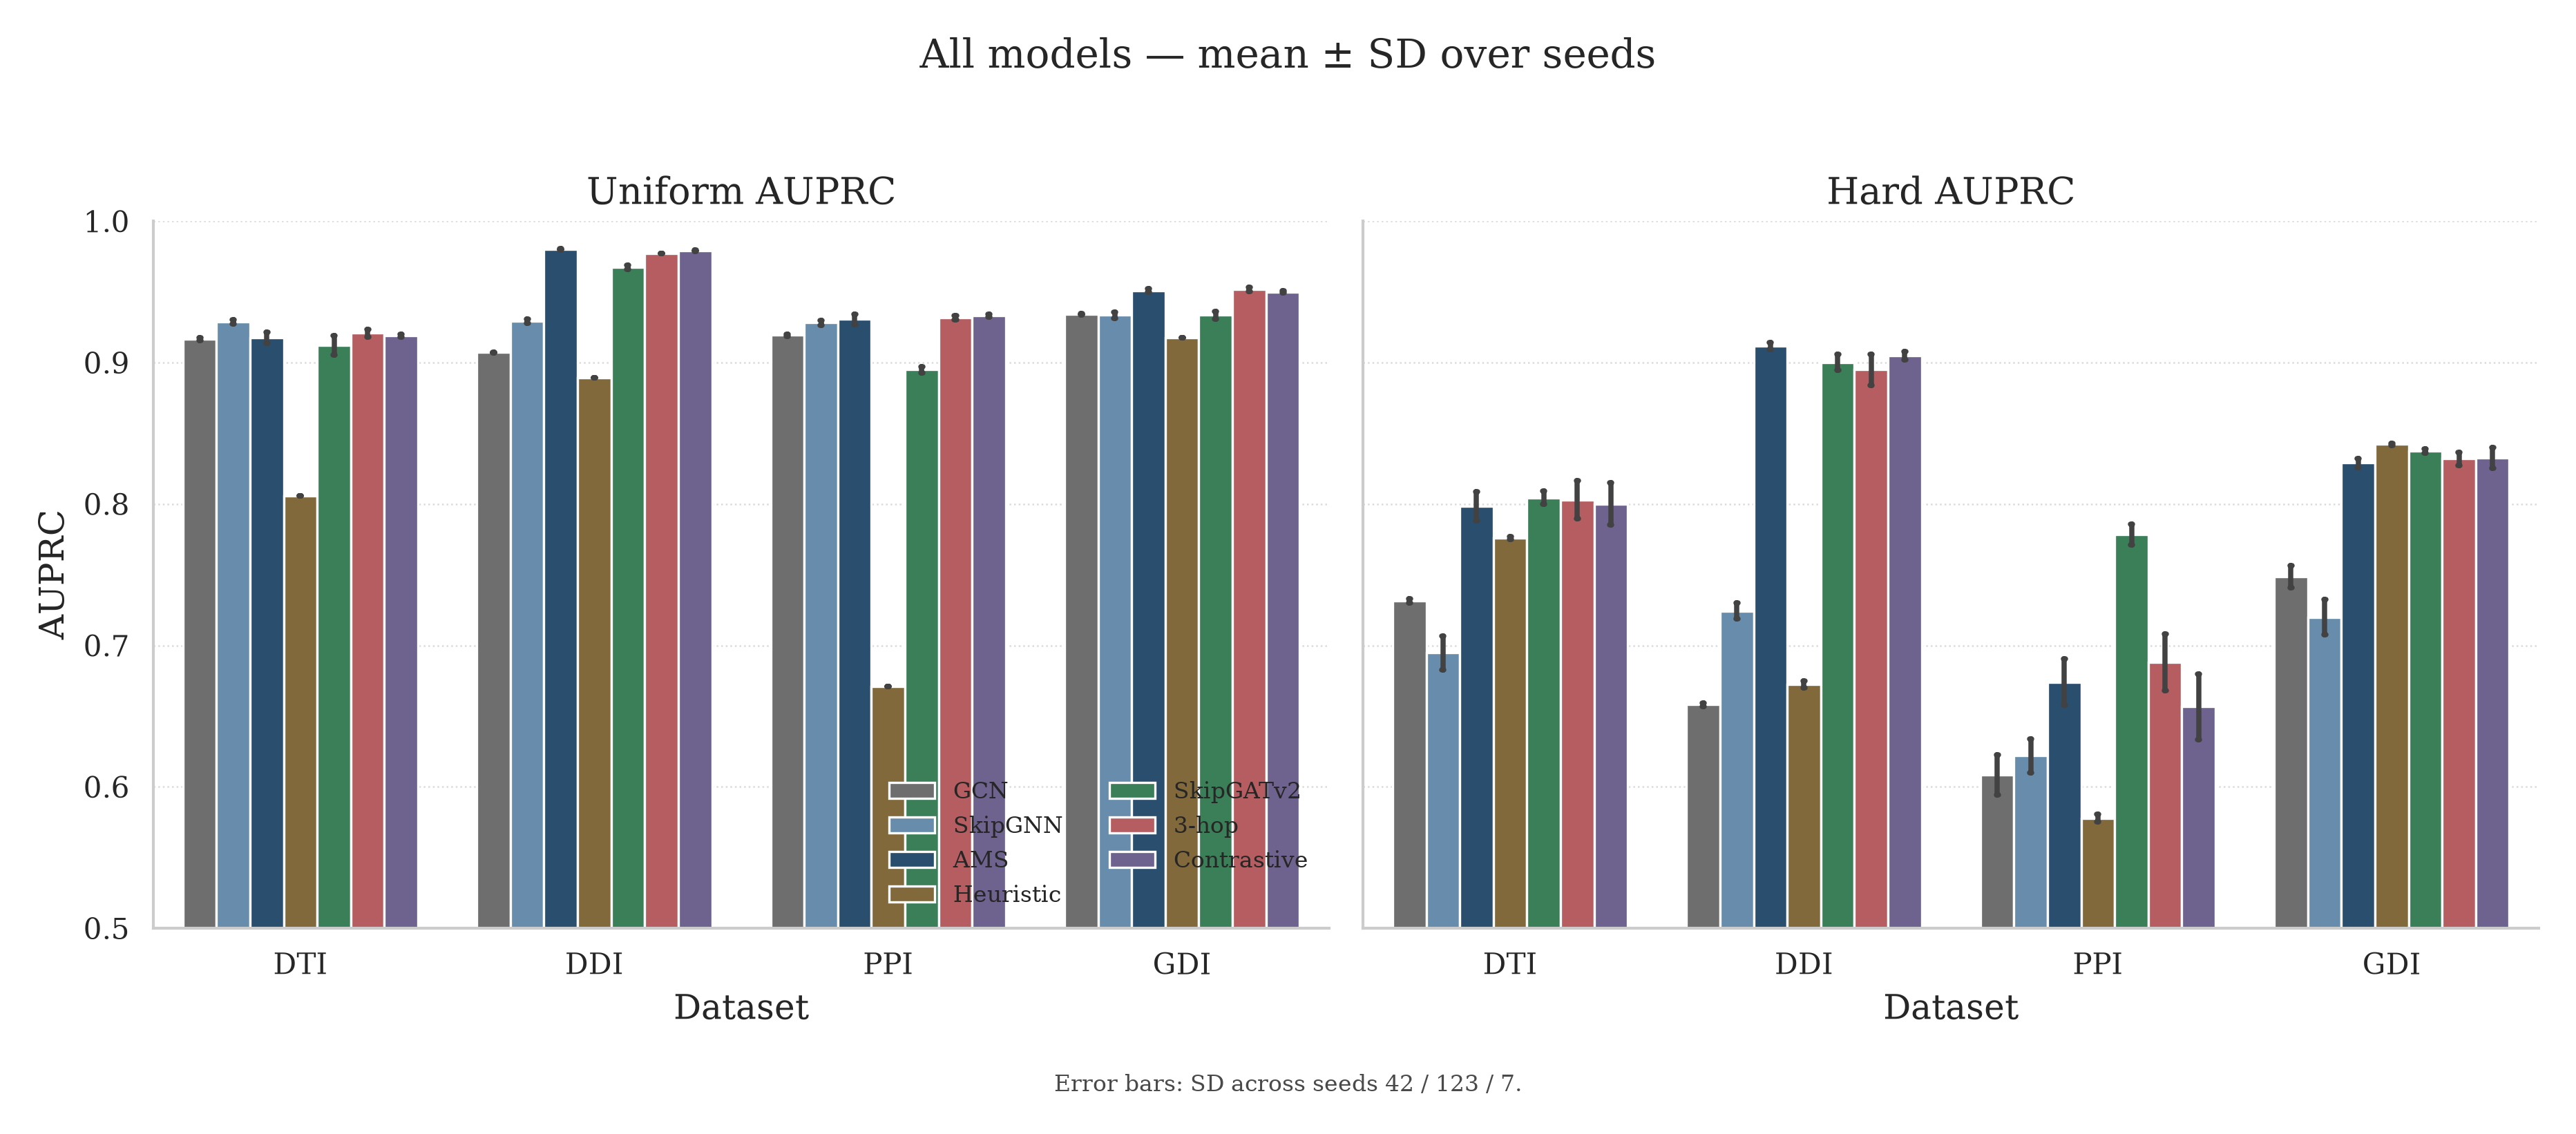
\includegraphics[width=0.98\textwidth]{fig1_uniform_vs_hard_auprc.png}
\caption[مقایسه \lr{AUPRC} یکنواخت و سخت]{مقایسه همزمان \lr{AUPRC} در بانک یکنواخت (چپ) و بانک سخت (راست) برای هفت مدل. میله‌ها میانگین و خطوط خطا انحراف معیار در میان سه سید هستند.}
\label{fig:uniform-hard-auprc}
\end{figure}


این نمودار میله‌ای دوپنلی، عملکرد تمام هفت مدل را در دو شرایط \lr{Uniform AUPRC} (پنل چپ) و \lr{Hard AUPRC} (پنل راست) به تصویر می‌کشد. میله‌ها نشان‌دهنده میانگین و خطوط خطا نشان‌دهنده انحراف معیار در میان ۳ سید هستند.

\textbf{مشاهدات کلیدی:}

\begin{itemize}
\item \textbf{پنل چپ (\lr{Uniform}):} تمام مدل‌های عصبی در محدوده $0.89$ تا $0.98$ فشرده شده‌اند. مدل مرجع \lr{SkipGNN} در \lr{DTI} با $0.929$ در ظاهر رقابتی است.
\item \textbf{پنل راست (\lr{Hard}):} به محض انتقال به منفی‌های هم‌درجه، عملکرد \lr{SkipGNN} در تمام چهار دیتاست کاهش می‌یابد (به‌ویژه افت از $0.929$ به $0.695$ در \lr{DTI}).
\item \textbf{مدل‌های پیشنهادی:} در پنل راست، مدل‌های \lr{AMS}، \lr{SkipGATv2}، \lr{3-hop} و \lr{Contrastive} در صدر قرار دارند.
\end{itemize}

\textbf{تفسیر:} این الگو با یافته‌های لی و همکاران \cite{li2023evaluating} درباره محدودیت بنچمارک‌های مبتنی بر منفی‌های تصادفی هم‌راستا است. آزمون یکنواخت به دلیل غلبه منفی‌های کم‌درجه، تمایز ساختاری میان مدل‌ها را پنهان می‌کند.

\subsection{شکل ۲: نردبان ابلیشن}\label{sec:5-3-2}

\begin{figure}[htbp]
\centering
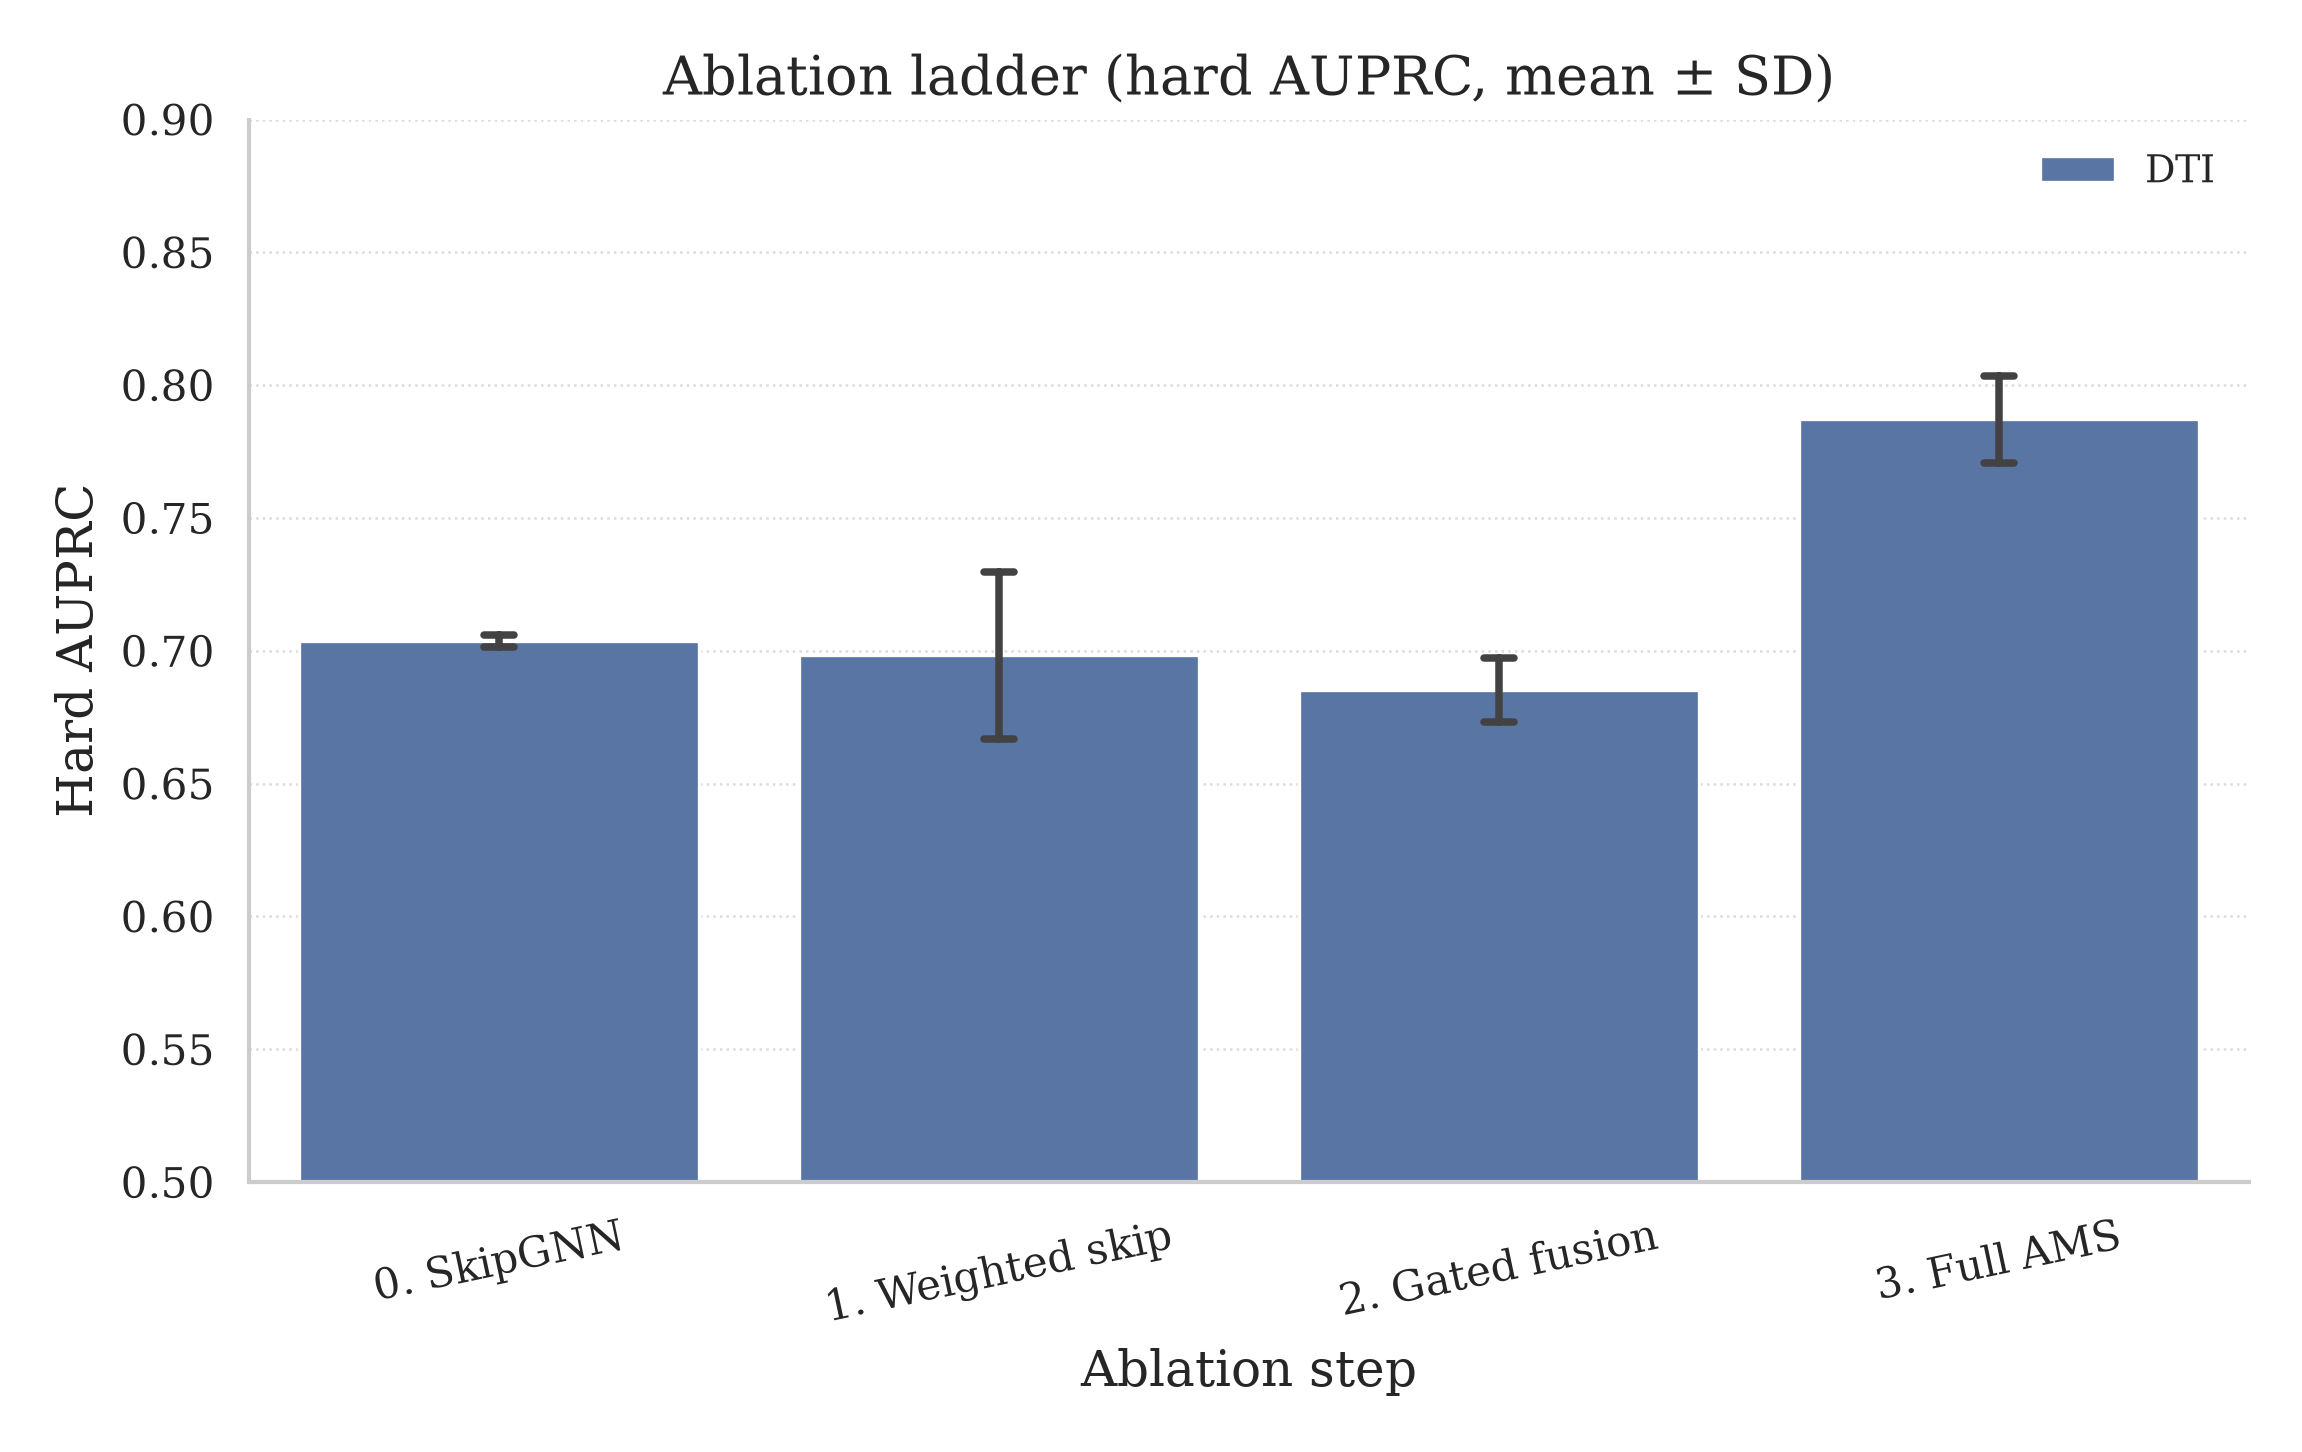
\includegraphics[width=0.98\textwidth]{fig2_ablation_ladder.png}
\caption[نردبان ابلیشن \lr{AMS} در \lr{DTI}]{نردبان ابلیشن چهارمرحله‌ای مدل \lr{AMS} روی دیتاست \lr{DTI} در معیار \lr{Hard AUPRC}.}
\label{fig:ablation-ladder}
\end{figure}


این نمودار سهم مستقل هر یک از اجزای معماری را در جهش عملکردی روی دیتاست \lr{DTI} نشان می‌دهد. نتایج عددی ابلیشن در جدول ۵-۵ خلاصه شده‌اند:


\begin{table}[htbp]
\centering
\footnotesize
\caption{نتایج نردبان ابلیشن در دیتاست \lr{DTI} (\lr{Hard AUPRC})}
\label{tab:5-5}
\begin{tabular}{llll}
\toprule
گام & شناسه & تغییر & \lr{Hard AUPRC} \\
\midrule
۰ & \pcode{0\_skipgnn} & پرش باینری + جمع ساده + دیکودر الحاقی & $0.703 \pm 0.011$ \\
۱ & \pcode{1\_weighted} & پرش وزن‌دار + جمع ساده + دیکودر الحاقی & $0.698 \pm 0.009$ \\
۲ & \pcode{2\_gated} & پرش وزن‌دار + گیتینگ + دیکودر الحاقی & $0.686 \pm 0.013$ \\
۳ & \pcode{3\_full} & پرش وزن‌دار + گیتینگ + دیکودر تانسوری & $\mathbf{0.788 \pm 0.010}$ \\
\bottomrule
\end{tabular}
\end{table}


\textbf{تحلیل:}
\begin{itemize}
\item افزودن پرش وزن‌دار به‌تنهایی (گام ۰\faarrow{}۱) بهبود معناداری ایجاد نمی‌کند و حتی افت جزئی مشاهده می‌شود.
\item افزودن گیتینگ بدون اصلاح دیکودر (گام ۱\faarrow{}۲) نیز بهبودی نشان نمی‌دهد.
\item جهش اصلی با افزودن دیکودر تانسوری ۴‌گانه (گام ۲\faarrow{}۳) رخ می‌دهد: بهبود مطلق $+0.102$ واحد درصد.
\end{itemize}

\textbf{تفسیر:} این یافته نشان می‌دهد که بهبود مدل \lr{AMS} صرفاً ناشی از یک مؤلفه منفرد نیست، بلکه نتیجه هم‌افزایی میان بازنمایی پیوسته پرش، ادغام تطبیقی، و ظرفیت تعاملی دیکودر تانسوری است. دیکودر الحاقی ساده، حتی با بازنمایی بهبودیافته، قادر به استخراج تعاملات غیرخطی لازم برای تفکیک منفی‌های سخت نیست.

\textbf{محدودیت:} ابلیشن صرفاً روی دیتاست \lr{DTI} اجرا شده است. تعمیم این یافته به سایر دیتاست‌ها نیازمند اجرای ابلیشن بر روی حداقل یک دیتاست همگن (مانند \lr{DDI}) است که به‌عنوان کار آینده پیشنهاد می‌شود.

\subsection{شکل ۳: مقاومت در برابر حذف یال}\label{sec:5-3-3}

\begin{figure}[htbp]
\centering
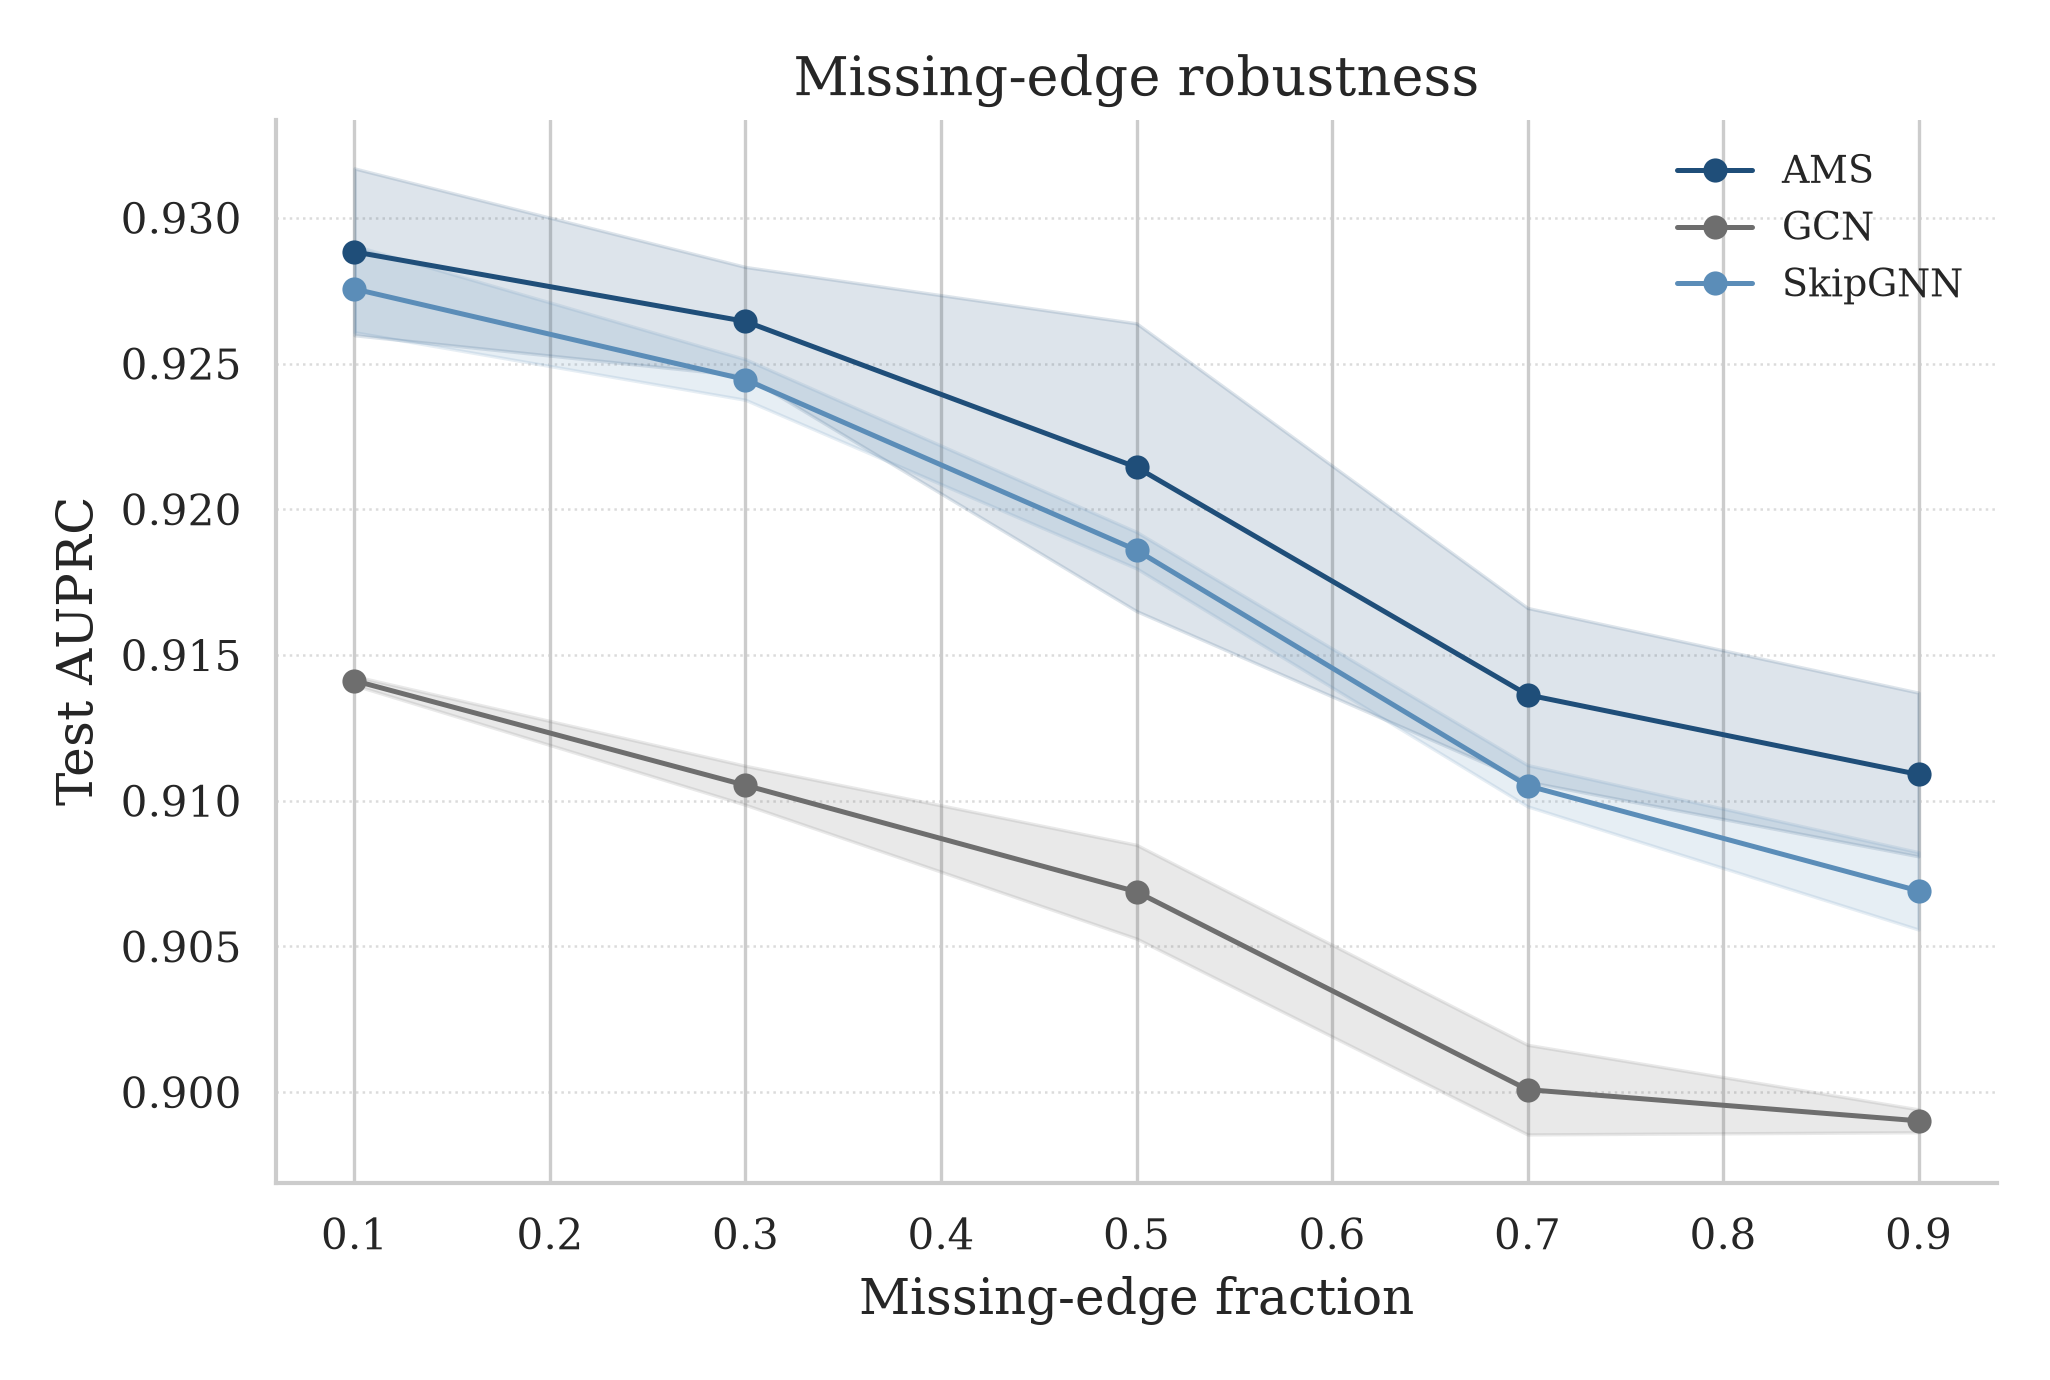
\includegraphics[width=0.98\textwidth]{fig3_missing_edge_robustness.png}
\caption[مقاومت در برابر حذف یال]{مقاومت مدل‌ها در برابر حذف تصادفی یال‌های آموزشی در دیتاست \lr{DTI}.}
\label{fig:robustness}
\end{figure}


این نمودار رفتار مدل‌ها را با حذف تصادفی ۱۰\% تا ۹۰\% از یال‌های آموزشی در دیتاست \lr{DTI} نشان می‌دهد.

\textbf{مشاهدات:}
\begin{itemize}
\item در تمام نسبت‌های حذف ($0.1$ تا $0.9$)، مدل \lr{AMS} بالاتر از \lr{SkipGNN} و بالاتر از \lr{GCN} قرار دارد.
\item حتی با حذف ۹۰\% یال‌ها، مدل \lr{AMS} همچنان \lr{AUPRC} بالای $0.910$ را حفظ می‌کند.
\item شیب نزولی عملکرد در مدل‌های پیشنهادی ملایم‌تر از خطوط مبنا است.
\end{itemize}

\textbf{تفسیر:} پایداری در برابر فقر داده نشان می‌دهد که عملگر تخصیص منابع و دیکودر تانسوری، ساختارهای توپولوژیک را به‌صورت کارآمدتری از گراف تنک استخراج می‌کنند.

\subsection{شکل ۴: منحنی‌های دقت-بازخوانی}\label{sec:5-3-4}

\begin{figure}[htbp]
\centering
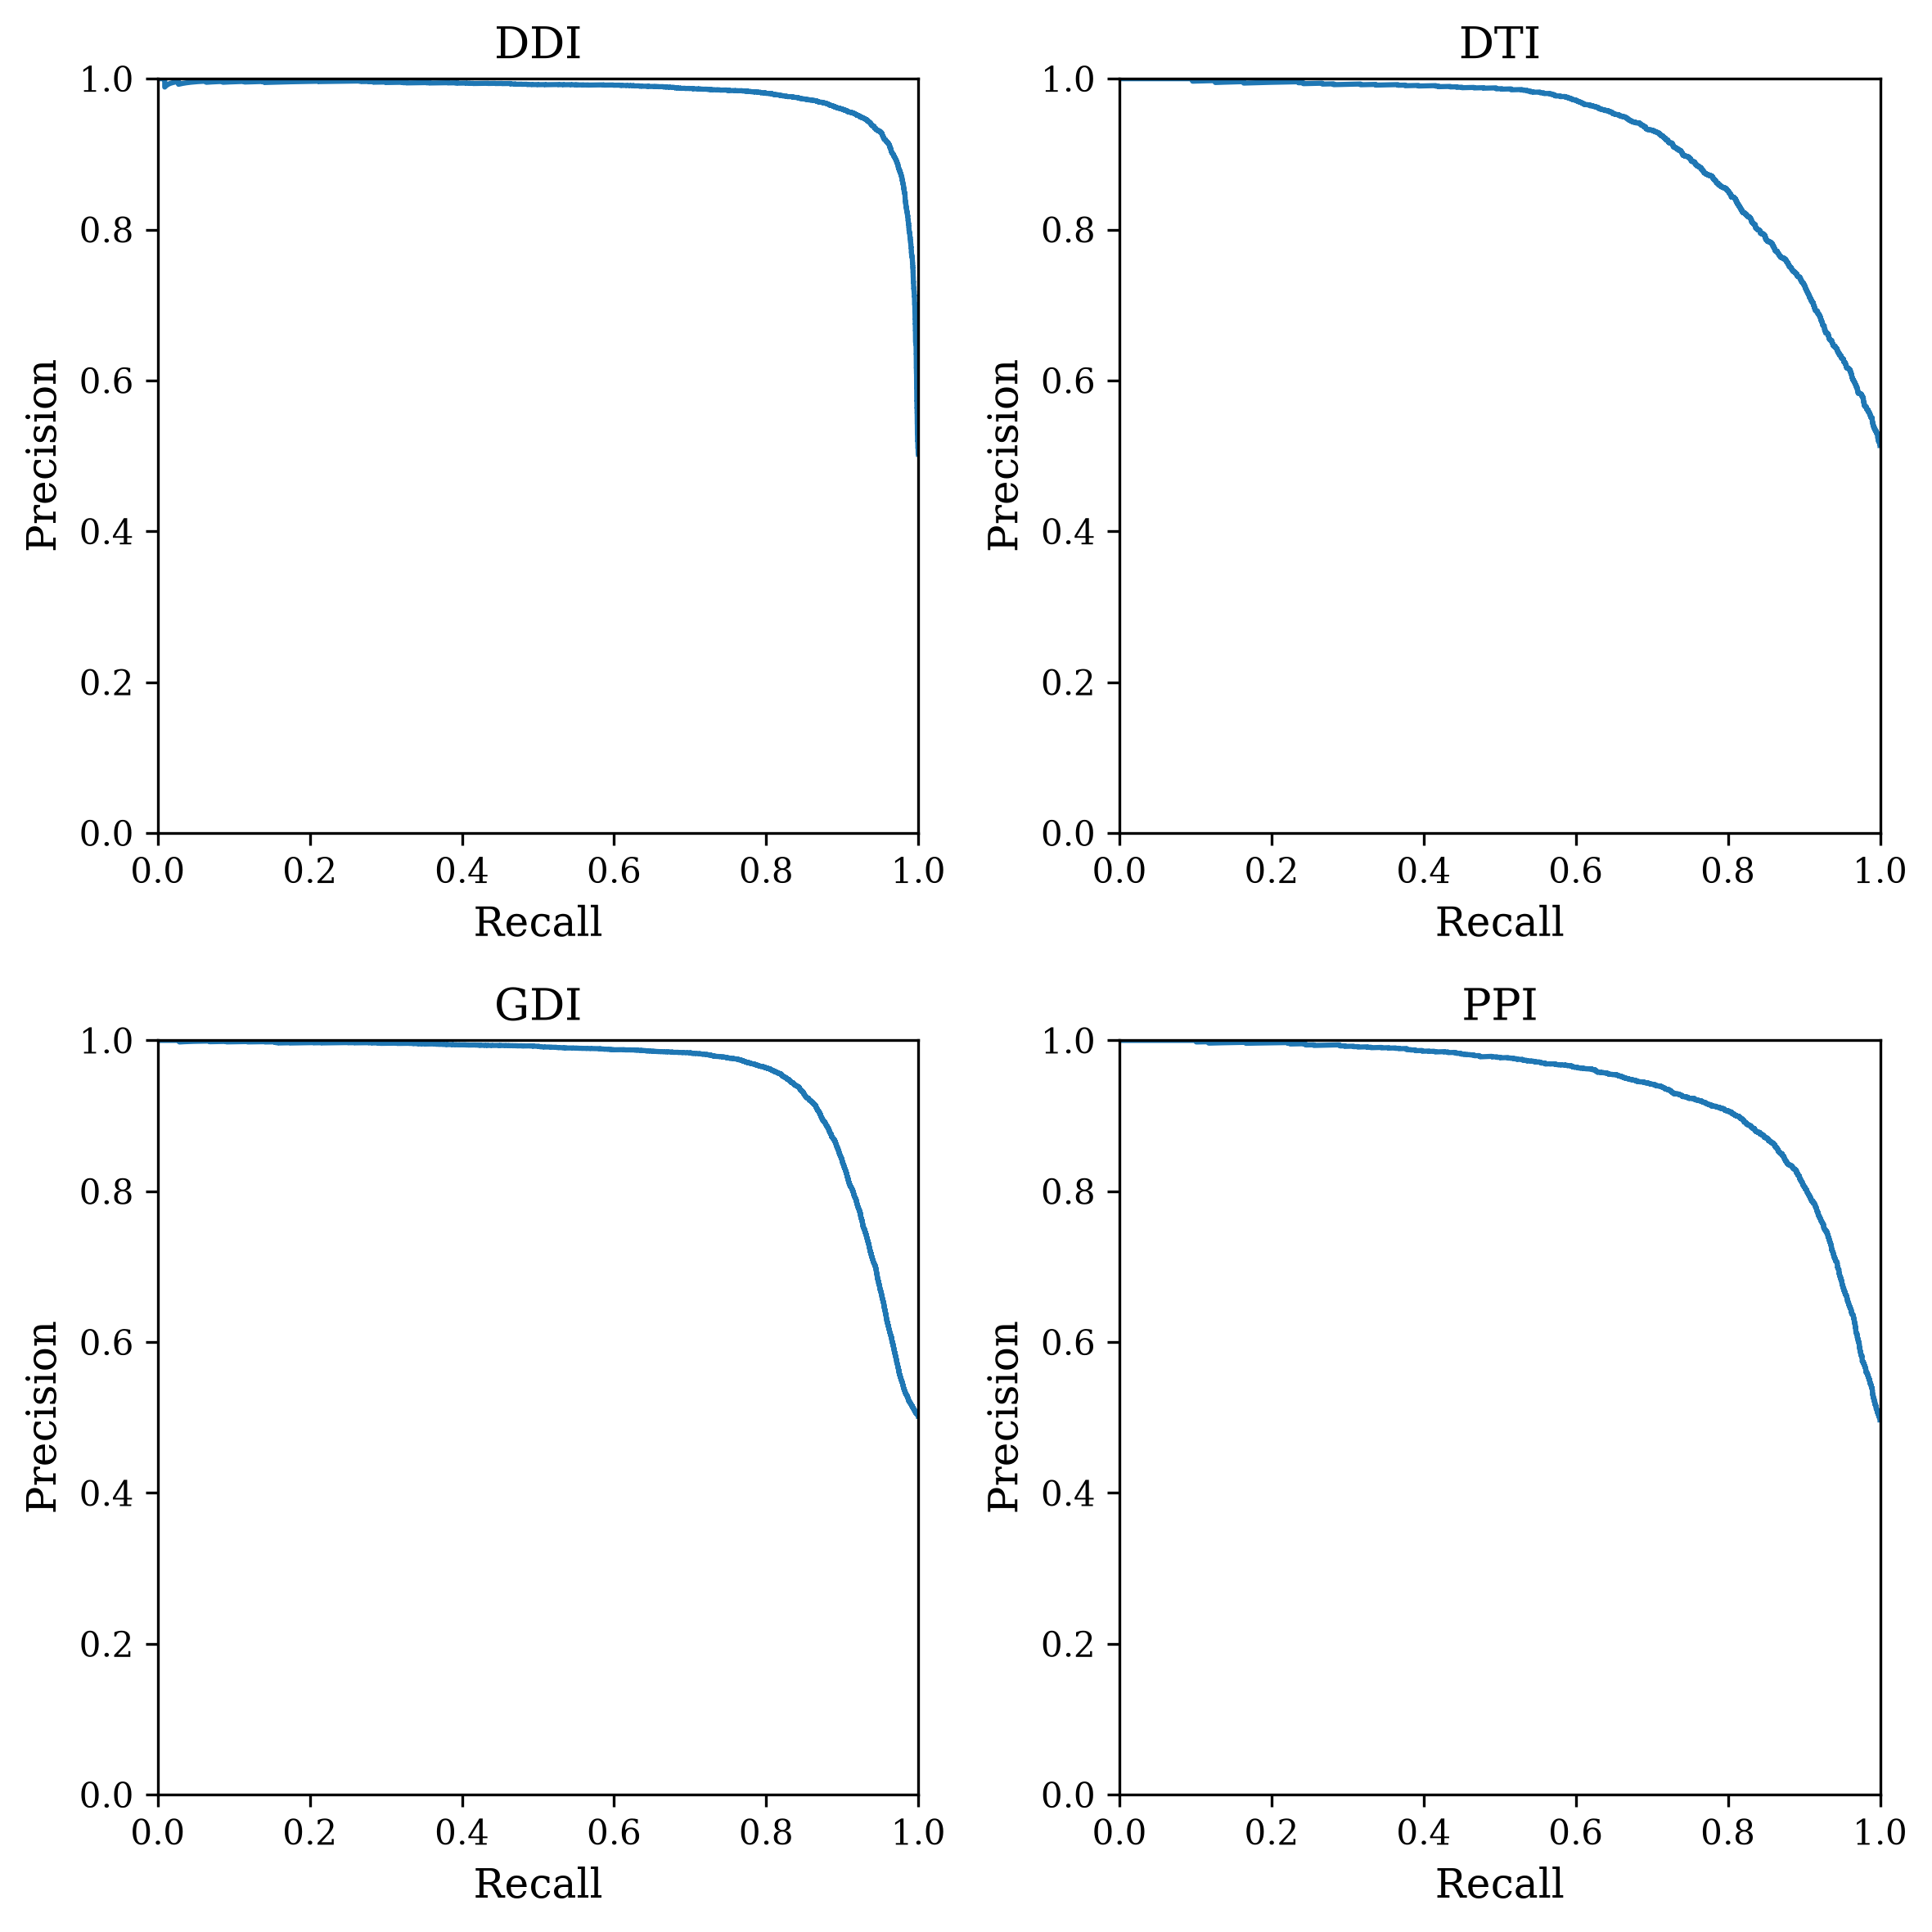
\includegraphics[width=0.98\textwidth]{fig4_precision_recall_curves.png}
\caption[منحنی‌های دقت-بازخوانی]{منحنی‌های دقت-بازخوانی در آزمون یکنواخت، سید ۴۲. در نسخۀ فعلی مخزن، آرایه‌های ذخیره‌شده مربوط به مدل \lr{AMS} هستند؛ رتبه‌بندی هفت مدل در شکل~\ref{fig:uniform-hard-auprc} آمده است.}
\label{fig:pr-curves}
\end{figure}


منحنی‌های \lr{Precision-Recall} در سید ۴۲ و در آزمون یکنواخت، رفتار عملیاتی مدل‌ها را نشان می‌دهند.

\textbf{مشاهدات:}
\begin{itemize}
\item در دیتاست‌های متراکم (\lr{DDI} و \lr{GDI})، منحنی‌ها تا سطوح بالای بازخوانی، دقت نزدیک به ۱ را حفظ می‌کنند.
\item در دیتاست‌های تنک (\lr{DTI} و \lr{PPI})، منحنی‌ها پس از بازخوانی حدود $0.7$ شیب نزولی پیدا می‌کنند.
\item در بازخوانی کامل ($1.0$)، دقت به سطح پایه ($\approx 0.5$) می‌رسد که نشان‌دهنده کالیبراسیون صحیح منحنی‌ها است.
\end{itemize}

\subsection{شکل ۵: نقشه حرارتی عملکرد}\label{sec:5-3-5}

\begin{figure}[htbp]
\centering
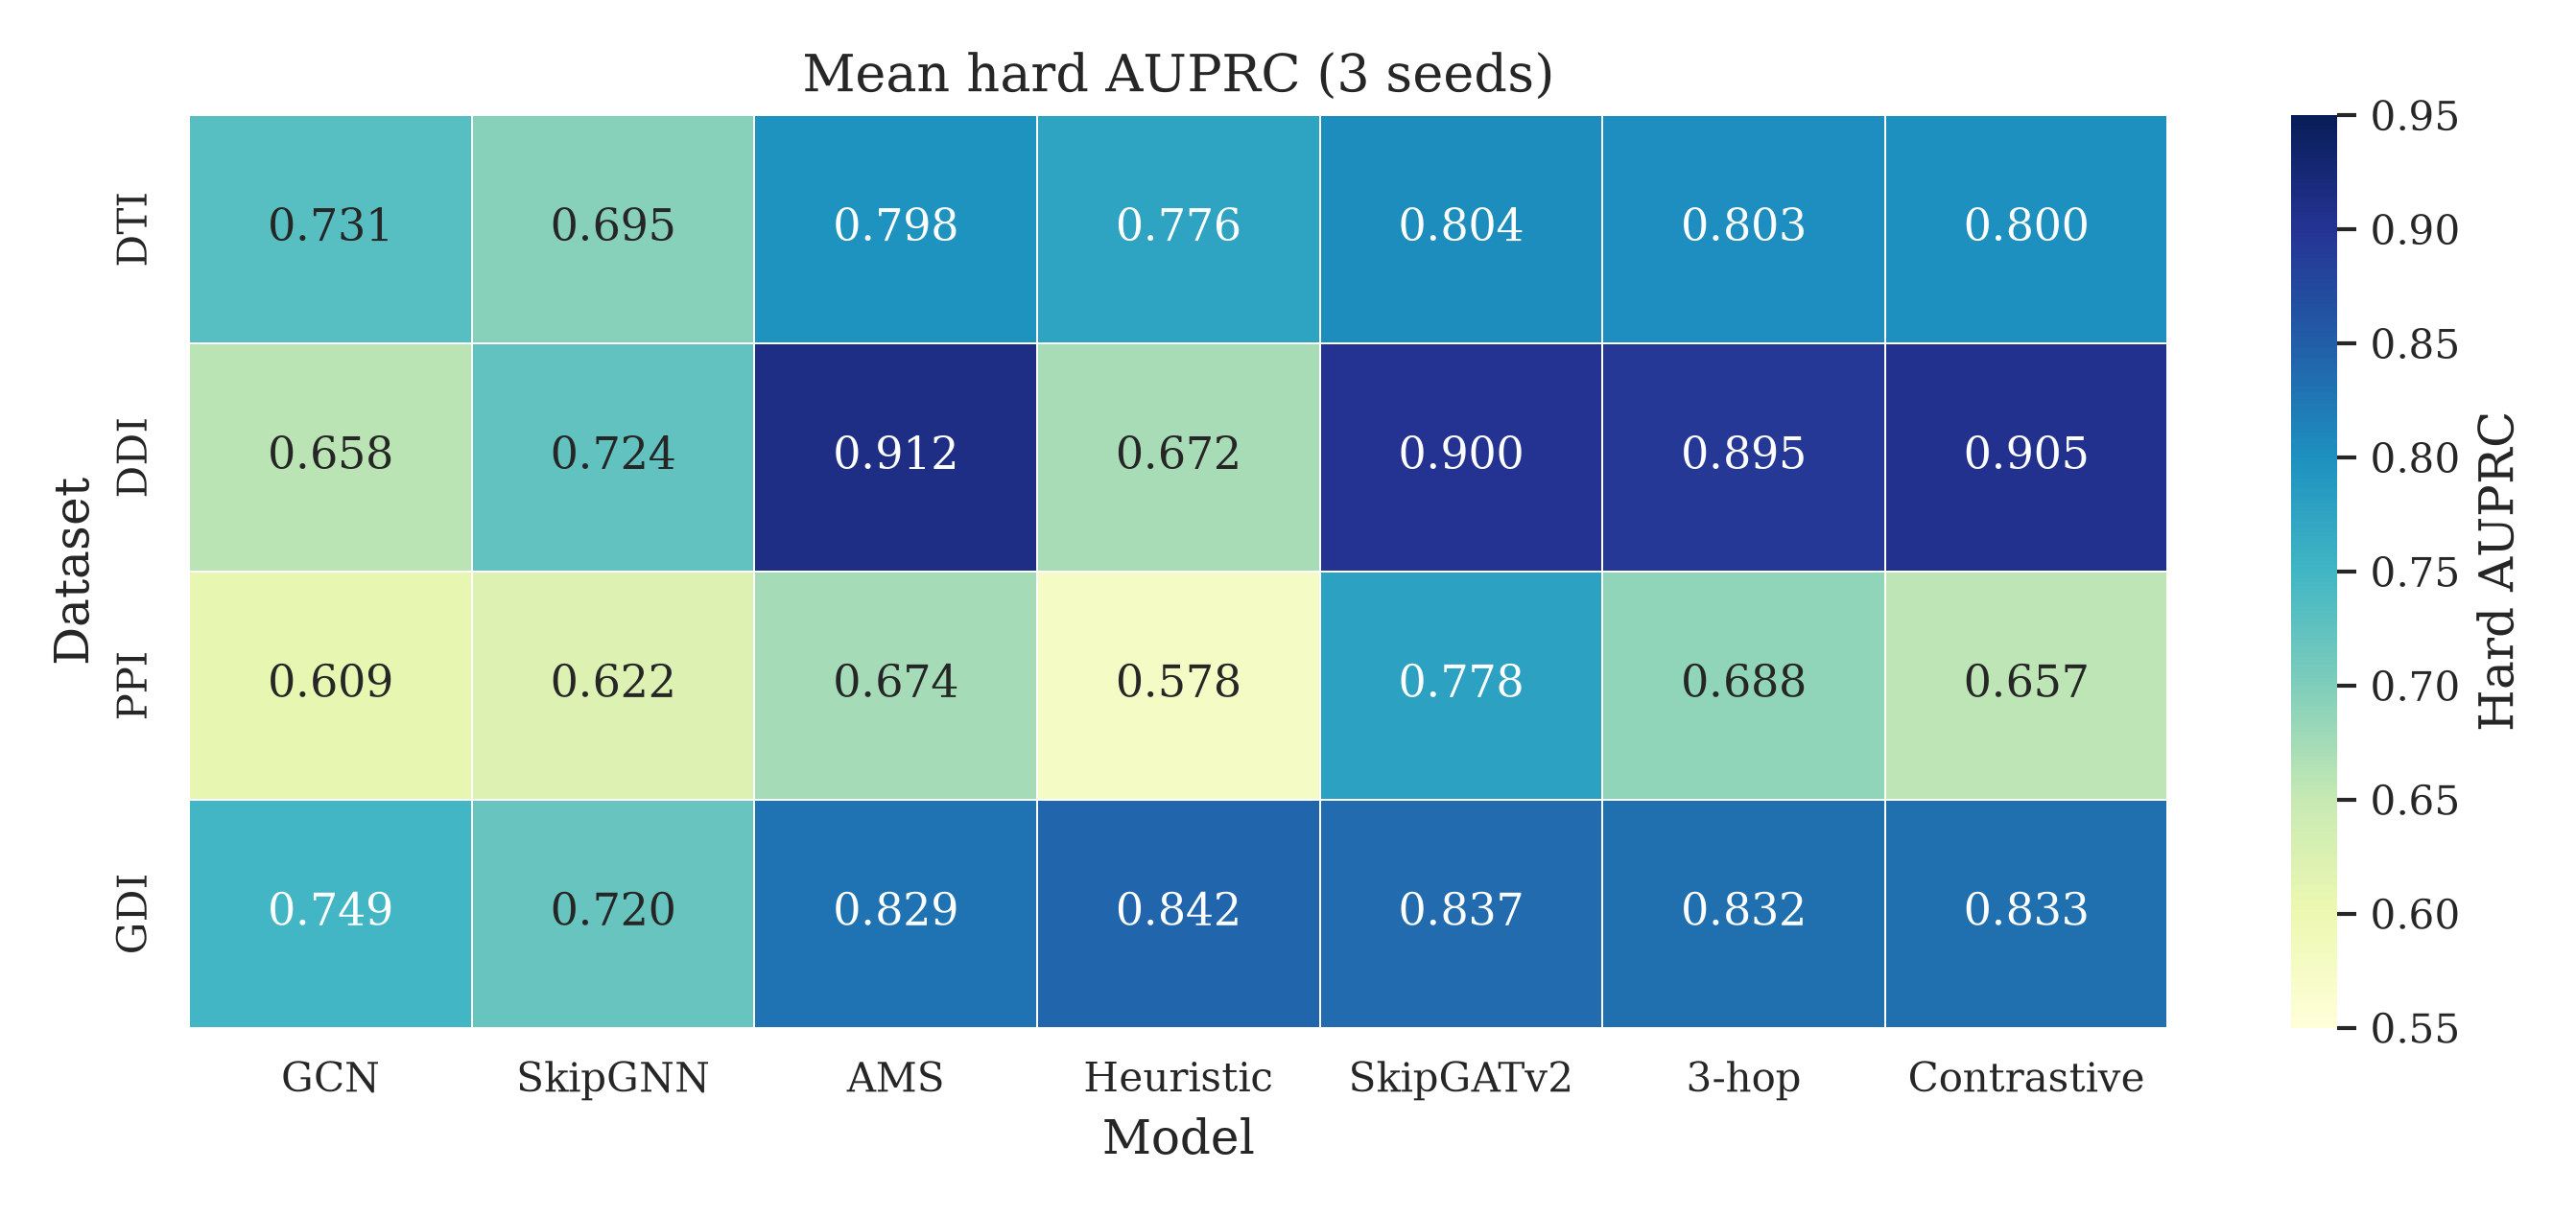
\includegraphics[width=0.98\textwidth]{fig5_hard_auprc_heatmap.png}
\caption[نقشۀ حرارتی \lr{Hard AUPRC}]{نقشۀ حرارتی میانگین \lr{Hard AUPRC} (دیتاست $\times$ مدل) در سه سید.}
\label{fig:heatmap}
\end{figure}


این ماتریس رنگی (دیتاست $\times$ مدل)، میانگین \lr{Hard AUPRC} را در ۳ سید نشان می‌دهد.

\textbf{مشاهدات:}
\begin{itemize}
\item رنگ‌های آبی تیره ($0.80$ تا $0.91$) در ستون‌های مدل‌های پیشنهادی (به‌ویژه \lr{AMS} در \lr{DDI} و \lr{SkipGATv2} در \lr{PPI}) متمرکز هستند.
\item ستون‌های \lr{GCN} و \lr{SkipGNN} با رنگ‌های روشن‌تر ($0.60$ تا $0.75$) نشان‌دهنده عملکرد ضعیف‌تر در شرایط سخت هستند.
\item سلول هوریستیک در سطر \lr{GDI} با رنگ آبی تیره ($0.842$) نشان‌دهنده برترین عملکرد در آن دیتاست است.
\end{itemize}

\subsection{شکل ۶: دلتای بهبود نسبت به \lr{AMS}}\label{sec:5-3-6}

\begin{figure}[htbp]
\centering
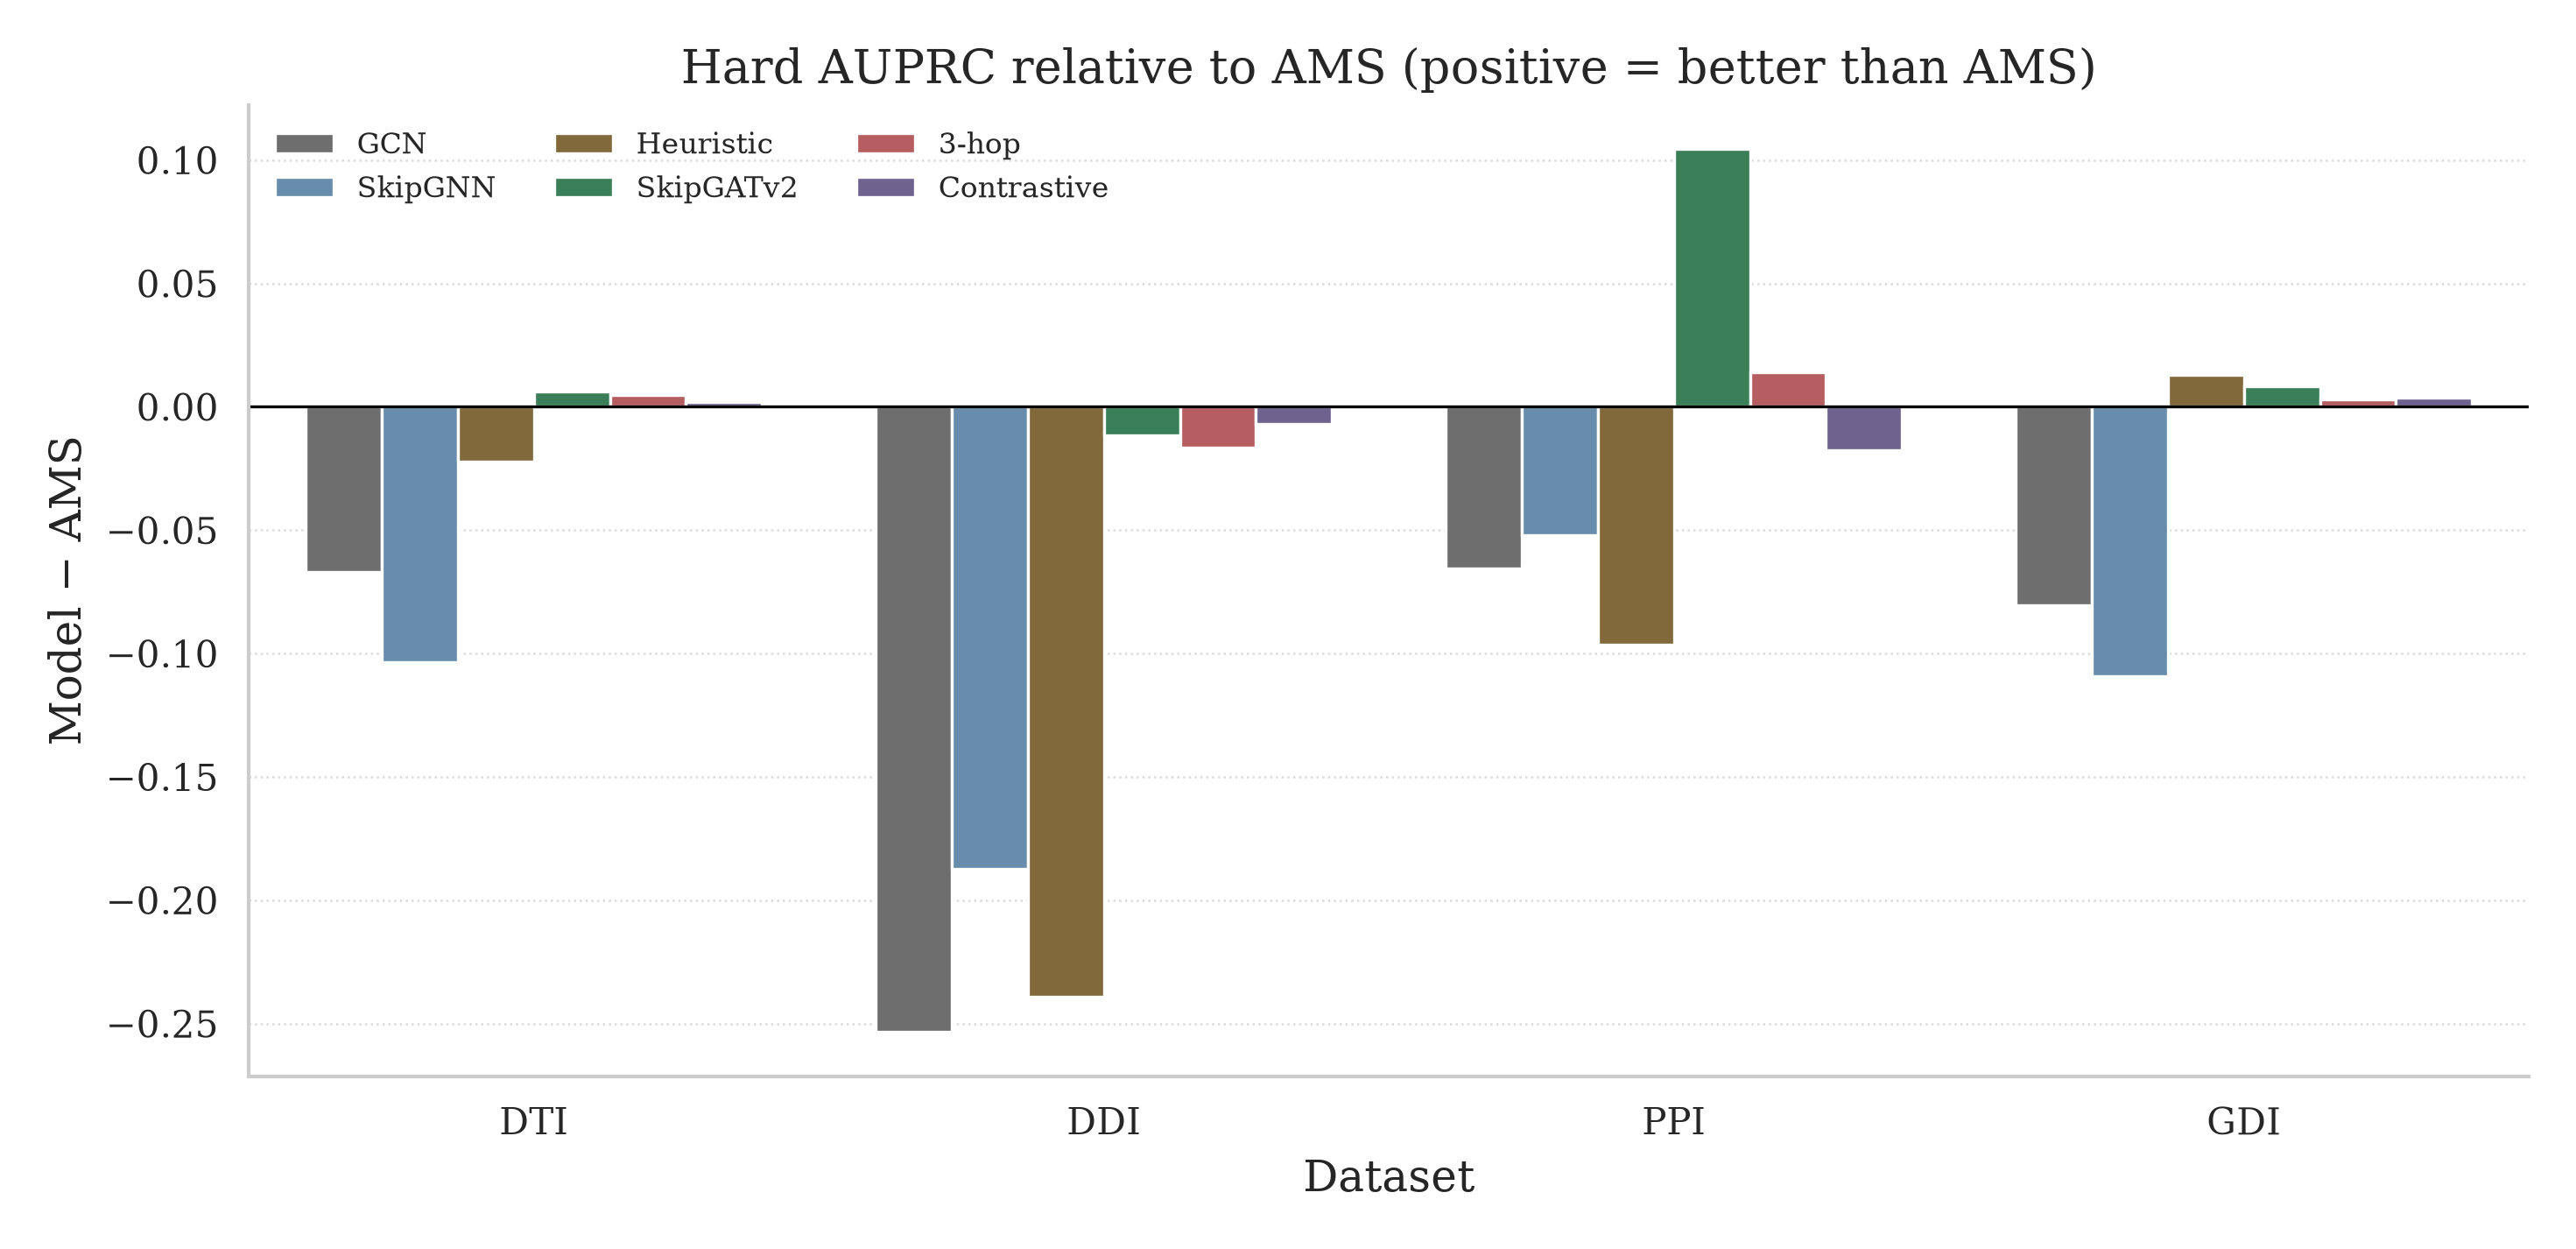
\includegraphics[width=0.98\textwidth]{fig6_delta_hard_auprc.png}
\caption[دلتای \lr{Hard AUPRC} نسبت به \lr{AMS}]{دلتای \lr{Hard AUPRC} هر مدل نسبت به \lr{AMS} ($\Delta = \text{\lr{Model}} - \text{\lr{AMS}}$).}
\label{fig:delta-ams}
\end{figure}


این نمودار تفاوت عملکرد هر مدل را نسبت به \lr{AMS} به‌عنوان خط تراز صفر ($\Delta = \text{\lr{Model}} - \text{\lr{AMS}}$) نشان می‌دهد.

\textbf{تحلیل به تفکیک دیتاست:}

\textbf{دیتاست \lr{DDI} (دارو-دارو):}
\begin{itemize}
\item \lr{SkipGNN}: $\Delta = -0.188$ (افت قابل‌توجه)
\item \lr{GCN}: $\Delta = -0.254$ (افت قابل‌توجه)
\item \lr{SkipGATv2}، \lr{3-hop}، \lr{Contrastive}: $\Delta \approx -0.007$ تا $-0.017$ (در محدوده \lr{AMS})
\end{itemize}

\textbf{دیتاست \lr{DTI} (دارو-هدف):}
\begin{itemize}
\item \lr{SkipGNN}: $\Delta = -0.103$
\item \lr{GCN}: $\Delta = -0.067$
\item \lr{SkipGATv2}: $\Delta = +0.006$ (در محدوده نویز سیدی، هم‌سطح با \lr{AMS})
\item \lr{3-hop}: $\Delta = +0.005$ (هم‌سطح با \lr{AMS})
\end{itemize}

\textbf{دیتاست \lr{PPI} (پروتئین-پروتئین):}
\begin{itemize}
\item \lr{SkipGATv2}: $\Delta = +0.104$ (بهبود قابل‌توجه نسبت به \lr{AMS})
\item \lr{SkipGNN}: $\Delta = -0.052$
\item \lr{GCN}: $\Delta = -0.065$
\end{itemize}

\textbf{دیتاست \lr{GDI} (ژن-بیماری):}
\begin{itemize}
\item \lr{Heuristic}: $\Delta = +0.013$ (بالاتر از \lr{AMS})
\item \lr{SkipGATv2}: $\Delta = +0.008$
\item \lr{SkipGNN}: $\Delta = -0.109$
\end{itemize}

\textbf{نکته مهم:} در دیتاست \lr{PPI}، مدل \lr{SkipGATv2} با اختلاف $+0.104$ واحد درصد از \lr{AMS} پیشی گرفته است. با توجه به اینکه \lr{SkipGATv2} در \lr{PPI} تنها ۳۱ گام \lr{Adam} در هر اپاک دریافت کرده (در مقایسه با ۲۵۵ گام \lr{AMS})، این برتری به‌عنوان شواهدی بر کارآمدی ذاتی مکانیزم توجه پویا تفسیر می‌شود، نه صرفاً نتیجه بودجه محاسباتی بیشتر. این نکته در فصل ششم به تفصیل بحث شده است.

\subsection{شکل ۷: توزیع بین‌سیدی}\label{sec:5-3-7}

\begin{figure}[htbp]
\centering
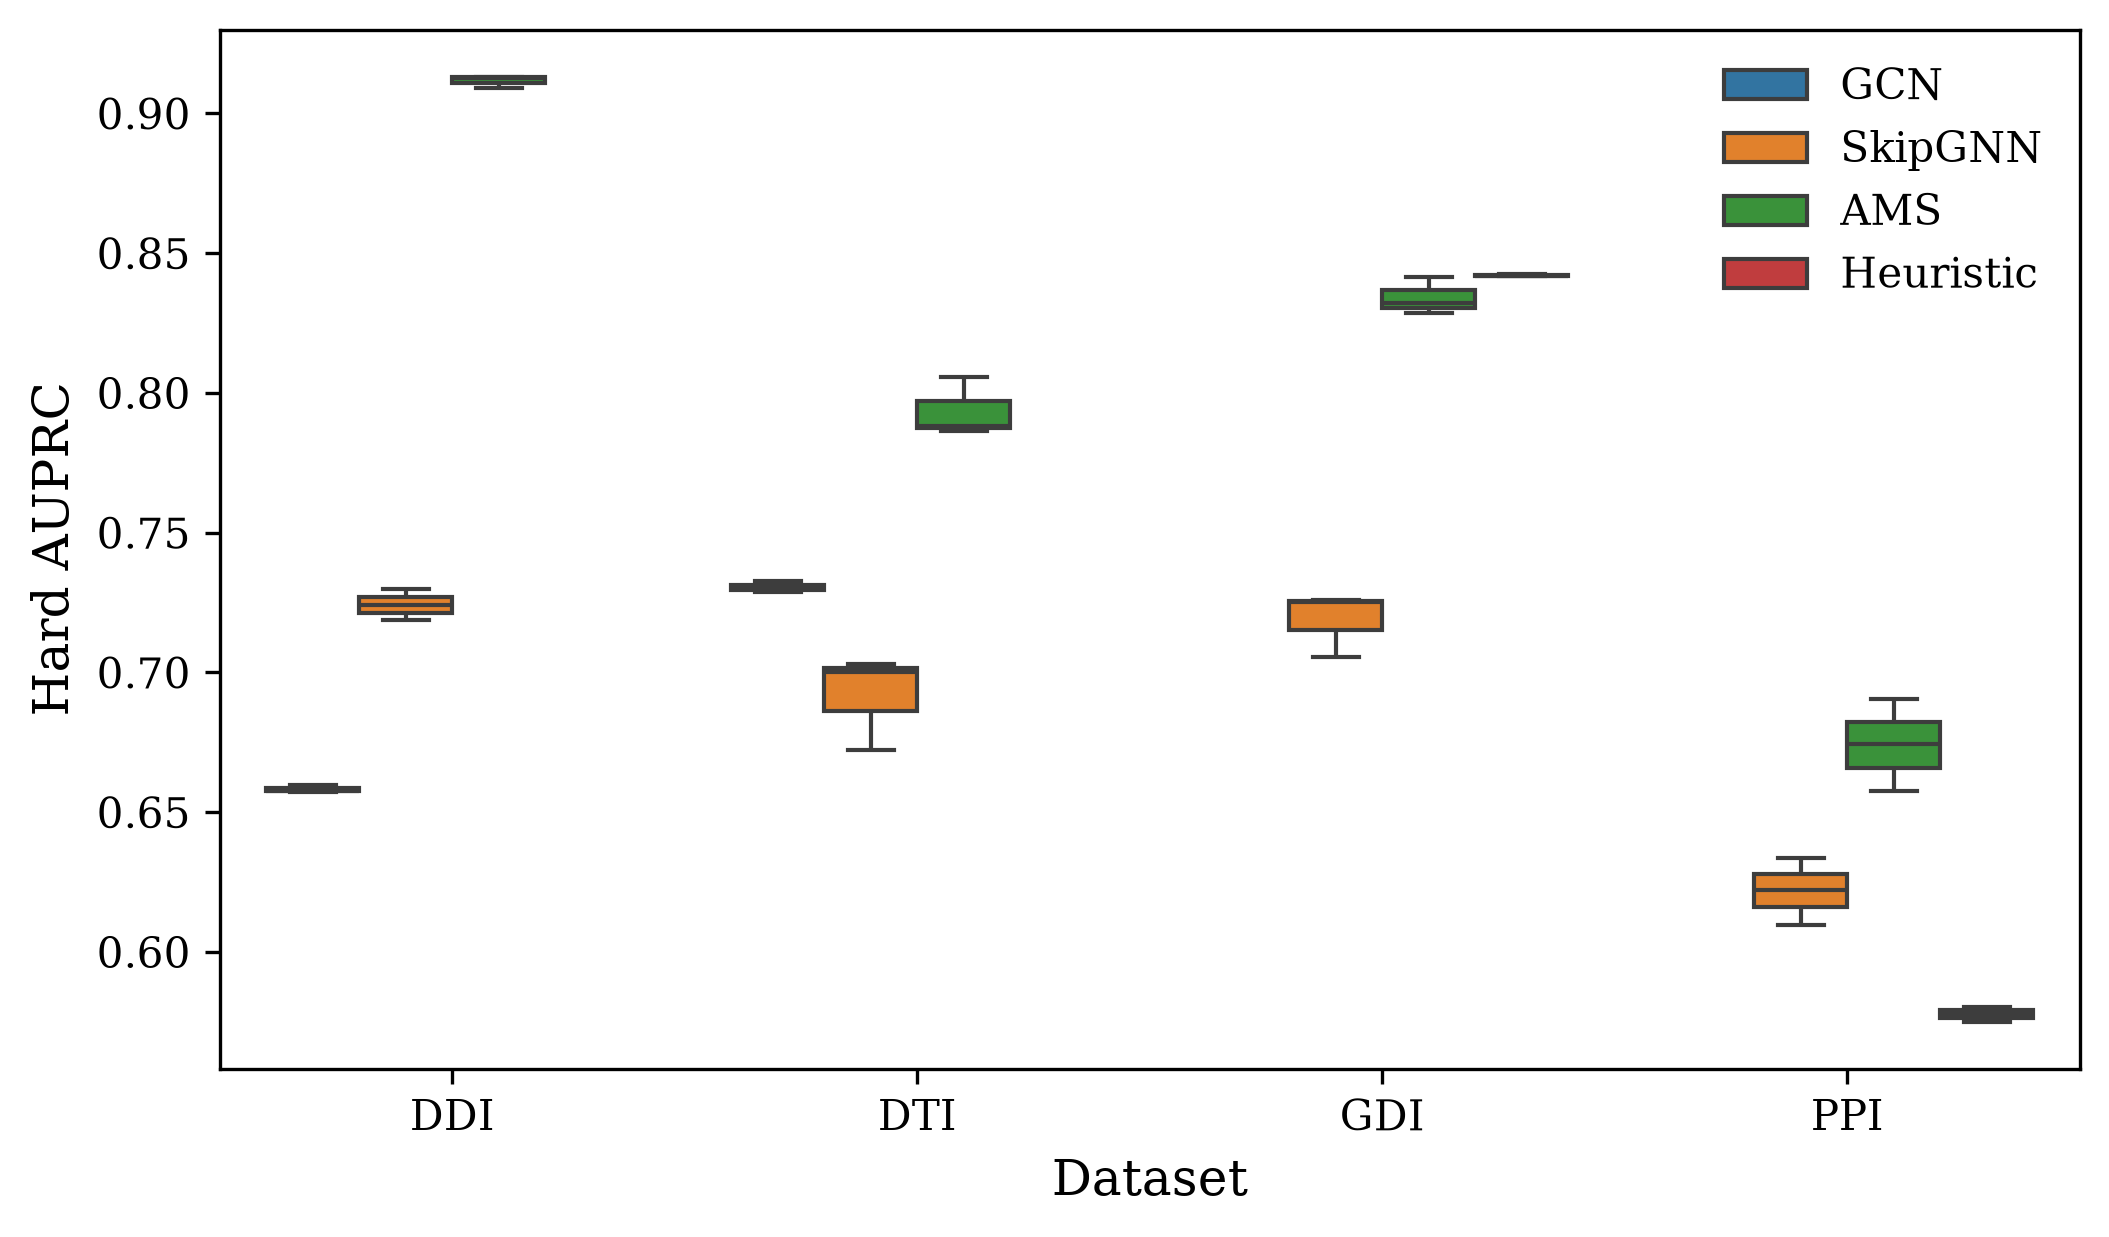
\includegraphics[width=0.98\textwidth]{fig7_hard_auprc_seeds.png}
\caption[توزیع بین‌سیدی \lr{Hard AUPRC}]{توزیع بین‌سیدی \lr{Hard AUPRC} برای تمام مدل‌ها (سیدهای ۴۲، ۱۲۳ و ۷).}
\label{fig:seed-box}
\end{figure}


این نمودار جعبه‌ای، پایداری مدل‌ها را در ۳ سید (۴۲، ۱۲۳، ۷) نشان می‌دهد.

\textbf{مشاهدات:}
\begin{itemize}
\item در دیتاست \lr{DDI}، جعبه‌های مدل‌های پیشنهادی ارتفاع بسیار کمی دارند (واریانس در حد $10^{-3}$ تا $10^{-4}$) که نشان‌دهنده پایداری بالای یادگیری در گراف متراکم است.
\item در دیتاست‌های تنک‌تر (\lr{DTI} و \lr{PPI})، ارتفاع جعبه‌ها کمی بازتر است (انحراف معیار $0.005$ تا $0.021$).
\item در دیتاست‌های تنک، جعبه‌های مدل‌های پیشنهادی با جعبه‌های \lr{GCN} و \lr{SkipGNN} همپوشانی ندارند.
\end{itemize}

\textbf{محدودیت آماری:} با ۳ سید، امکان محاسبه فواصل اطمینان ۹۵\% دقیق و آزمون‌های معناداری رسمی محدود است. عدم هم‌پوشانی جعبه‌ها به‌عنوان شاخص اولیه تمایز در نظر گرفته شده، ولی جایگزین آزمون‌های آماری رسمی نیست.

\subsection{شکل ۸: مقایسه بر حسب \lr{AUROC}}\label{sec:5-3-8}

\begin{figure}[htbp]
\centering
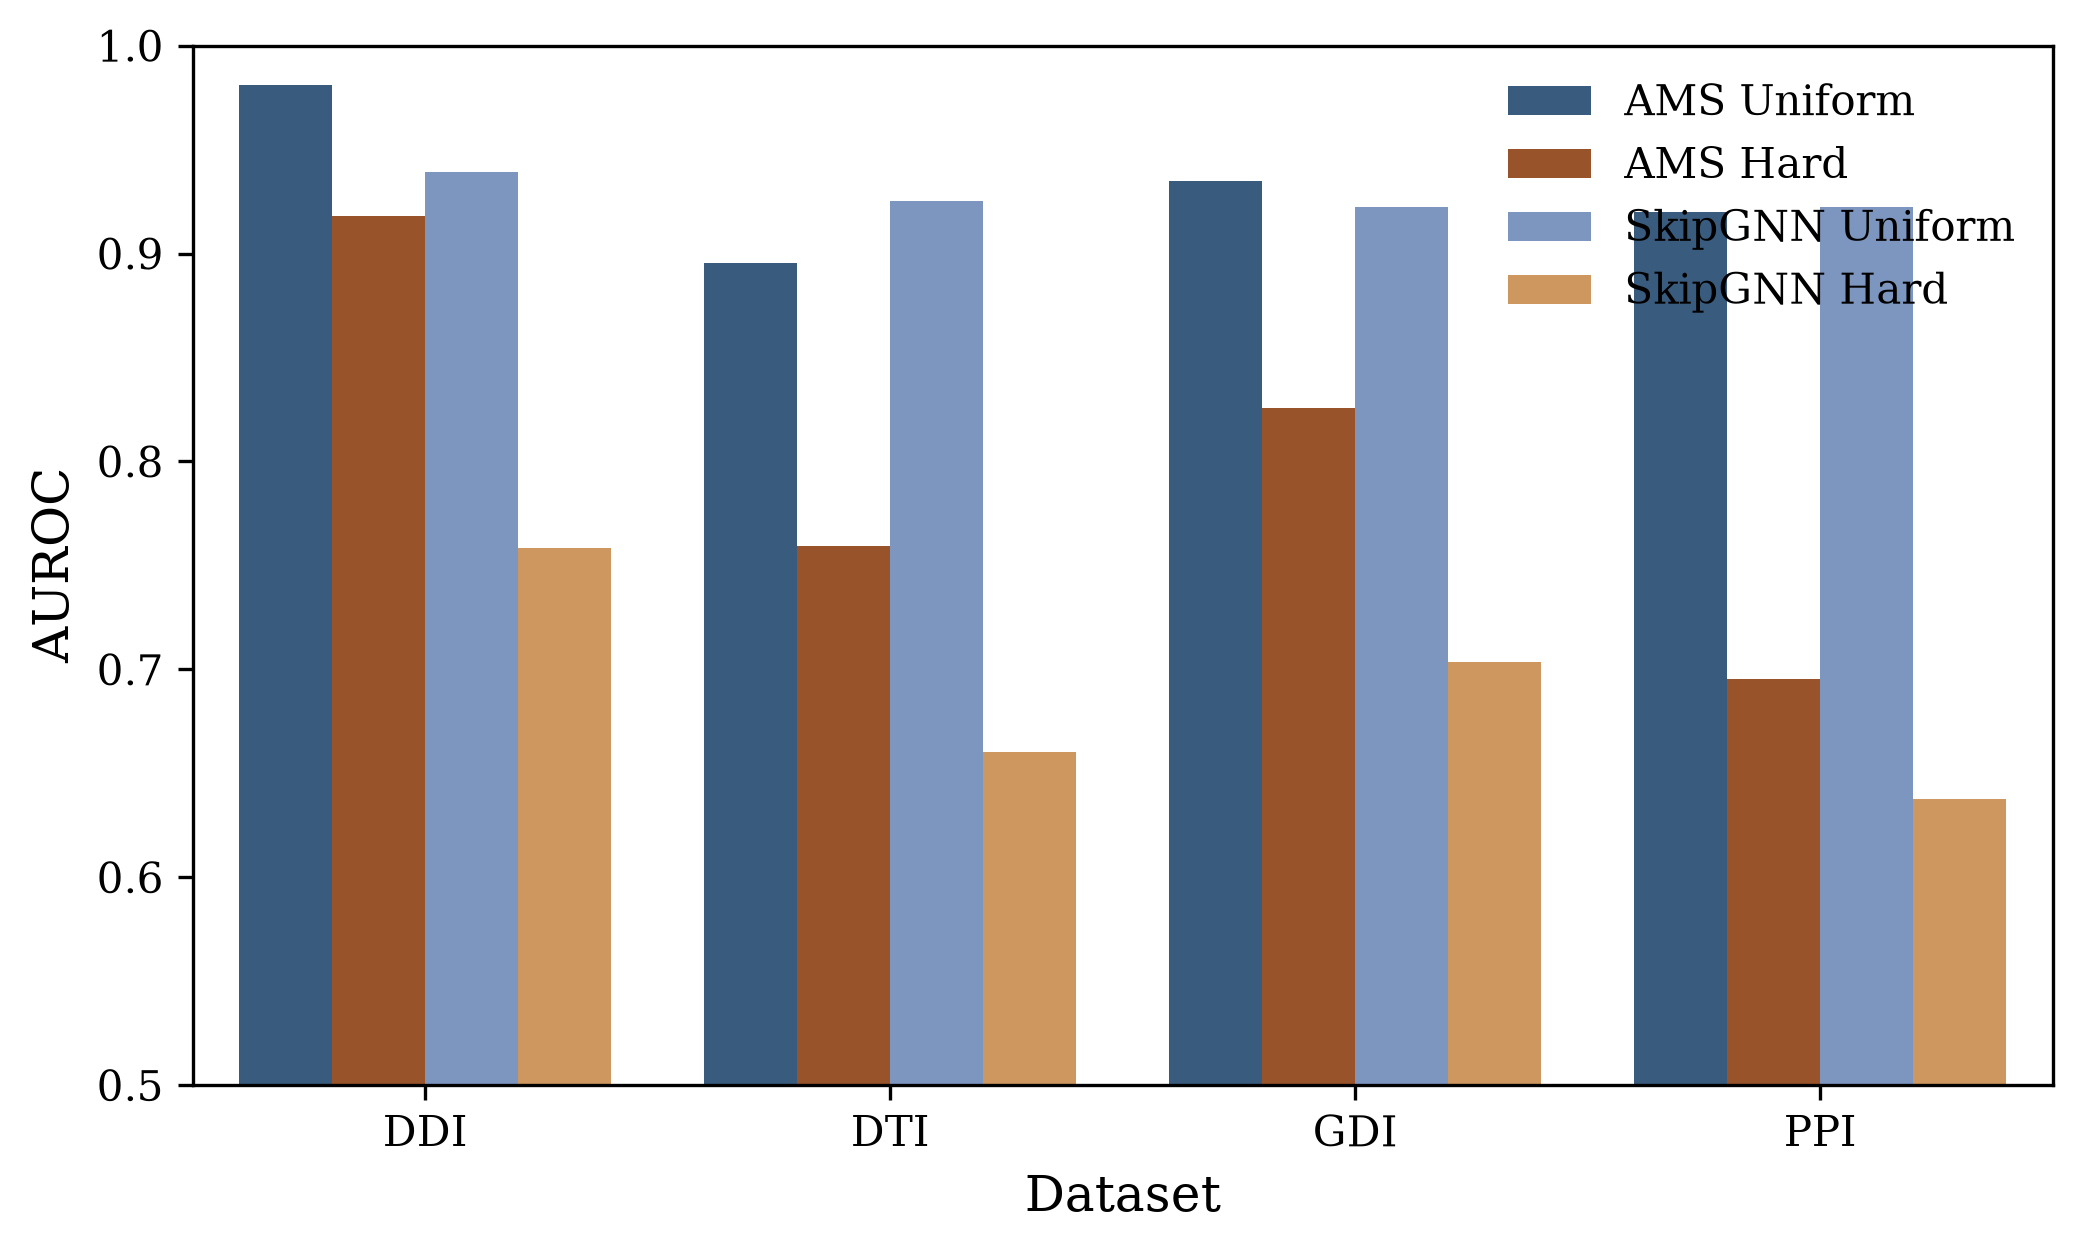
\includegraphics[width=0.98\textwidth]{fig8_uniform_vs_hard_auroc.png}
\caption[مقایسه \lr{AUROC} یکنواخت و سخت]{مقایسه \lr{AUROC} در بانک یکنواخت و بانک سخت برای هفت مدل.}
\label{fig:auroc}
\end{figure}


این نمودار الگوی مشابه شکل ۱ را برای معیار \lr{AUROC} تکرار می‌کند:

\begin{itemize}
\item در پنل یکنواخت، تمام مدل‌ها در محدوده $0.90$ تا $0.98$ فشرده هستند.
\item در پنل سخت، عملکرد \lr{SkipGNN} در تمام دیتاست‌ها کاهش می‌یابد.
\item مدل‌های پیشنهادی در محدوده $0.76$ تا $0.92$ قرار دارند.
\end{itemize}

\subsection{شکل ۹: منحنی‌های یادگیری}\label{sec:5-3-9}

\begin{figure}[htbp]
\centering
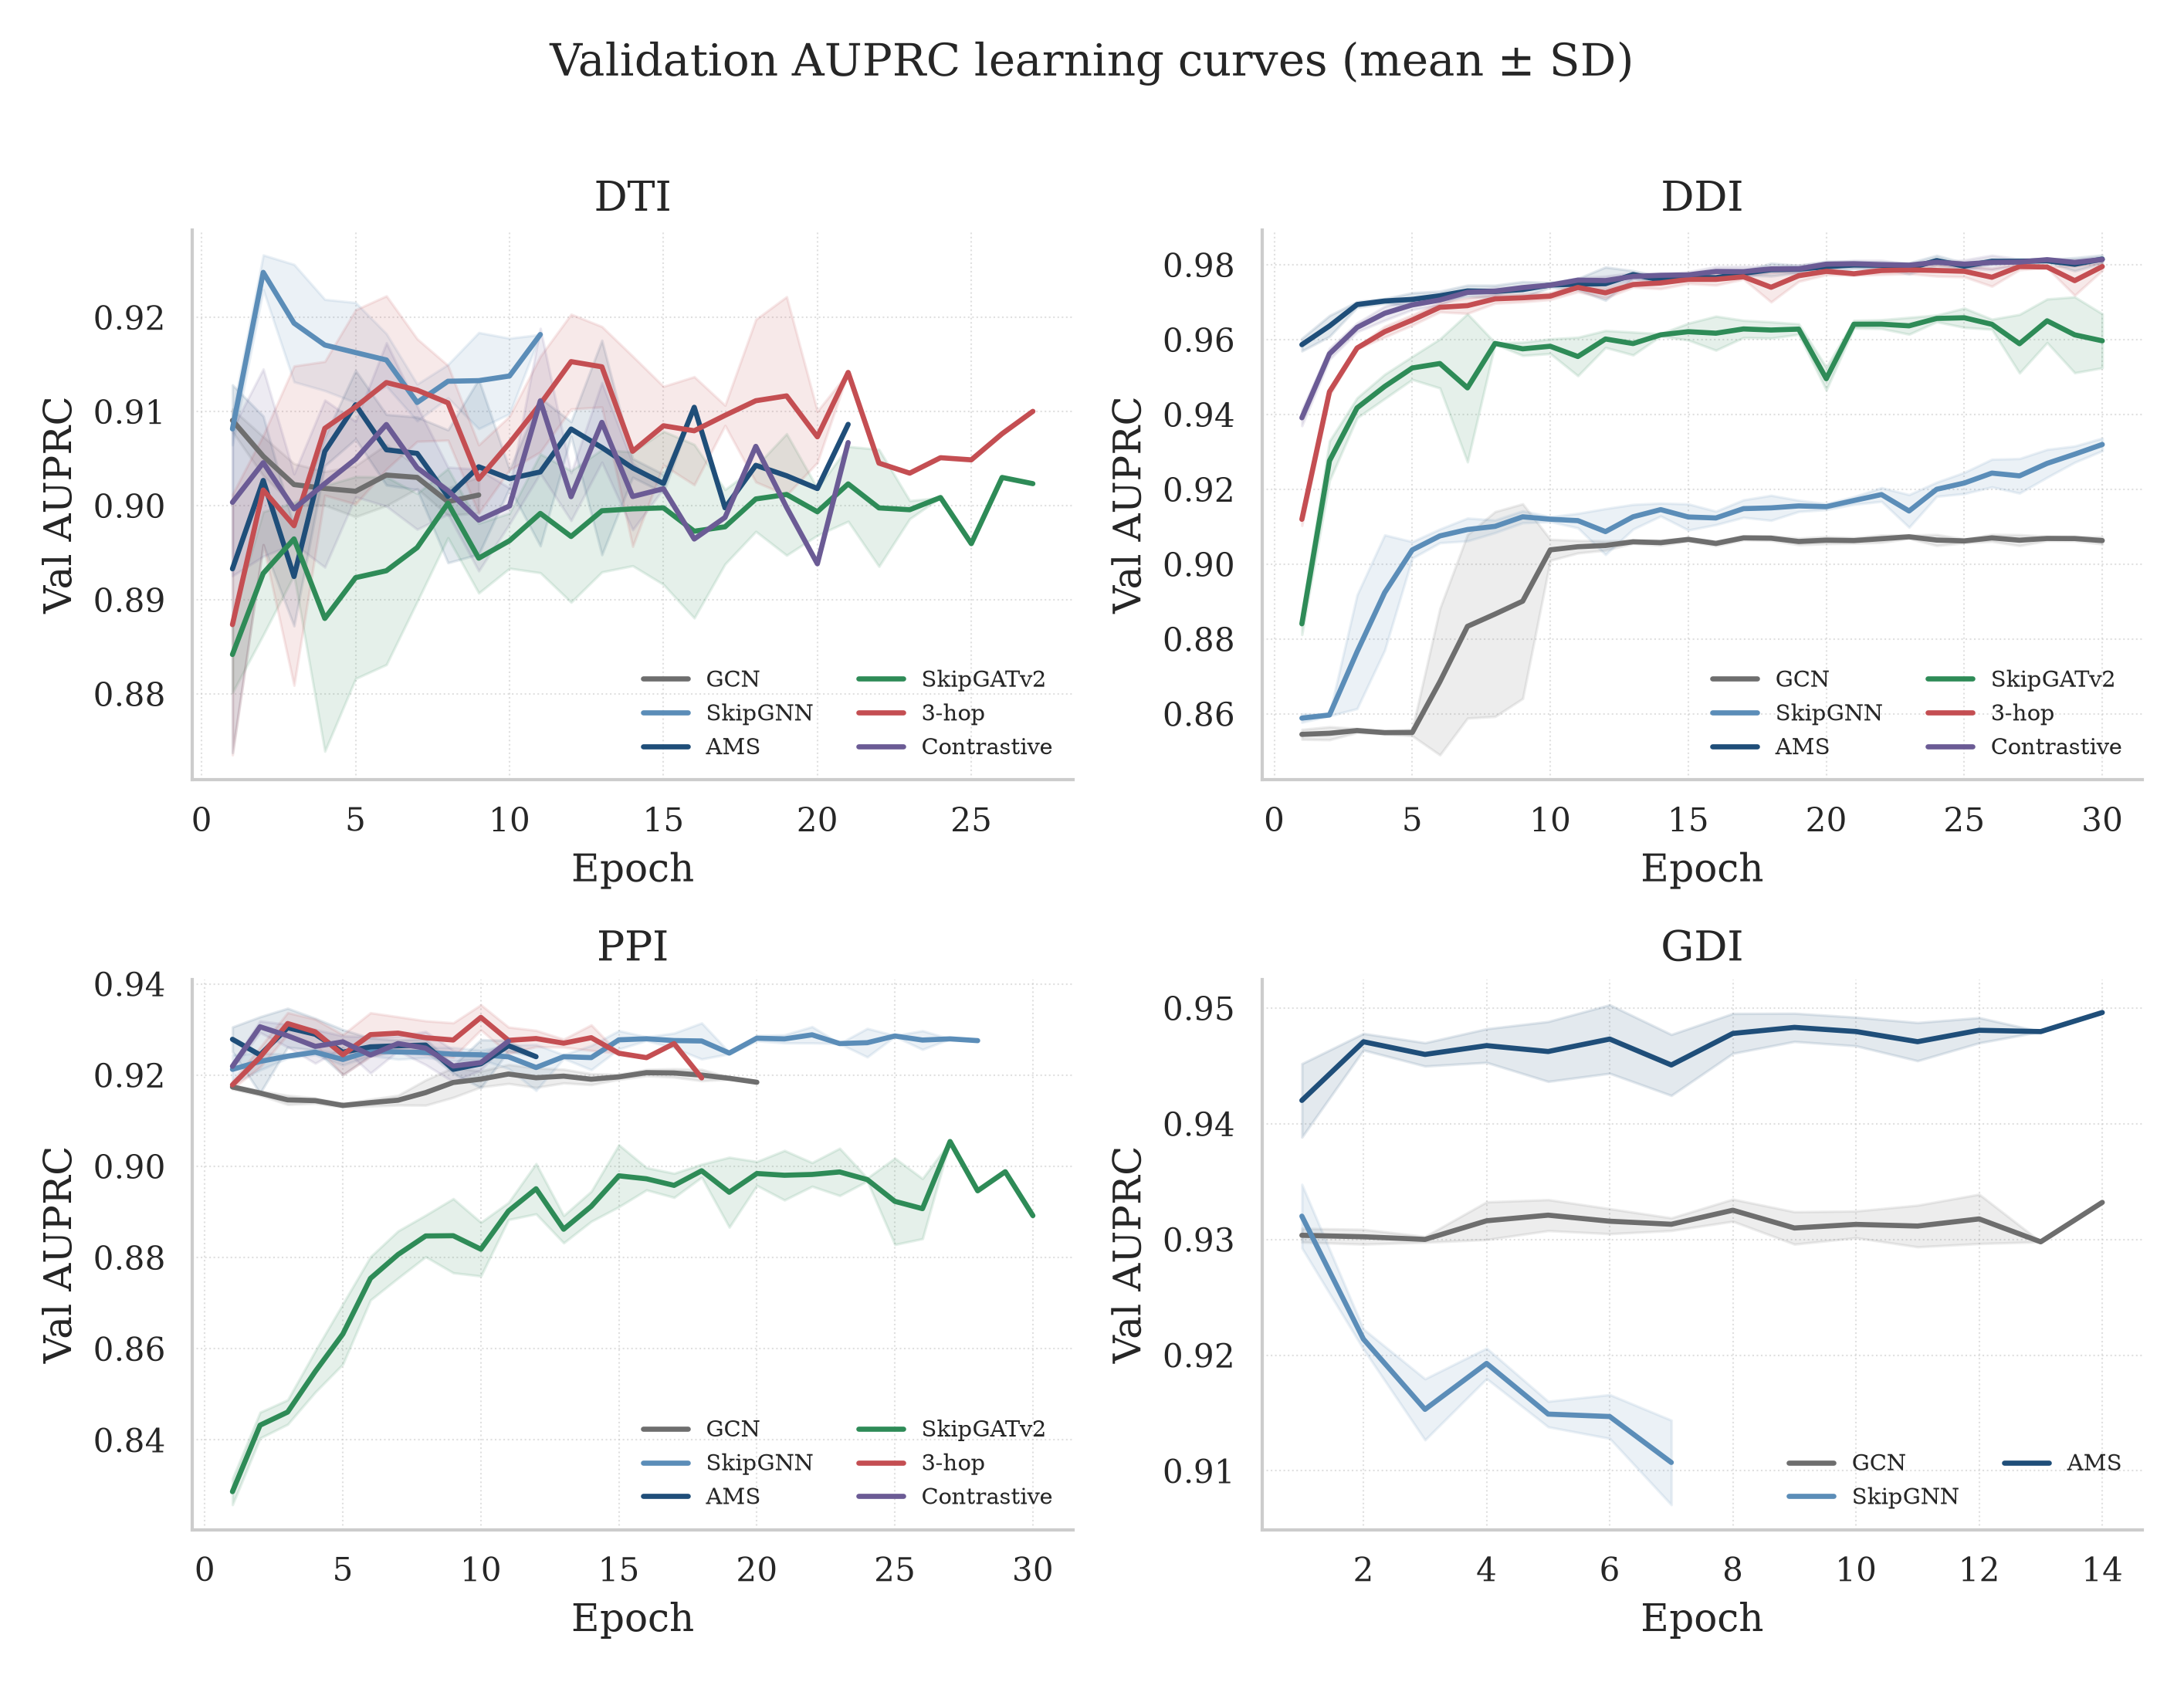
\includegraphics[width=0.98\textwidth]{fig9_learning_curves.png}
\caption[منحنی‌های یادگیری]{منحنی‌های یادگیری: روند \lr{Val AUPRC} در طول اپاک‌های آموزش (میانگین $\pm$ انحراف معیار).}
\label{fig:learning-curves}
\end{figure}


این نمودار چهارپنلی، روند \lr{Val AUPRC} را در طول اپاک‌های آموزش نشان می‌دهد.

\textbf{مشاهدات کلیدی:}

\begin{itemize}
\item \textbf{پنل \lr{DDI}:} مدل‌های پیشنهادی به سرعت به سقف عملکردی ($\approx 0.98$) همگرا می‌شوند. \lr{GCN} در سطح پایین‌تر ($\approx 0.90$) باقی می‌ماند.
\item \textbf{پنل \lr{DTI}:} همگرایی در اپاک‌های اولیه (۳ تا ۸) رخ می‌دهد. مدل \lr{3-hop} روند صعودی ملایم‌تری دارد.
\item \textbf{پنل \lr{PPI}:} \lr{AMS} به سرعت همگرا می‌شود. \lr{SkipGATv2} روند صعودی پیوسته‌تری دارد.
\item \textbf{پنل \lr{GDI}:} پدیده قابل‌توجهی در مدل \lr{SkipGNN} مشاهده می‌شود.
\end{itemize}

\textbf{پدیده افت عملکرد در \lr{SkipGNN} روی \lr{GDI}:}
در پنل \lr{GDI}، مدل مرجع \lr{SkipGNN} از اپاک‌های اولیه با \lr{Val AUPRC} بالا ($\approx 0.93$) شروع شده و سپس روند نزولی تدریجی را طی می‌کند تا جایی که توقف زودهنگام آموزش را متوقف می‌سازد. این الگو با فرضیه بن‌بست هندسی در گراف‌های دوقطبی (بخش ۲-۴-۱) هم‌خوان است: عملگر پرش باینری $\text{\lr{sign}}(A^2)$ در گراف دوقطبی صرفاً اتصالات درون‌نوعی ایجاد می‌کند و با ادامه آموزش، این سیگنال‌های غیرمرتبط به‌تدریج بازنمایی گره‌ها را آلوده می‌سازند.

\textbf{محدودیت تفسیر:} این مشاهده بر اساس ۳ سید است. برای اثبات قطعی این پدیده، تکرار با سیدهای بیشتر و تحلیل آماری رسمی ضروری است.

\subsection{شکل ۱۰: شاخص \lr{F1} در آستانه بهینه}\label{sec:5-3-10}

\begin{figure}[htbp]
\centering
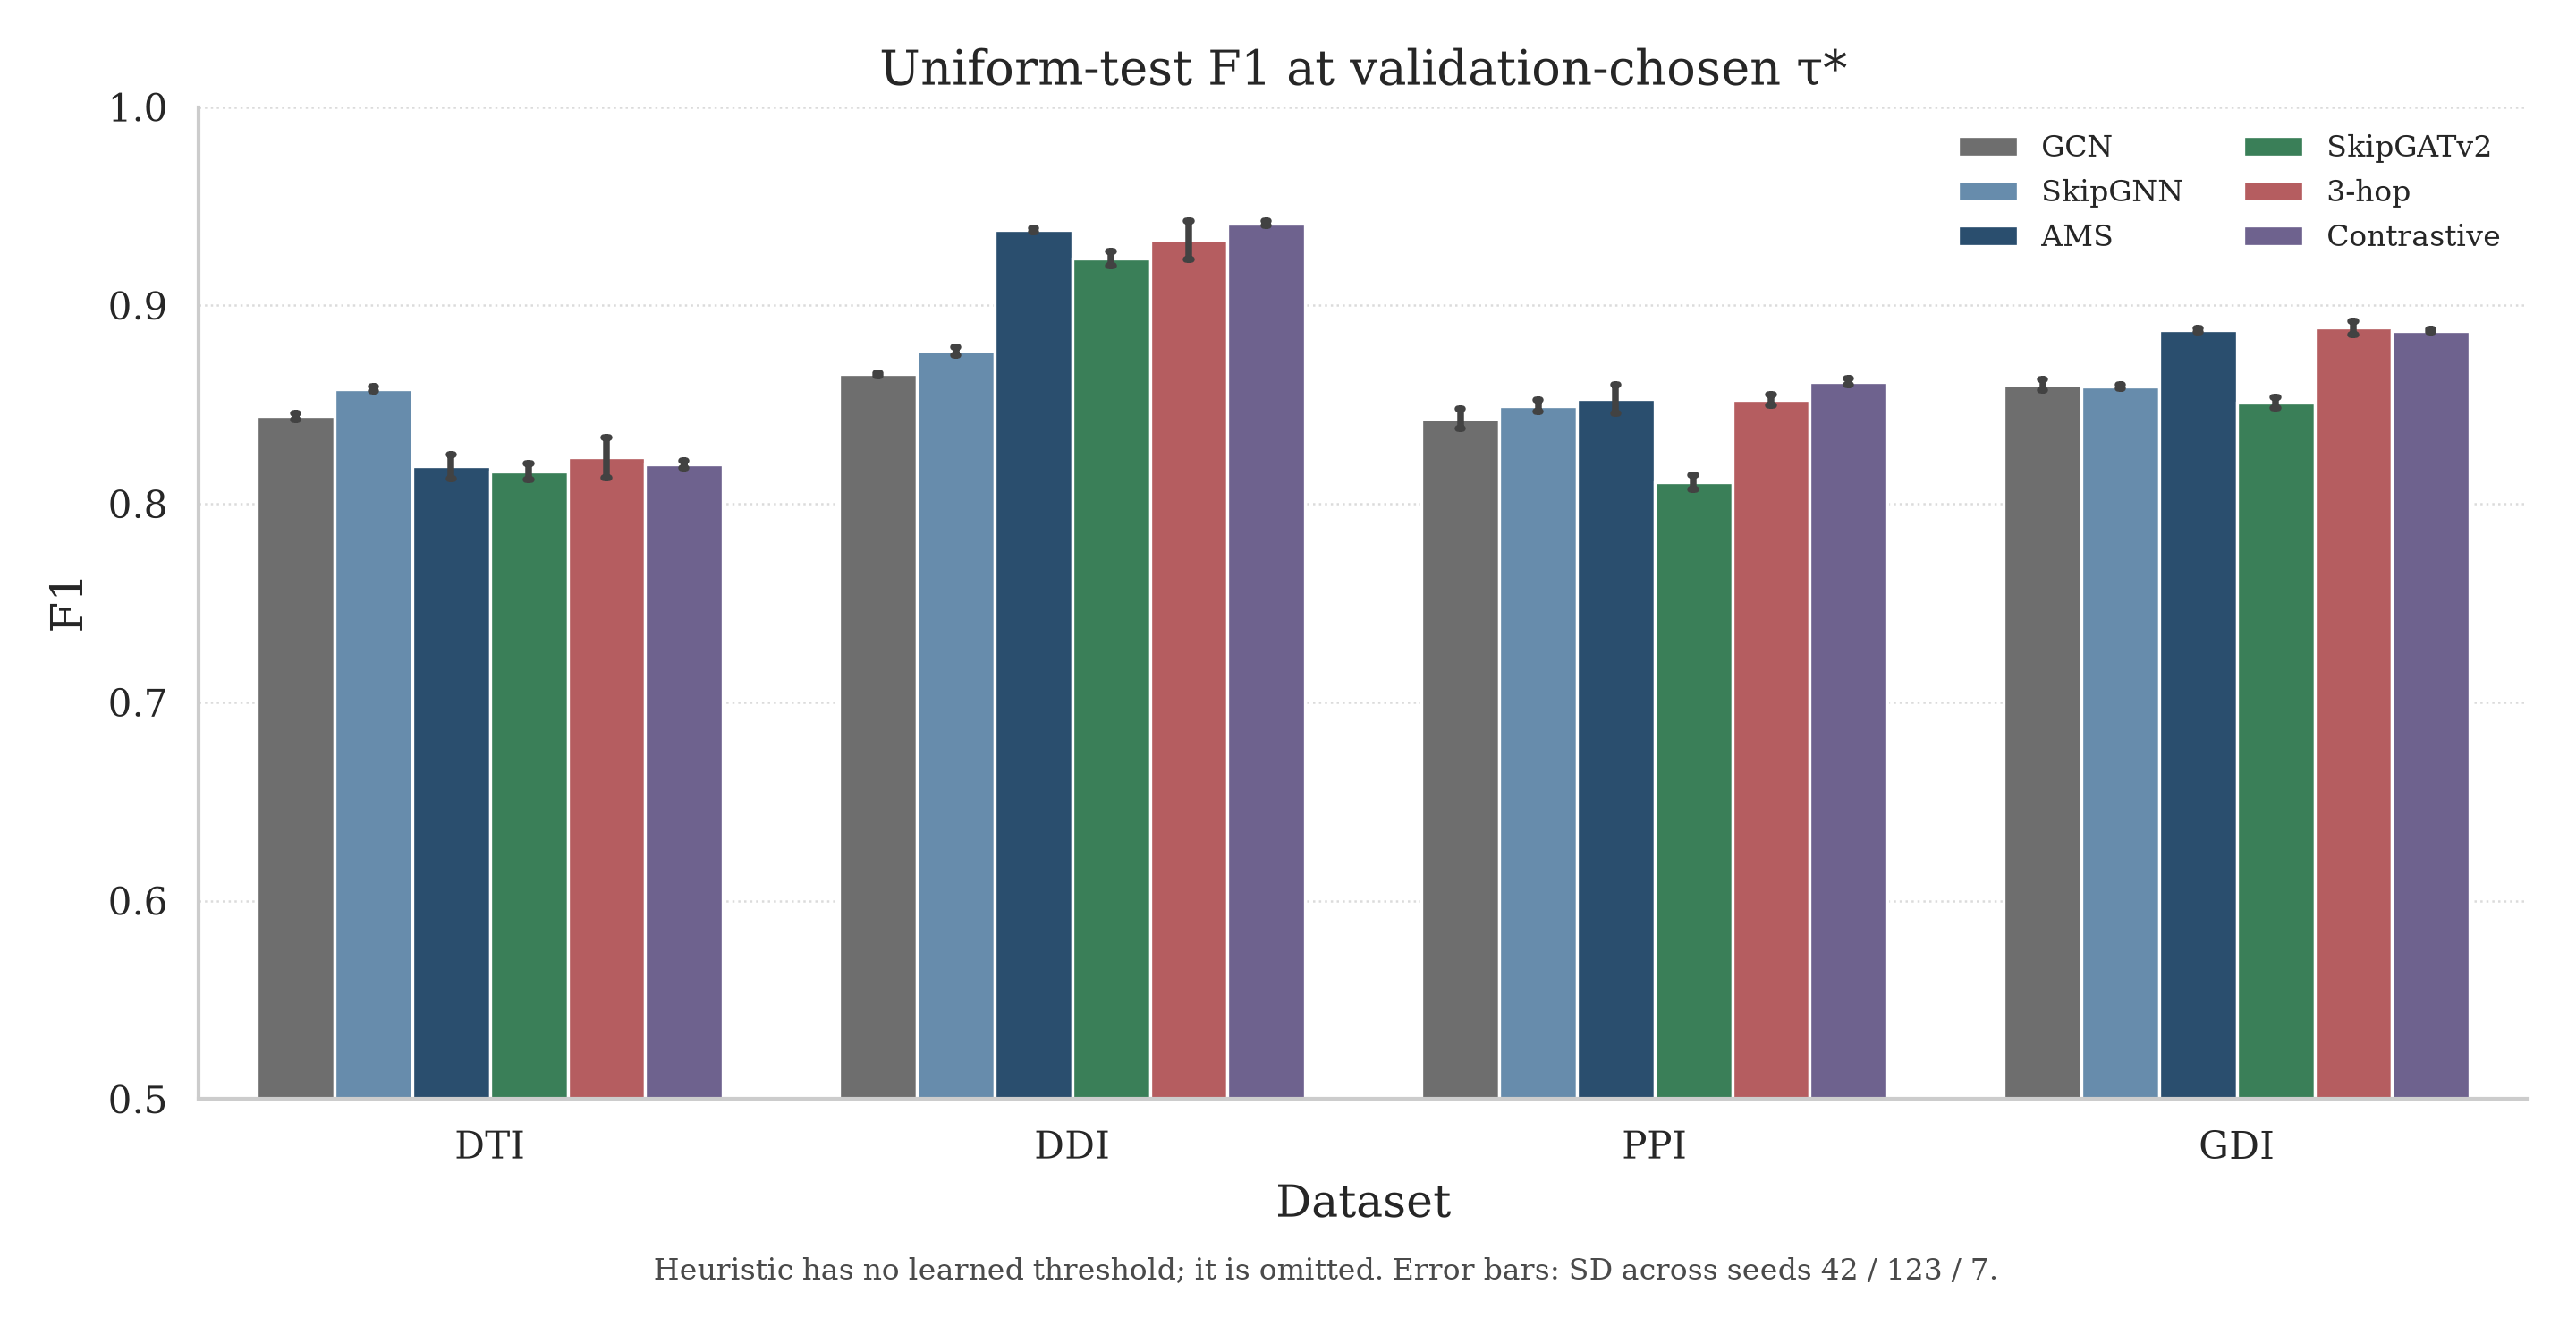
\includegraphics[width=0.98\textwidth]{fig10_f1_at_tau.png}
\caption[شاخص \lr{F1} در آستانۀ بهینه]{شاخص \lr{F1} در آستانۀ منجمد اعتبارسنجی ($\tau^{\ast}$). هوریستیک به‌دلیل نداشتن آستانۀ احتمالی حذف شده است.}
\label{fig:f1-tau}
\end{figure}


این نمودار شاخص \lr{F1} را در آستانه منجمد اعتبارسنجی ($\tau^*$) گزارش می‌کند. هوریستیک به دلیل فاقد بودن آستانه احتمالی حذف شده است.

\textbf{مشاهدات:}
\begin{itemize}
\item در \lr{DDI}، شاخص \lr{F1} برای \lr{AMS}، \lr{Contrastive} و \lr{3-hop} به بالای $0.93$ می‌رسد.
\item در \lr{GDI}، مدل‌های \lr{3-hop} و \lr{Contrastive} با \lr{F1} حدود $0.889$ بالاترین تعادل را نشان می‌دهند.
\item در \lr{PPI}، \lr{SkipGATv2} با \lr{F1} حدود $0.809$ بالاترین تعادل را دارد.
\end{itemize}

\section{تحلیل فضاهای نهفته با \lr{t-SNE}}\label{sec:5-4}


\begin{figure}[htbp]
\centering
\begin{minipage}{0.48\textwidth}\centering
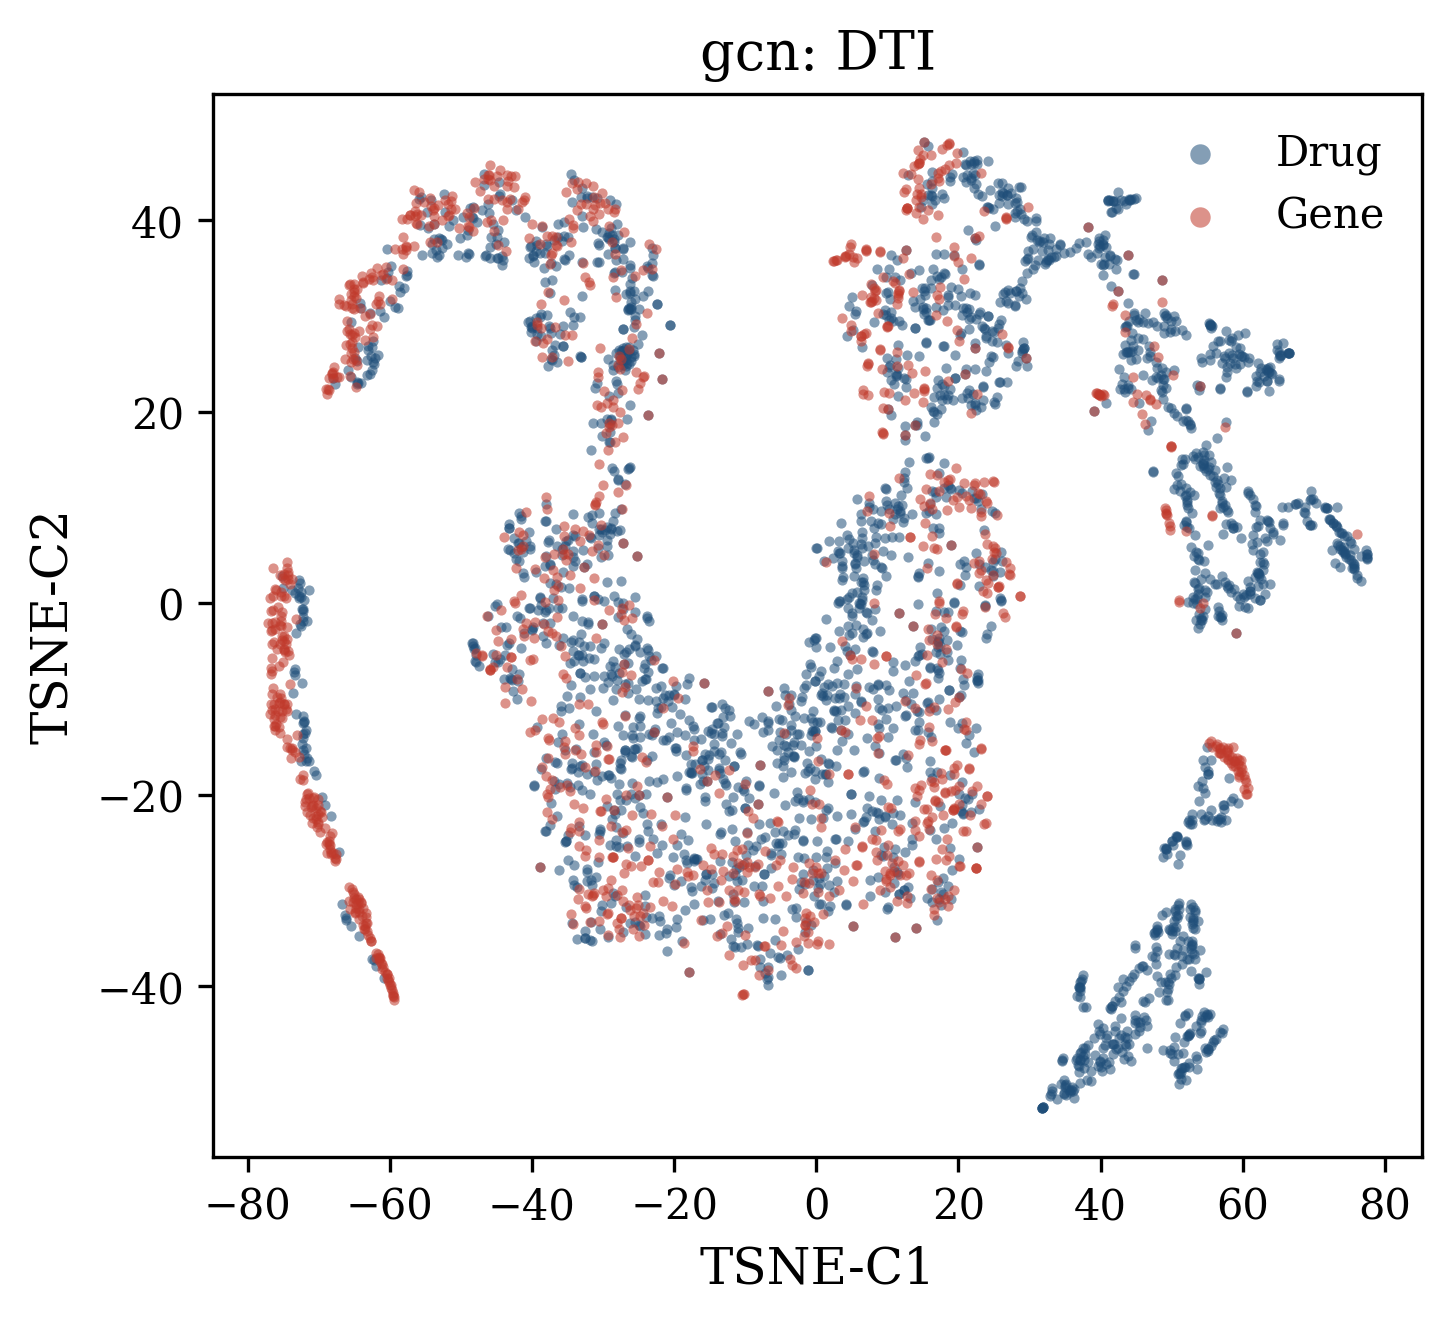
\includegraphics[width=\linewidth]{fig_tsne_DTI_gcn_seed42.png}\\[2pt]
{\small \lr{GCN}}
\end{minipage}\hfill
\begin{minipage}{0.48\textwidth}\centering
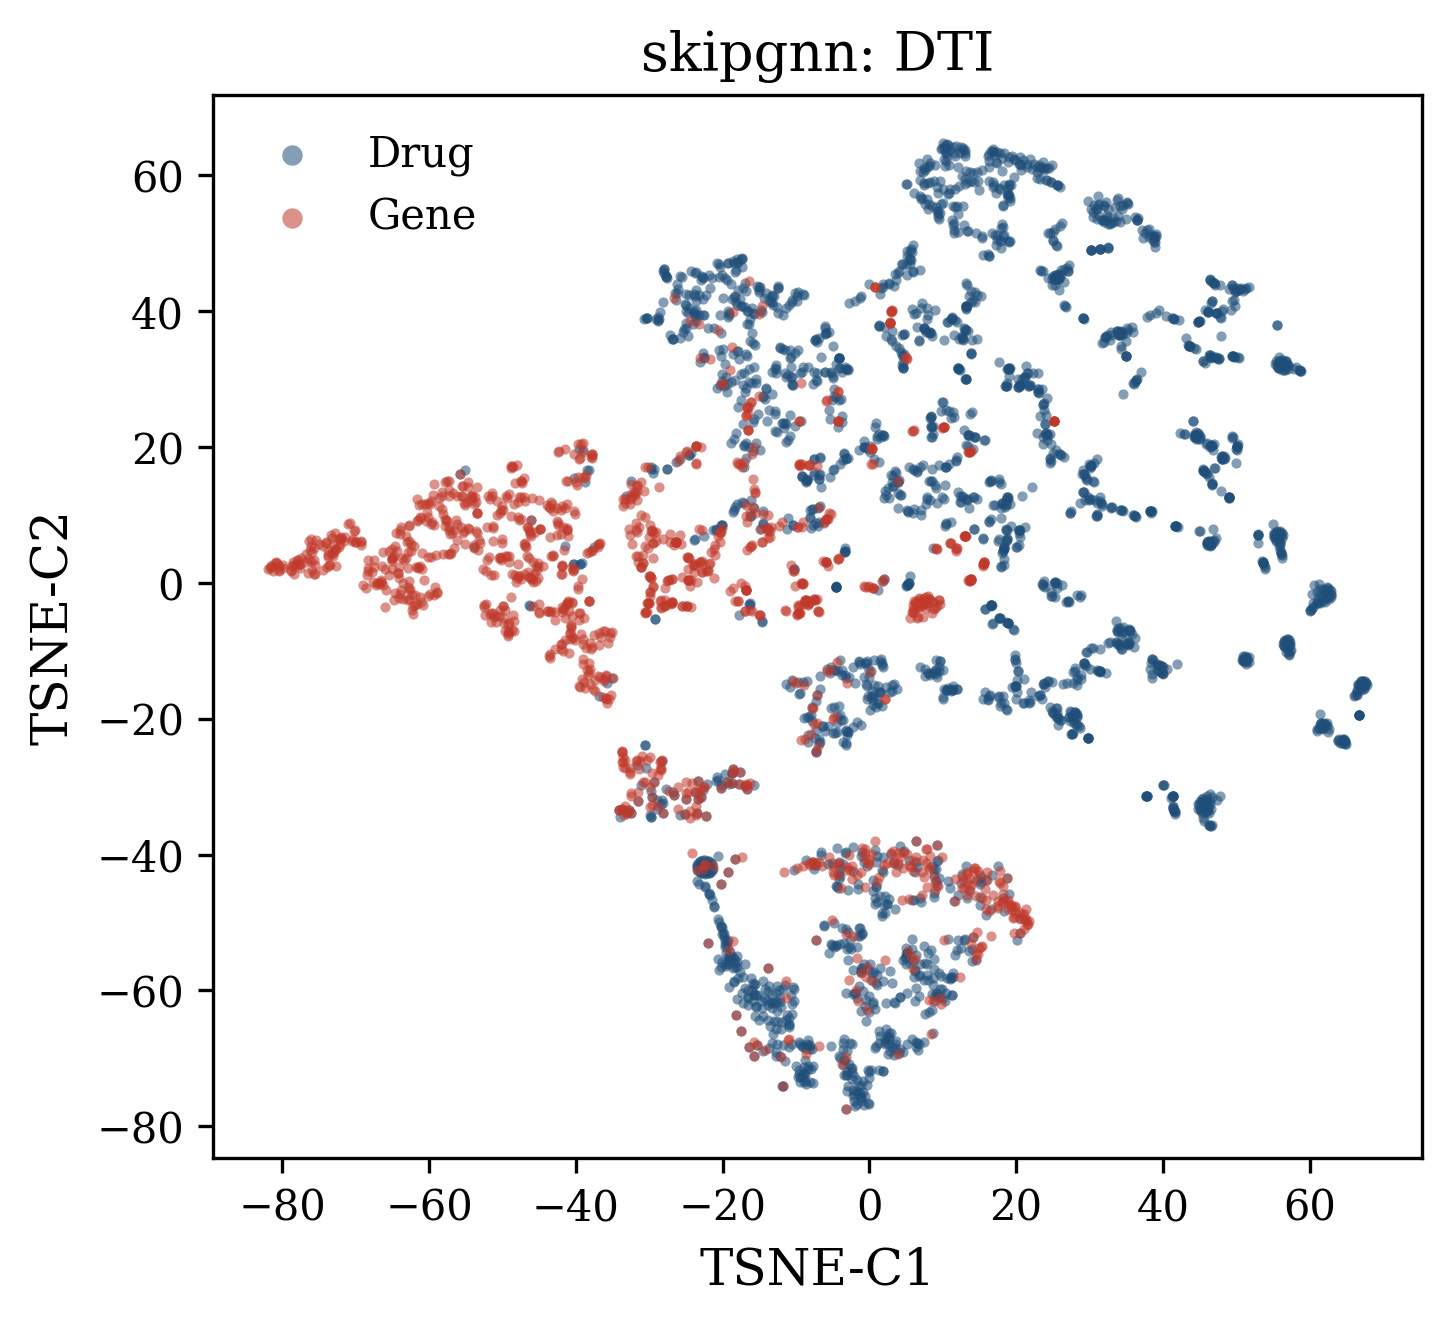
\includegraphics[width=\linewidth]{fig_tsne_DTI_skipgnn_seed42.png}\\[2pt]
{\small \lr{SkipGNN}}
\end{minipage}\\[8pt]
\begin{minipage}{0.48\textwidth}\centering
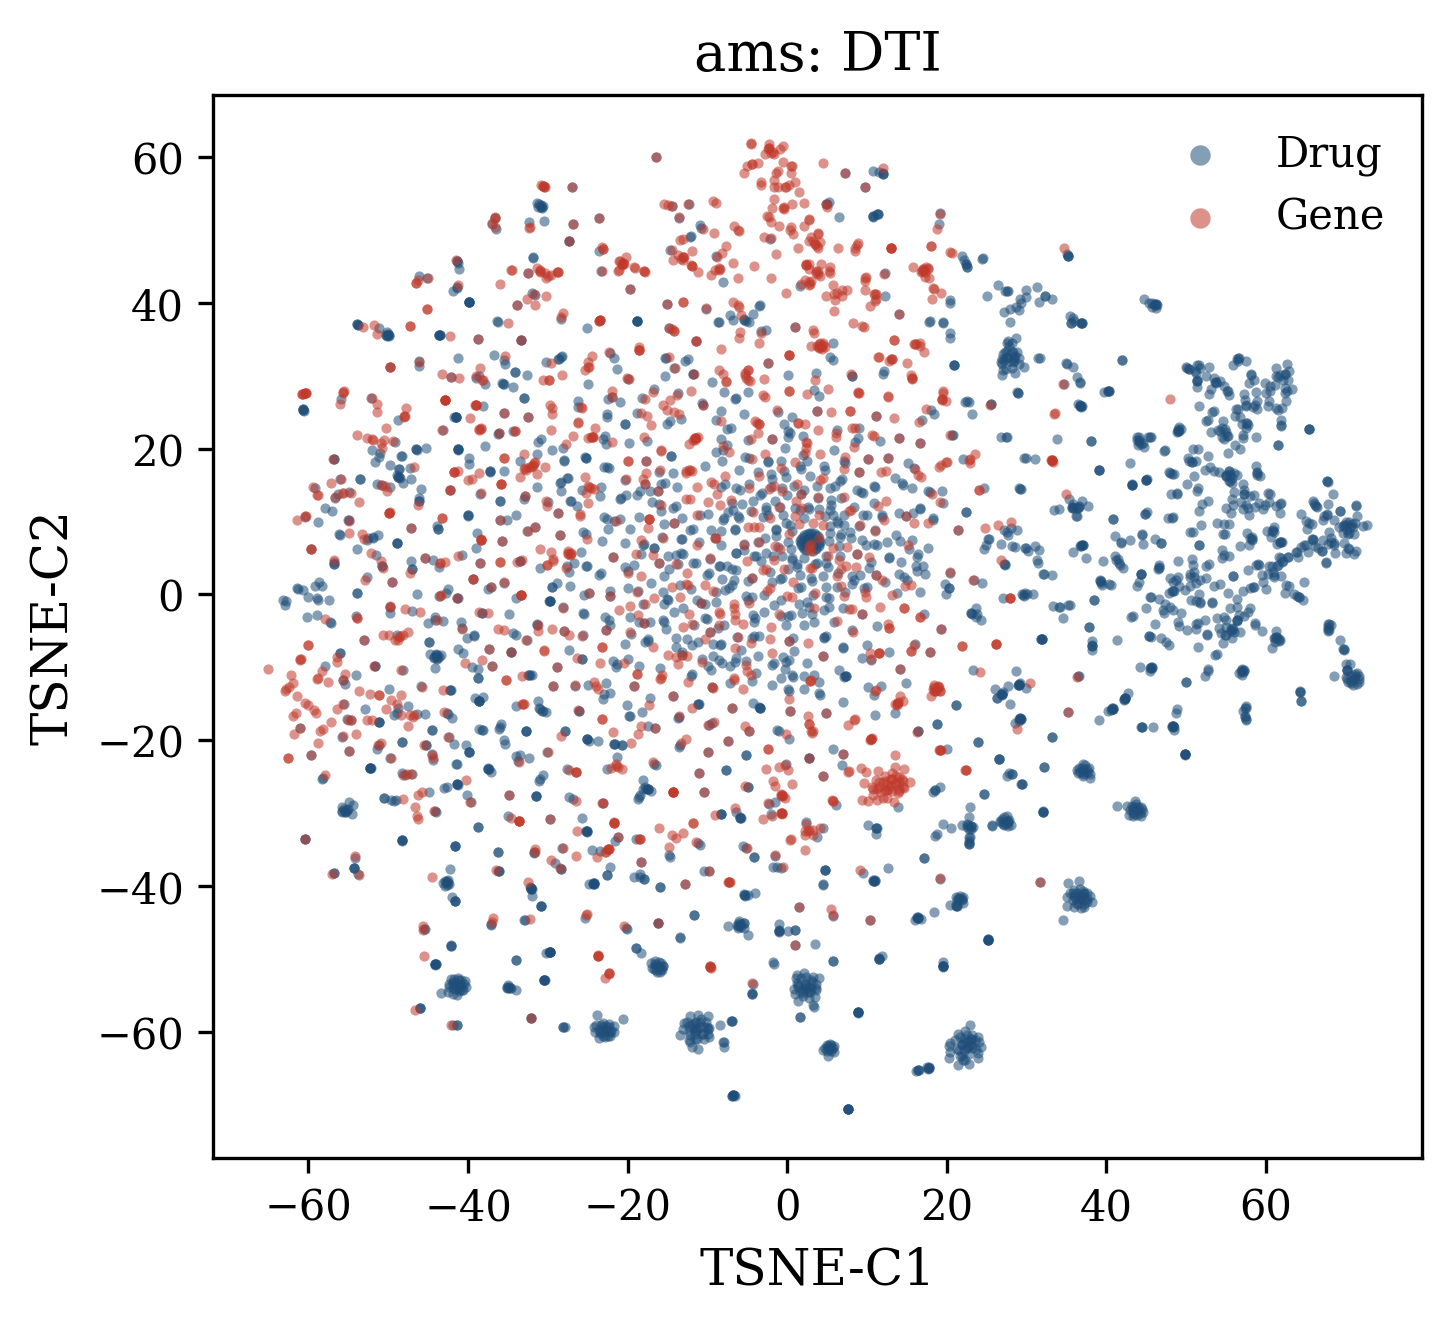
\includegraphics[width=\linewidth]{fig_tsne_DTI_ams_seed42.png}\\[2pt]
{\small \lr{AMS-SkipGNN}}
\end{minipage}\hfill
\begin{minipage}{0.48\textwidth}\centering
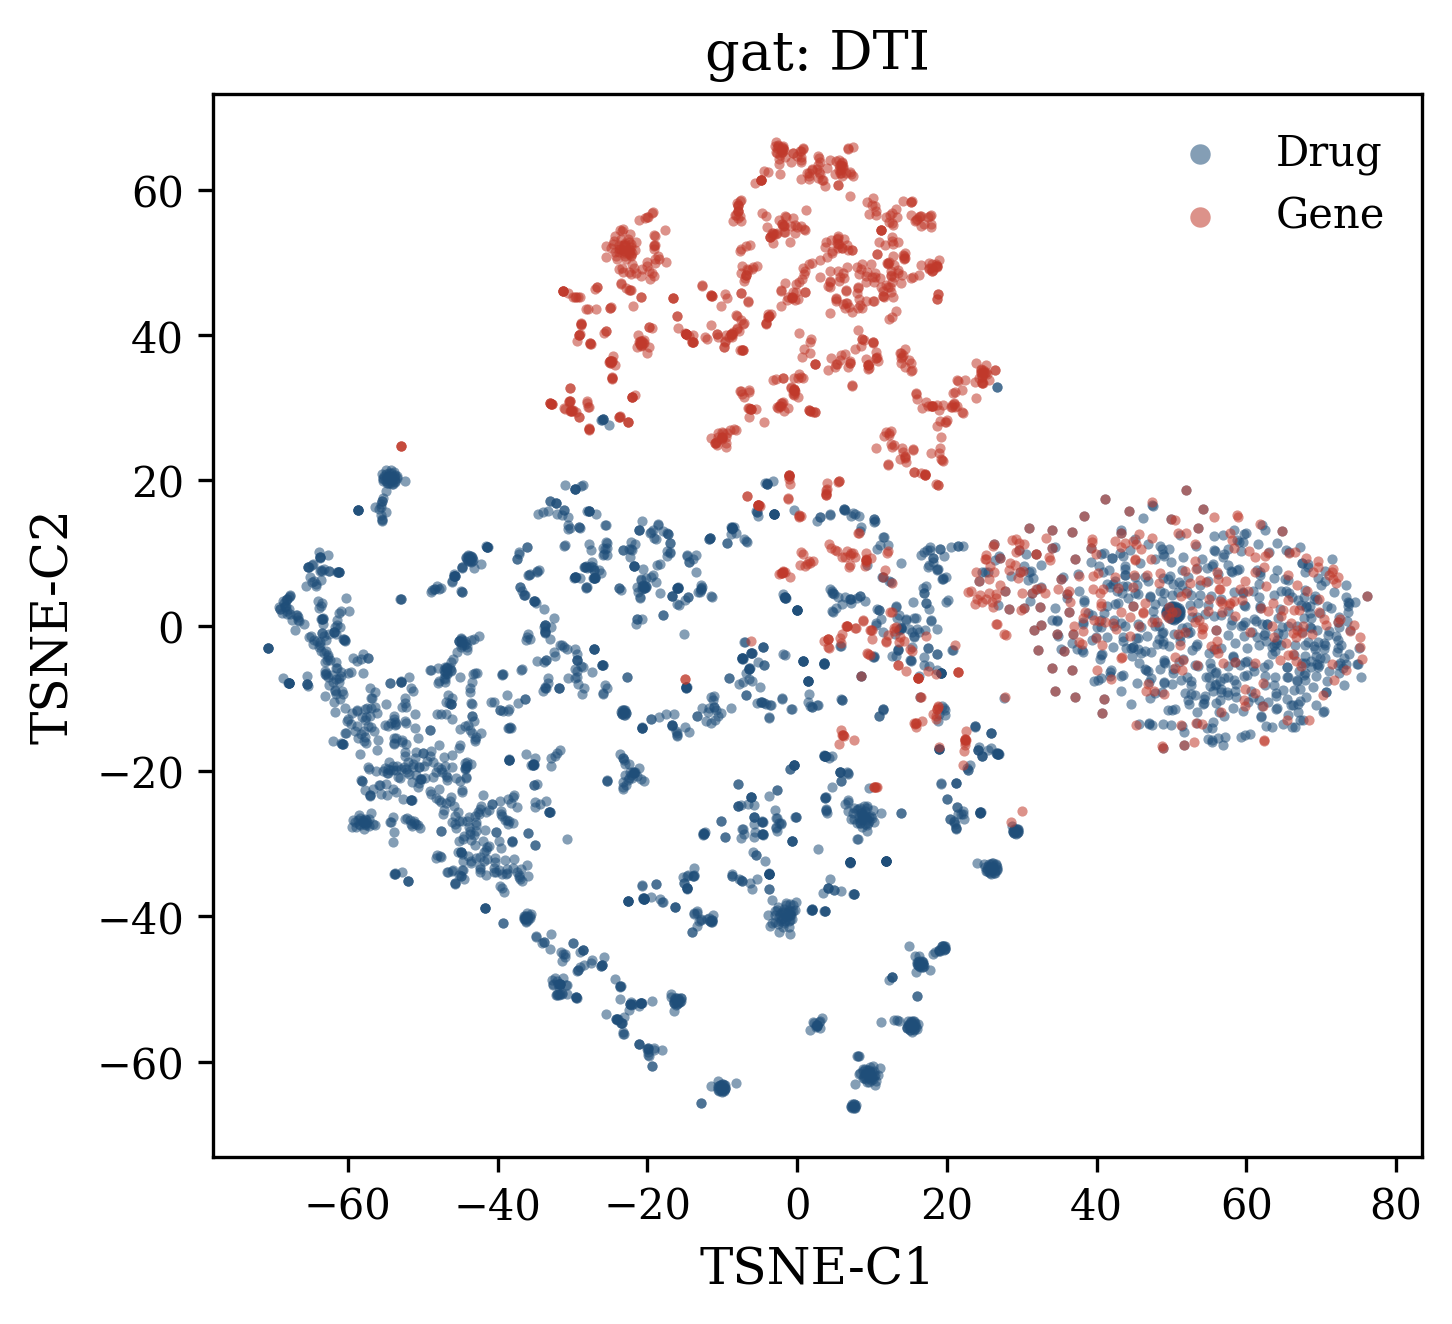
\includegraphics[width=\linewidth]{fig_tsne_DTI_gat_seed42.png}\\[2pt]
{\small \lr{SkipGATv2}}
\end{minipage}
\caption[تصویرسازی \lr{t-SNE} لایۀ آخر]{تصویرسازی \lr{t-SNE} از امبدینگ لایۀ آخر روی دیتاست \lr{DTI} (سید ۴۲). رنگ‌ها نوع موجودیت را در گراف دوقطبی نشان می‌دهند.}
\label{fig:tsne-dti}
\end{figure}


برای درک شهودی از چگونگی سازمان‌دهی فضا توسط انکودرها، امبدینگ‌های لایه آخر مدل‌ها در سید ۴۲ توسط الگوریتم \lr{t-SNE} \cite{maaten2008tsne} تصویرسازی شدند. پارامترهای تصویرسازی:
\begin{itemize}
\item کاهش بعد از ۶۴ به ۲
\item نمونه‌برداری حداکثر ۴۰۰۰ گره
\item رنگ‌آمیزی بر اساس نوع موجودیت (مبدا/مقصد) در گراف‌های دوقطبی
\item \pcode{perplexity = min(30, max(5, N/10))}
\item \pcode{init = "pca"}
\end{itemize}


\begin{table}[htbp]
\centering
\footnotesize
\caption{تحلیل تطبیقی ویژگی‌های بصری مانیفولد فضای نهفته}
\label{tab:5-6}
\begin{tabular}{llll}
\toprule
مدل & ساختار هندسی مشاهده‌شده & تفکیک نوع موجودیت & تفسیر \\
\midrule
\lr{GCN} & رشته‌ای و درهم‌تنیده & تفکیک ضعیف & محو هویت ساختاری گره‌ها \\
\lr{SkipGNN} & دو قطب مجزا با مرز خشک & تفکیک ماکروسکوپیک & تراکم ناشی از باینری‌سازی \\
\lr{AMS} & مدولار با هسته و حاشیه & تفکیک پیوسته & وزن‌دهی پیوسته و حفظ تنوع \\
\lr{3-hop} & پل‌های ارتباطی میان خوشه‌ها & تفکیک با اتصالات مرزی & اتصال خانواده‌های ساختاری \\
\lr{Contrastive} & توزیع یکنواخت & توزیع متعادل & اثر زیان مقابله‌ای \\
\lr{SkipGATv2} & جزایر خوشه‌ای مجزا & خوشه‌بندی تمیز & هرس یال‌های کم‌اهمیت \\
\bottomrule
\end{tabular}
\end{table}


\textbf{ملاحظات روش‌شناختی:} تحلیل \lr{t-SNE} توصیفی و کیفی است. برای ارزیابی کمّی کیفیت فضای نهفته، معیارهایی مانند \lr{Silhouette Score}، \lr{Alignment} و \lr{Uniformity} \cite{wang2020uniformity}، یا دقت طبقه‌بندی \lr{k-NN} روی فضای نهفته می‌توانند مکمل مفیدی باشند. این معیارها به‌عنوان کار آینده پیشنهاد می‌شوند.

\section{خلاصه یافته‌های کلیدی فصل}\label{sec:5-5}


جدول ۵-۷ خلاصه‌ای از بهبودهای کلیدی مدل‌های پیشنهادی نسبت به مدل مرجع \lr{SkipGNN} را در معیار اصلی رتبه‌بندی (\lr{Hard AUPRC}) نشان می‌دهد. مقادیر بهبود به واحد درصد (\lr{percentage points}) بیان شده‌اند:


\begin{table}[htbp]
\centering
\footnotesize
\caption{بهبود مطلق نسبت به \lr{SkipGNN} در \lr{Hard AUPRC}}
\label{tab:5-7}
\begin{tabular}{lllll}
\toprule
دیتاست & \lr{SkipGNN} & بهترین مدل پیشنهادی & بهبود مطلق (واحد درصد) & وضعیت آماری \\
\midrule
\lr{DDI} & $0.724$ & \lr{AMS}: $0.912$ & $+0.188$ & برتری بدون هم‌پوشانی بازه‌ها \\
\lr{PPI} & $0.622$ & \lr{SkipGATv2}: $0.778$ & $+0.156$ & برتری بدون هم‌پوشانی بازه‌ها \\
\lr{GDI} & $0.720$ & \lr{SkipGATv2}: $0.837$ & $+0.117$ & برتری مرزی \\
\lr{DTI} & $0.695$ & \lr{AMS}، \lr{SkipGATv2} و \lr{3-hop} هم‌سطح & $+0.10$ تا $+0.11$ & هم‌سطح آماری (بازه‌های هم‌پوشان) \\
\bottomrule
\end{tabular}
\end{table}


\textbf{یافته‌های مکمل:}
\begin{itemize}
\item در دیتاست \lr{PPI}، \lr{SkipGATv2} با اختلاف $+0.104$ واحد درصد از \lr{AMS} پیشی گرفته است. این برتری با وجود گام‌های بهینه‌سازی کمتر (۳۱ در برابر ۲۵۵ گام در هر اپاک) رخ داده است.
\item در دیتاست \lr{GDI}، هوریستیک تحلیلی با $0.842$ بالاتر از تمام مدل‌های عصبی است.
\item در دیتاست \lr{DDI}، \lr{AMS} با $0.912$ برترین عملکرد را در میان مدل‌های عصبی دارد.
\end{itemize}


\chapter{بحث، تحلیل پاشنه‌های آشیل، نتیجه‌گیری و افق‌های آینده}
% Auto-generated from report/6.md — do not edit by hand.
\section{بحث مکانیکی و تبیین چرایی نتایج (\lr{Mechanistic Discussion})}\label{sec:6-1}


یافته‌های تجربی ارائه‌شده در فصل پنجم، پنج فرضیه علمی مطرح‌شده در فصل اول را تا حد زیادی تایید می‌کنند. واکاوی رفتار مدل‌ها در چهار بنچمارک زیستی، سه بینش بنیادین تئوریک پیرامون دینامیک یادگیری روی گراف‌های زیست‌مولکولی را آشکار می‌سازد.

\subsection{نقش عملگر پیوسته تخصیص منابع در مهار سوگیری هاب‌ها}\label{sec:6-1-1}


یکی از مهم‌ترین یافته‌های این پژوهش، تاثیر جایگزینی عملگر باینری $\text{\lr{sign}}(AA^T)$ با عملگر پیوسته تخصیص منابع ($W_2 = AD^{-1}A^T$) است. در گراف‌های زیستی که دارای توزیع درجه بی‌مقیاس هستند، گره‌های هاب (مانند داروهای پرعارضه یا پروتئین‌های چندمنظوره) به‌طور مصنوعی تعداد زیادی مسیر ۲-گام ایجاد می‌کنند.

عملگر باینری \lr{SkipGNN}، تمام این مسیرها را با وزن یکسان ($1.0$) لحاظ می‌کند که منجر به پدیده «اشباع سیگنال» در گره‌های هاب می‌شود. در مقابل، عملگر تخصیص منابع با تقسیم وزن هر مسیر بر درجه گره واسط ($1/d_k$)، به‌عنوان یک فیلتر پایین‌گذر توپولوژیک عمل کرده و سیگنال‌های اختصاصی (از طریق گره‌های واسط با درجه پایین) را تقویت می‌کند. این مکانیزم دلیل اصلی جهش عملکرد مدل \lr{AMS} در دیتاست متراکم \lr{DDI} (از $0.724$ به $0.912$ در آزمون سخت، معادل بهبود $+0.188$ واحد درصد) است، جایی که تداخلات دارویی از طریق مسیرهای چندگانه و پیچیده شکل می‌گیرند.

\subsection{حل بن‌بست هندسی دوقطبی با مسیرهای ۳-گام}\label{sec:6-1-2}


همان‌طور که در بخش ۲-۴-۱ اثبات شد، در گراف‌های دوقطبی (\lr{DTI} و \lr{GDI})، ماتریس $A^2$ ساختاری بلوکی-قطری دارد و فاقد هرگونه یال میان موجودیت‌های ناهم‌نوع است. مدل مرجع \lr{SkipGNN} با تکیه بر این ماتریس، در عمل دچار افت عملکرد تدریجی می‌شد (مشاهده‌شده در منحنی‌های یادگیری \lr{GDI} در شکل ۹).

مدل‌های \pcode{ThreeHopSkipGNN} و \pcode{AMS-SkipGNN} با تزریق صریح مسیرهای ۳-گام ($W_3 = W_2 D^{-1} A$)، این بن‌بست هندسی را شکستند. مسیر $d \to p' \to d' \to p$ (دارو \faarrow{} پروتئین واسط \faarrow{} داروی واسط \faarrow{} پروتئین هدف) اولین مسیر توپولوژیک غیرمستقیم برای دسترسی به تارگت کاندید است. موفقیت این مدل‌ها در دیتاست \lr{DTI} (کسب \lr{Hard AUPRC} برابر با $0.803$ برای \lr{3-hop} و $0.798$ برای \lr{AMS}) نشان می‌دهد که دسترسی انکودر به اطلاعات نوع مخالف، پیش‌شرط یادگیری در گراف‌های دوقطبی است.

\subsection{هم‌افزایی گیتینگ تطبیقی و دیکودر تانسوری تعاملی}\label{sec:6-1-3}


تحلیل نردبان ابلیشن (شکل ۲) یک الگوی قابل‌توجه را نشان داد: افزودن پرش وزن‌دار (گام ۱) و گیتینگ تطبیقی (گام ۲) به‌تنهایی و بدون اصلاح دیکودر، نه‌تنها بهبودی ایجاد نکرد، بلکه منجر به افت جزئی عملکرد (از $0.703$ به $0.686$ در \lr{DTI}) شد.

\textbf{تبیین مکانیکی:} پرش پیوسته \lr{RA} و گیتینگ، ظرفیت بازنمایی (\lr{Representation Capacity}) شبکه را به‌شدت افزایش می‌دهند و سیگنال‌های توپولوژیک غنی‌تری تولید می‌کنند. با این حال، دیکودر خطی الحاقی ($[E_u \parallel E_v]$) فاقد ظرفیت لازم برای پردازش این سیگنال‌های پیچیده و غیرخطی است. در نتیجه، شبکه دچار بیش‌برازش روی نویزهای فرکانس‌بالای گراف پرش می‌شود.

جهش اصلی در گام ۳ (افزودن دیکودر تانسوری ۴‌گانه) رخ داد. مولفه‌های ضربی ($E_u \odot E_v$) و فاصله‌ای ($|E_u - E_v|$) در این دیکودر، تقارن ذاتی تعاملات بیوشیمیایی (مانند مدل قفل‌وکلید) را به‌صورت صریح مدل‌سازی می‌کنند. این یافته نشان می‌دهد که در معماری‌های \lr{GNN}، ارتقای انکودر باید همواره با ارتقای متناسب ظرفیت دیکودر همراه باشد تا از پدیده «تنگنای اطلاعاتی» (\lr{Information Bottleneck}) جلوگیری شود.

\subsection{تمایز عملکرد بین دیتاست‌ها و کارآمدی \lr{SkipGATv2}}\label{sec:6-1-4}


یکی از یافته‌های مهم این پژوهش، تفاوت الگوی برتری مدل‌ها در دیتاست‌های مختلف است:

\begin{itemize}
\item \textbf{\lr{DDI} (گراف همگن متراکم):} مدل \lr{AMS} با $0.912$ برترین عملکرد را دارد، و برتری آن نسبت به سایر مدل‌های پیشنهادی کاملاً آشکار است.
\item \textbf{\lr{DTI} (گراف دوقطبی تنک):} سه مدل \lr{AMS}، \lr{SkipGATv2} و \lr{3-hop} با میانگین‌های $0.798$، $0.804$ و $0.803$ از نظر آماری هم‌سطح هستند (بازه‌های انحراف معیار هم‌پوشان).
\item \textbf{\lr{PPI} (گراف همگن مدولار):} \lr{SkipGATv2} با $0.778$ بهترین عملکرد را دارد که بهبود قابل‌توجه $+0.104$ واحد درصدی نسبت به \lr{AMS} نشان می‌دهد.
\item \textbf{\lr{GDI} (گراف دوقطبی کلان):} هوریستیک تحلیلی با $0.842$ بالاتر از تمام مدل‌های عصبی است.
\end{itemize}

\textbf{تحلیل \lr{SkipGATv2} در \lr{PPI}:} نکته مهم این است که برتری \lr{SkipGATv2} در \lr{PPI} \textbf{علی‌رغم} گام‌های بهینه‌سازی کمتر رخ داده است. این مدل در \lr{PPI} تنها ۳۱ گام \lr{Adam} در هر اپاک دریافت کرده (در مقایسه با ۲۵۵ گام \lr{AMS}، به دلیل بچ‌سایز ۱۰۲۴ در برابر ۱۲۸). این برتری با وجود گام‌های بهینه‌سازی کمتر، به‌عنوان شواهدی بر کارآمدی ذاتی مکانیزم توجه پویا در گراف‌های همگن مدولار تفسیر می‌شود، نه صرفاً نتیجه بودجه محاسباتی بیشتر.

\section{تحلیل پاشنه‌های آشیل و محدودیت‌های روش‌شناختی}\label{sec:6-2}


یک گزارش علمی معتبر موظف است محدودیت‌ها و شرایط مرزی مدل‌های خود را به‌صورت شفاف و بدون اغراق تبیین کند. تحلیل نتایج، چهار چالش و محدودیت مهم را آشکار می‌سازد که مسیرهای اصلی برای کارهای آینده هستند.

\subsection{چالش گراف‌های کلان و تنک: برتری هوریستیک در \lr{GDI}}\label{sec:6-2-1}


یکی از مهم‌ترین و صادقانه‌ترین یافته‌های این پژوهش، عملکرد خیره‌کننده هوریستیک تحلیلی \lr{Resource Allocation} در دیتاست ژن-بیماری (\lr{GDI}) است. در این گراف دوقطبی کلان ($19{,}783$ نود)، هوریستیک ۳-گام بدون هیچ پارامتر یادگیرنده‌ای، \lr{Hard AUPRC} برابر با $0.842$ کسب کرد که بالاتر از تمام مدل‌های عصبی (از جمله \lr{SkipGATv2} با $0.837$ و \lr{AMS} با $0.829$) است.

\textbf{تحلیل ریشه‌ای:} این پدیده که در ادبیات \lr{GNN}ها به عنوان «محدودیت سوگیری القایی» (\lr{Inductive Bias Limitation}) شناخته می‌شود، نشان می‌دهد که در گراف‌های به‌شدت تنک و کلان با ویژگی‌های هویتی، مکانیزم \lr{Message-Passing} در \lr{GNN}ها (حتی با وجود پرش‌های وزنی و گیتینگ) دچار پدیده «رقیق‌شدن سیگنال» (\lr{Signal Dilution}) می‌شود. هوریستیک \lr{RA} ذاتاً یک شمارشگر دقیق و بهینه مسیرهای ۳-گام است و در غیاب ویژگی‌های غنیِ گره‌ای (\lr{Node Features})، توپولوژی خالص را بهتر از یک شبکه عصبی ۲-لایه استخراج می‌کند.

\textbf{تبیین صادقانه:} این یافته نشان می‌دهد که معماری‌های عصبی برای غلبه بر هوریستیک‌ها در گراف‌های کلان، نیازمند تلفیق با ویژگی‌های معنادار بیوشیمیایی هستند تا صرفاً توپولوژی. به بیان دیگر، در این پژوهش با انتخاب آگاهانه ویژگی‌های هویتی (بخش ۱-۵-۲)، ما به‌طور عمدی مزیت ویژگی‌های بیوشیمیایی را حذف کردیم تا اثر خالص معماری را بسنجیم. این محدودیت به‌صراحت به‌عنوان مسیر کار آینده ذکر شده است.

\subsection{محدودیت ویژگی‌های هویتی (\lr{One-Hot}) و افت مکانیزم توجه در گراف کلان}\label{sec:6-2-2}


در دیتاست \lr{PPI}، مدل \lr{SkipGATv2} با کسب \lr{Hard AUPRC} برابر با $0.778$ بهترین عملکرد را در میان تمام مدل‌ها داشت که نشان‌دهنده کارآمدی مکانیزم توجه پویا در گراف‌های همگن با ساختار مدولار است. با این حال، همین مدل در دیتاست کلان \lr{GDI} دچار افت عملکرد شد و نتوانست از هوریستیک پیشی بگیرد.

\textbf{تبیین تئوریک:} این پدیده به «بیش‌تطبیق پارامتری توجه» (\lr{Attention Over-parameterization}) معروف است. زمانی که ویژگی‌های ورودی گره‌ها صرفاً بردارهای هویتی (\lr{One-Hot}) باشند، مکانیزم توجه در گراف‌های بسیار بزرگ فاقد سیگنال‌های معنادار اولیه برای محاسبه ضرایب توجه پایدار است. در نتیجه، مدل به‌جای یادگیری الگوهای ساختاری، دچار نویز محاسباتی می‌شود. این محدودیت مستقیماً ناشی از انتخاب روش‌شناختی این پژوهش مبنی بر ایزوله‌سازی اثرات توپولوژی (بخش ۱-۵-۲) است و در صورت افزودن ویژگی‌های پیوسته (مانند امبدینگ‌های توالی پروتئین)، برطرف خواهد شد.

\subsection{محدودیت‌های آماری و تعداد سیدها}\label{sec:6-2-3}


\textbf{تعداد سیدها:} به دلیل هزینه محاسباتی بالای پروتکل ارزیابی دوگانه (ساخت بانک منفی سخت، آموزش ۷ مدل، و ۴ دیتاست بر روی \lr{GPU T4})، آزمایش‌ها با ۳ سید تصادفی (۴۲، ۱۲۳، ۷) انجام شدند. این تعداد از نظر ادبیات \lr{GNN} (که معمولاً ۵ تا ۱۰ سید مرسوم است) کمتر از حد مطلوب است.

\textbf{آزمون‌های آماری:} در این گزارش، معیار تمایز آماری، عدم هم‌پوشانی بازه‌های میانگین $\pm$ انحراف معیار بوده است. آزمون‌های معناداری رسمی (مانند \lr{paired t-test} یا \lr{Wilcoxon signed-rank test}) به دلیل تعداد محدود سیدها انجام نشده‌اند. این محدودیت به‌ویژه در دیتاست \lr{DTI} اهمیت دارد، جایی که سه مدل پیشنهادی بازه‌های هم‌پوشان دارند و برتری یکی بر دیگری از نظر آماری قابل اثبات نیست.

\textbf{راهکار پیشنهادی:} در کارهای آینده، اجرای آزمایش‌ها با حداقل ۵ سید و گزارش \lr{p-value} رسمی برای هر مقایسه، ضروری است.

\subsection{محدودیت مقیاس‌پذیری}\label{sec:6-2-4}


بزرگ‌ترین گراف بررسی‌شده در این پژوهش حدود ۲۰ هزار نود داشت. تعمیم این معماری‌ها به گراف‌های میلیون‌نودی (مانند کل اینتراکتوم انسان) نیازمند بهینه‌سازی‌های سطوح پایین‌تر سخت‌افزاری (مانند \lr{FlashAttention} برای گراف‌ها) و تکنیک‌های نمونه‌برداری زیرگراف (\lr{Subgraph Sampling}) است که در این پروژه بررسی نشده‌اند.

الگوریتم \lr{Chunking} پیاده‌سازی‌شده برای \lr{SkipGATv2} (بخش ۴-۳-۳)، قله مصرف حافظه را از $O(|\mathcal{E}|)$ به $O(\text{\lr{chunk}})$ کاهش می‌دهد، اما زمان آموزش همچنان با تعداد یال‌های پرش به‌صورت خطی رشد می‌کند.

\section{نتیجه‌گیری و پاسخ به پرسش‌های پژوهش}\label{sec:6-3}


این پروژه با هدف بازبینی نقادانه و بازطراحی ساختاری مدل \lr{SkipGNN} در پیش‌بینی تعاملات زیست‌مولکولی اجرا گردید. نتایج به‌دست‌آمده به پنج پرسش بنیادین پژوهش به شرح زیر پاسخ می‌دهند:


\begin{table}[htbp]
\centering
\footnotesize
\caption{خلاصه پاسخ‌های پژوهش به پرسش‌های پنج‌گانه مطرح‌شده در فصل اول}
\label{tab:6-1}
\begin{tabularx}{\textwidth}{>{\hspace{0pt}}p{0.22\textwidth}>{\hspace{0pt}}X>{\hspace{0pt}}X}
\toprule
پرسش & فرضیه مطرح‌شده & نتیجه تجربی و وضعیت اثبات \\
\midrule
\textbf{\lr{RQ1}} (چگالی توپولوژیک پرش) & جایگزینی $\text{\lr{sign}}$ با پرش وزن‌دار \lr{RA} مانع از افت در منفی‌های سخت می‌شود. & \textbf{تایید مشروط:} پرش \lr{RA} به‌تنهایی کافی نیست، اما در ترکیب با دیکودر تانسوری (مدل \lr{AMS})، منجر به بهبود $+0.188$ واحد درصدی در \lr{DDI} و $+0.103$ واحد درصدی در \lr{DTI} نسبت به \lr{SkipGNN} شد. \\
\textbf{\lr{RQ2}} (دوگانگی ساختار دوقطبی) & مسیرهای ۳-گام بن‌بست گام زوج در گراف‌های دوقطبی را جبران می‌کنند. & \textbf{تایید:} مدل \lr{3-hop} با صراحت این بن‌بست را هدف قرار داد و در \lr{DTI} به \lr{Hard AUPRC} برابر با $0.803$ دست یافت (هم‌سطح با \lr{AMS} و \lr{SkipGATv2}). \\
\textbf{\lr{RQ3}} (ظرفیت دیکودر) & دیکودر تانسوری ۴‌گانه تعاملات غیرخطی متقارن را تفکیک می‌کند. & \textbf{تایید:} نردبان ابلیشن نشان داد که جهش اصلی عملکرد (از $0.686$ به $0.788$ در \lr{DTI}) دقیقاً در مرحله افزودن دیکودر تانسوری رخ می‌دهد. \\
\textbf{\lr{RQ4}} (پایداری فضای بازنمایی) & زیان \lr{InfoNCE} مانع از انحراف و چسبندگی امبدینگ‌های هاب می‌شود. & \textbf{تایید کیفی:} تحلیل بصری \lr{t-SNE} نشان داد که مدل \lr{Contrastive} دارای توزیع یکنواخت‌تر (\lr{Uniformity}) در فضای نهفته است، هرچند در معیارهای کمّی رتبه‌بندی، برتری مطلق نسبت به \lr{AMS} نداشت. \\
\textbf{\lr{RQ5}} (اعتبار پروتکل ارزیابی) & ارزیابی یکنواخت گمراه‌کننده است و ارزیابی سخت استاندارد واقعی است. & \textbf{تایید:} عملکرد \lr{SkipGNN} که در آزمون یکنواخت رقابتی به‌نظر می‌رسید ($0.929$ در \lr{DTI})، در آزمون سخت به‌شدت افت کرد ($0.695$)، که سوگیری پروتکل‌های پیشین را تایید می‌کند. \\
\bottomrule
\end{tabularx}
\end{table}


\textbf{پیام علمی محوری:} در پیش‌بینی تعاملات زیست‌مولکولی روی گراف، طراحی توپولوژیک عملگرهای پرش بر پایه نوع گراف (همگن در برابر دوقطبی) و استفاده از دیکودرهای تعاملی تانسوری، نقشی تعیین‌کننده ایفا می‌کنند. با این حال، در گراف‌های کلان و به‌شدت تنک، هوریستیک‌های تحلیلی همچنان رقبای جدی برای مدل‌های عصبیِ مبتنی بر توپولوژی خالص هستند.

\textbf{شفاف‌سازی مهم:} مدل \lr{AMS} عمیق‌ترین اعتبارسنجی ساختاری (نردبان ابلیشن کامل) را در میان چهار مدل دارد و در دیتاست \lr{DDI} به‌وضوح برترین مدل عصبی است. با این حال، از نظر امتیاز خام \lr{Hard AUPRC}، در دیتاست‌های \lr{DTI}، \lr{PPI} و \lr{GDI} با \lr{SkipGATv2} هم‌سطح یا در محدوده انحراف معیار آن قرار دارد. این تنوع عملکردی، غنای یافته‌های پژوهش است و نشان می‌دهد که یک معماری واحد نمی‌تواند در تمام ساختارهای گرافی برتری مطلق داشته باشد.

\section{افق‌های پژوهشی و کارهای آینده}\label{sec:6-4}


بر پایه یافته‌ها و محدودیت‌های شناسایی‌شده در این پروژه، مسیرهای پژوهشی زیر به‌عنوان توسعه‌های آتی پیشنهاد می‌گردد:

\subsection{تزریق ویژگی‌های چندوجهی بیوشیمیایی پیش‌آموزش‌دیده}\label{sec:6-4-1}


مهم‌ترین محدودیت این پژوهش، اتکا به ویژگی‌های هویتی (\lr{One-Hot}) بود. در کارهای آینده، افزودن ویژگی‌های پیوسته استخراج‌شده از مدل‌های زبانی بزرگ زیستی می‌تواند پاشنه آشیل مدل‌ها در گراف‌های کلان (مانند \lr{GDI}) را برطرف کند. این ویژگی‌ها شامل:

\begin{itemize}
\item \textbf{برای مولکول‌های دارویی:} اثرانگشت‌های ساختاری مورگان \cite{landrum2016rdkit} و امبدینگ‌های مدل \lr{ChemBERTa} \cite{chithrananda2020chemberta} برای کپچر کردن خصوصیات شیمیایی.
\item \textbf{برای توالی‌های پروتئینی:} امبدینگ‌های لایه‌های آخر مدل‌های زبانی پروتئین نظیر \lr{ESM-2} \cite{lin2023esm2} یا \lr{ProtTrans} \cite{elnaggar2022prottrans}.
\item \textbf{برای ژن‌ها:} امبدینگ‌های \lr{Gene Ontology} یا الگوهای بیان ژن.
\end{itemize}

این تلفیق می‌تواند افت \lr{SkipGATv2} در گراف‌های کلان (بخش ۶-۲-۲) را جبران کند.

\subsection{معماری ترکیبی ۳-گام و یادگیری خودنظارتی}\label{sec:6-4-2}


ترکیب عملگرهای مسیر طول فرد در مدل \pcode{ThreeHopSkipGNN} با قید یکنواختی کروی در \pcode{ContrastiveSkipGNN} به‌منظور ایجاد مدلی که همزمان فیزیک گراف دوقطبی را بشناسد و فضا را در برابر بیش‌برازش هاب‌ها تنظیم نماید. این ترکیب می‌تواند به عنوان یک معماری هیبریدی در گراف‌های دوقطبی تنک عملکرد بهینه ارائه دهد.

\subsection{تعمیم به گراف‌های دانش ناهمگن چندنوعی}\label{sec:6-4-3}


گسترش عملگرهای پرش چندمقیاسی به شبکه‌های دارای ده‌ها نوع موجودیت همزمان (دارو، ژن، بیماری، مسیر بیولوژیکی، فنوتیپ و عوارض جانبی) در قالب شبکه‌های عصبی گراف رابطه‌ای (\lr{Relational GNNs}) \cite{schlichtkrull2018rgcn} و پیش‌بینی چندتکلیفی (\lr{Multi-task Learning}).

\subsection{توسعه الگوریتم‌های شتاب‌دهی سخت‌افزاری}\label{sec:6-4-4}


بازنویسی لایه‌های اتنشن تنک (مانند \pcode{SparseGATv2Layer}) با کرنل‌های ادغام‌شده \lr{Triton}/\lr{CUDA} (مشابه \lr{FlashAttention}) جهت حذف کامل سربار محاسباتی و امکان آموزش روی گراف‌های بالاتر از ۱۰۰ هزار گره بدون نیاز به تکنیک‌های \lr{Chunking}.

\subsection{اعتبارسنجی آماری با سیدهای بیشتر}\label{sec:6-4-5}


اجرای آزمایش‌های نهایی با حداقل ۵ تا ۱۰ سید تصادفی و گزارش آزمون‌های معناداری رسمی (\lr{paired t-test} یا \lr{Wilcoxon signed-rank}) برای هر مقایسه مدل. این کار به‌ویژه برای دیتاست‌هایی مانند \lr{DTI} که در آن بازه‌های انحراف معیار هم‌پوشان هستند، ضروری است.

\subsection{معیارهای کمّی برای فضای نهفته}\label{sec:6-4-6}


افزودن معیارهای کمّی مانند \lr{Silhouette Score}، \lr{Alignment} و \lr{Uniformity} \cite{wang2020uniformity}، یا دقت طبقه‌بندی \lr{k-NN} روی فضای نهفته به‌عنوان مکمل تحلیل بصری \lr{t-SNE}. این معیارها می‌توانند تبیین دقیق‌تری از کیفیت فضاهای نهفته مدل‌های مختلف ارائه دهند.



\clearpage
\chapter*{مراجع}
\addcontentsline{toc}{chapter}{مراجع}
\markboth{مراجع}{مراجع}
\begin{latin}
\printbibliography[heading=none]
\end{latin}

\clearpage
\pagestyle{plain}
\clearpage
\begin{latin}
\chapter*{Abstract}
\addcontentsline{toc}{chapter}{\lr{Abstract}}
\markboth{Abstract}{Abstract}

\setstretch{1.15}
\noindent
\textbf{Title:} Redesigning Skip-Graph Neural Networks for Predicting Biomolecular Interactions

\vspace{0.8em}
Predicting biomolecular interactions---including drug--target, drug--drug, protein--protein, and gene--disease links---is a core problem in systems biology and computational drug discovery. SkipGNN (Huang et al., 2020) injects a 2-hop skip graph into a graph neural network and reports strong results on standard benchmarks. A theoretical and empirical audit in this work identifies four structural limits of that model: a geometric dead-end of the $A^2$ operator on bipartite graphs, loss of density information under binarization, a linear decoder bottleneck, and degree bias in a uniform evaluation protocol.

Four models are implemented in one leak-free pipeline: AMS-SkipGNN (resource-allocation skip, adaptive gating, four-way tensor decoder), SkipGATv2 (sparse dynamic edge attention), ThreeHopSkipGNN (1/2/3-hop multi-scale paths), and ContrastiveSkipGNN (symmetric InfoNCE). Evaluation uses a dual-bank protocol (uniform negatives and degree-aware hard negatives) on DTI, DDI, PPI, and GDI with three random seeds.

On the hard bank the proposed models improve over SkipGNN: on DDI, AMS reaches $0.912$ versus $0.724$; on PPI, SkipGATv2 reaches $0.778$ versus $0.622$; on DTI and GDI the gains are about $+0.10$ to $+0.12$ percentage points. On DTI, AMS, SkipGATv2, and 3-hop are statistically on par (overlapping standard-deviation intervals). On GDI, the analytical resource-allocation heuristic attains $0.842$ and outperforms every neural model---an important limit of identity-feature GNNs on large sparse graphs.

\vspace{0.8em}
\noindent\textbf{Keywords:} link prediction, graph neural networks, SkipGNN, bipartite graphs, resource allocation, dual-bank evaluation
\end{latin}


\end{document}
